\documentclass[10pt,a4paper]{article}
\usepackage[utf8]{inputenc}
\usepackage{amsmath}
\usepackage{amsfonts}
\usepackage{amssymb}
\usepackage{booktabs}
\usepackage{tikz}
\usepackage{adjustbox}
\usepackage{caption}  
\usepackage{multirow}
\usepackage{algorithm}
\usepackage[noend]{algpseudocode}
\usepackage{listings}
\usepackage{xcolor}
\usepackage{pgfopts}
\usepackage{xstring}
\usepackage{lscape}
\usepackage{graphicx}
\usepackage{parallel}
\usepackage{subfig}
\usepackage{frontespizio} 
\usepackage{subfig}
\usepackage{geometry}

\usetikzlibrary{positioning,angles,quotes,calc,shapes.geometric}
\usetikzlibrary{chains,shapes.multipart}
\usetikzlibrary{shapes,calc,fit}
\usetikzlibrary{automata,positioning}

\usepackage{hyperref}
\hypersetup{
    colorlinks=true, %set true if you want colored links
    linktoc=all,     %set to all if you want both sections and subsections linked
    linkcolor=black,  %choose some color if you want links to stand out
}


\lstset{
language=Java,
basicstyle=\small\ttfamily,			
keywordstyle=\color{blue},
commentstyle=\color{gray},			
stringstyle=\color{black},			
numbers=left,						
numberstyle=\tiny,					
stepnumber=1,						
breaklines=true						
}


\begin{document}

% Frontespizio
% ------------------------------------------------------
\begin{frontespizio} 
\Universita{Roma ``Tor Vergata'' } 
\Logo[3cm]{logo}
\Facolta{Ingegneria} 
\Corso[Laurea Magistrale]{Ingegneria Informatica} 
\Annoaccademico{2018--2019} 
\Titolo{Performance Modeling of\\Computer Systems and Networks\\Project}
\NCandidato{Studente} 
\Candidato[0273395]{Andrea Graziani} 
\NRelatore{Docente}{} 
\Relatore{Prof. Vittoria de Nitto Personè} 
\end{frontespizio} 

\tableofcontents


\newpage

\section{Introduction}

In this report we will present how we have designed and implemented a discrete-event simulator for required system using the next-event approach. 

In order to do that, we have strictly followed each step required by typical discrete-event simulation model\footnote{Lawrence M. Leemis, Stephen K. Park, \textit{Discrete-Event Simulation: A First Course} (Pearson; 1 edition January 6, 2006), Algorithm 1.1.1, page 4} whose main results are reported in each sections of this document.

\section{Goals}

Our simulation model's goal is to capture some relevant global and local characteristics, including time-averaged response time, population and throughput for each class of jobs, through the design and implementation of two version of system based on two different routing policies, called \textit{access control algorithms}.

Obviously we will compare results obtained by our simulations when based on different routing policies and we will care about to derive an analytical solution in order to validate that results not before to have properly define a queueing model.

\newpage
\section{Conceptual Model}



\begin{figure}[h!]
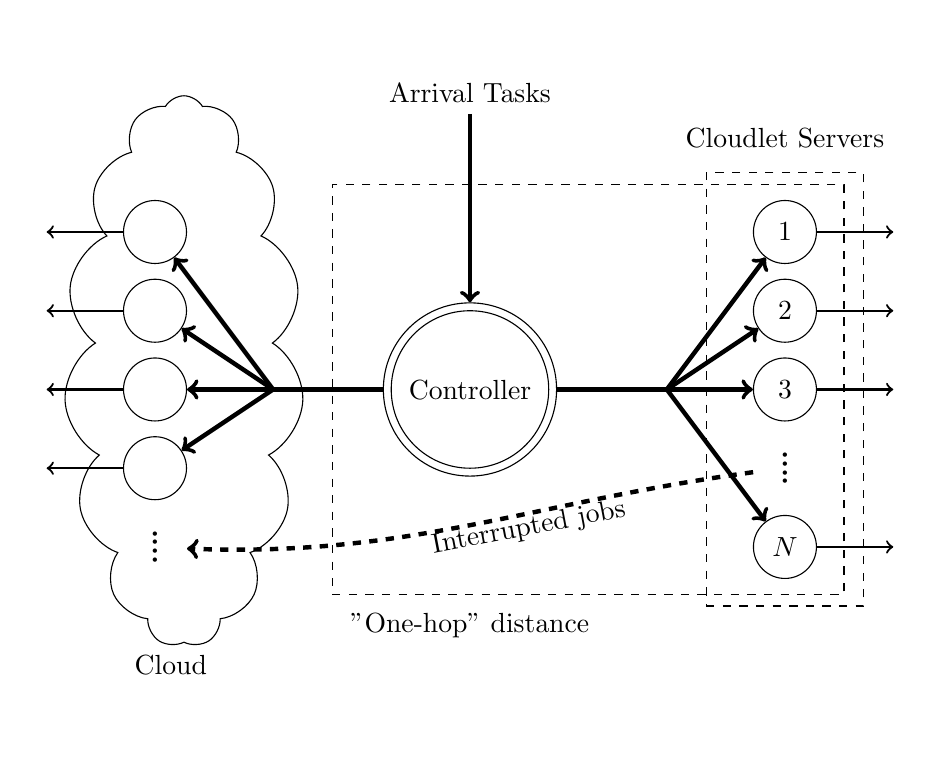
\begin{tikzpicture}


% Cloud

\node[circle, draw, minimum width = 0.8cm]        					   (CloudNode0) at (0,2) {};
\node[circle, draw, minimum width = 0.8cm, below of=CloudNode0]        (CloudNode1) {};
\node[circle, draw, minimum width = 0.8cm, below of=CloudNode1]        (CloudNode2) {};
\node[circle, draw, minimum width = 0.8cm, below of=CloudNode2]        (CloudNode3) {};
\node[circle, draw=white, minimum width = 0.8cm, below of=CloudNode3]  (CloudNode4) {\rotatebox{90}{\textbf{....}}};

\node[above of=CloudNode4, yshift=-2.5cm, xshift=0.2cm] (labellllllll) {Cloud};

\node[right of=CloudNode0, xshift=-2.5cm] (ExtCloudNode0) {};
\node[right of=CloudNode1, xshift=-2.5cm] (ExtCloudNode1) {};
\node[right of=CloudNode2, xshift=-2.5cm] (ExtCloudNode2) {};
\node[right of=CloudNode3, xshift=-2.5cm] (ExtCloudNode3) {};


\coordinate (cloudStartNode) at (1.5,0);

% Controller

\node[circle, draw, minimum width = 2.2cm]  (ControllerExternal) at (4,0) {};
\node[circle, draw, minimum width = 2cm]    (Controller2)        at (4,0) {Controller};

\coordinate (cloudletStartNode) at (6.5,0);

\coordinate (Start) at (4,3.5);

% Cloudlet

\node[circle, draw, minimum width = 0.8cm, left of=ControllerExternal, xshift=5cm, yshift=2cm]       (CloudletNode0) {$1$};
\node[circle, draw, minimum width = 0.8cm, below of=CloudletNode0]           (CloudletNode1) {$2$};
\node[circle, draw, minimum width = 0.8cm, below of=CloudletNode1]           (CloudletNode2) {$3$};
\node[circle, draw=white, minimum width = 0.8cm, below of=CloudletNode2]     (CloudletNode3) {\rotatebox{90}{\textbf{....}}};
\node[circle, draw, minimum width = 0.8cm, below of=CloudletNode3] (CloudletNode4) {$N$};

\node[rectangle, draw, dashed, minimum width =6.5cm, minimum height=5.2cm] (Cloudlet) at (5.5,0) {};
\node[circle,below of=Cloudlet, yshift=-2cm, xshift=-1.5cm] (label1) {"One-hop" distance};

\node[left of=CloudletNode0, xshift=2.5cm] (ExtCloudletNode0) {};
\node[left of=CloudletNode1, xshift=2.5cm] (ExtCloudletNode1) {};
\node[left of=CloudletNode2, xshift=2.5cm] (ExtCloudletNode2) {};
\node[left of=CloudletNode4, xshift=2.5cm] (ExtCloudletNode3) {};

\node[rectangle, draw, dashed, minimum width =2cm, minimum height=5.5cm, right of=CloudletNode2, xshift=-1cm] (CloudletFrame) {};
\node[circle,above of=CloudletFrame, yshift=2.2cm] (label1) {Cloudlet Servers};

% Cloudlet Rows...

\draw[ultra thick,-] (ControllerExternal) -- (cloudletStartNode);
\draw[ultra thick,->] (cloudletStartNode) -- (CloudletNode0);
\draw[ultra thick,->] (cloudletStartNode) -- (CloudletNode1);
\draw[ultra thick,->] (cloudletStartNode) -- (CloudletNode2);
\draw[ultra thick,->] (cloudletStartNode) -- (CloudletNode4);

% Cloud Rows...

\draw[ultra thick,-] (ControllerExternal) -- (cloudStartNode);
\draw[ultra thick,->] (cloudStartNode) -- (CloudNode0);
\draw[ultra thick,->] (cloudStartNode) -- (CloudNode1);
\draw[ultra thick,->] (cloudStartNode) -- (CloudNode2);
\draw[ultra thick,->] (cloudStartNode) -- (CloudNode3);

% Out from cloudlet nodes

\draw[thick,->] (CloudletNode0) -- (ExtCloudletNode0);
\draw[thick,->] (CloudletNode1) -- (ExtCloudletNode1);
\draw[thick,->] (CloudletNode2) -- (ExtCloudletNode2);
\draw[thick,->] (CloudletNode4) -- (ExtCloudletNode3);

% Out from cloud nodes

\draw[thick,->] (CloudNode0) -- (ExtCloudNode0);
\draw[thick,->] (CloudNode1) -- (ExtCloudNode1);
\draw[thick,->] (CloudNode2) -- (ExtCloudNode2);
\draw[thick,->] (CloudNode3) -- (ExtCloudNode3);
 
% START

\draw[ultra thick,->] (Start) node[above] {Arrival Tasks} -- (ControllerExternal) ;

\node [cloud, right of=CloudNode3, xshift=-18, yshift=35, draw,cloud puffs=15,cloud puff arc=120, aspect=3, minimum width =2.5cm, minimum height=7cm, inner ysep=1em] (cloudcc) {};

\path (CloudletNode3) edge[->,dashed,ultra thick, bend left, out=0, in=170] node [left] [sloped, yshift=-5,xshift=60] {Interrupted jobs} (CloudNode4);

\end{tikzpicture}
\caption{System diagram.} \label{figure:SystemDiagram}
\end{figure}



As known, building a system \textit{conceptual model} means to describe it highlighting which state variables are important specifying how they are interrelated.\footnote{\textit{Ibid.}}

Our system represents a network of nodes to which some application, running in a set of external mobile devices, send their tasks, called \textit{jobs} or \textit{task}, because of performance or energy saving reasons. Not all jobs sent to system are the same, in fact we distinguish two class type of jobs, that is \textit{class 1} and \textit{class 2} type jobs.

To minimize mean response time experienced by mobile device users, the system is been built as a \textit{two-layer} network in such a way that any arriving job is sent, if possible, to the nearest node to be run.

To be more precise, as you can see from figure \ref{figure:SystemDiagram}, our system is made up of a set of nodes including:

\begin{description}
\item[Cloudlet node] Also called \textit{edge cloud server}, it is a computer cluster located at an "\textit{one-hop}" distance from mobile devices users, that is very close to them, therefore network delay experienced is very low. That cluster is able to guarantee absence of interferences among tasks allocated to it as long as their number does not exceed a given threshold $N$. 

Consequently, from our conceptual model point of view, cloudlet node represents a \textit{fixed-capacity multi-server service node with no queue} which capacity, that is the maximum possible number of jobs in it, is fixed to $N$. 

Since jobs inter-arrival times and service times are \textit{exponentially} distributed according to our project specification, a queuing model able to properly represent that node is the M/M/N/N queueing model system\footnote{Mor Harchol-Balter, \textit{Performance Modeling and Design of Computer Systems} (Carnegie Mellon University, Pennsylvania 2013), 255-256} although there is a very important different with it: due to adopted routing policies, when cloudlet node is "\textit{full}" and so not capable to run a further job, any arriving job is forwarded somewhere else rather than to cloudlet node, therefore no jobs are really lost.

\item[Cloud node] Also called \textit{remote cloud server}, it is another computer cluster which, although it \textit{suffers for greater network delay}, due of its high distance from mobile devices, being virtually made up of unlimited number of servers, has \textit{unlimited resources}, therefore it can to process any number of tasks allocated to it. 

Consequently we had modelled this system's node as an \textit{unlimited-capacity multi-server service node with no queue}. 

Since, as we previously said, jobs inter-arrival and service times are exponential, due to the presence of an infinite number of server, such a system's node can be modelled by  a M/M/$\infty$ queueing model system.\footnote{\textit{Ibid.}, 271}. 


\item[Controller node] It represents system's entry point being all arriving jobs sent firstly to it by mobile devices. Its duty is to decide about whether an arrived job should be sent to cloudlet or cloud node according to adopted routing policy.

It is located at the same distance of cloudlet node from mobile devices users, therefore, also in this case, network delay experienced is very low. Although it can run only one job at a time, it has the capability to process each arriving job \textit{instantaneously}. 

We have simply modelled it as \textit{single-server service node with no queue}. It's correspondent queuing model system is M/M/1.

\end{description}




\begin{algorithm}

\caption{}\label{alg:accessControlAlgorithm1}

\begin{algorithmic}[1]

\Function{accessControlFunction}{$\textit{arrivalJob}$}

\If {$(n_1 + n_2=N)$}
	\State Send $\textit{arrivalJob}$ on the cloud.
\Else 	
 	\State Send $\textit{arrivalJob}$ on the cloudlet.
\EndIf

\EndFunction

\end{algorithmic}
\end{algorithm}

At this point, in order to properly define our conceptual model, we need to specify which \textit{system state variables} are truly important for our goals.

A complete characterization of the our system state is simply provided by the number of each class jobs running both on cloudlet and cloud node at a given instant of time; we will formalize this statement in the next section where we will provide relations and computation methods too. 

For now we have to just focus on routing policies. As we previously said, there are two type of access control algorithms used by controller node to make decisions; they are fully described by pseudo-code shown in Algorithm \ref{alg:accessControlAlgorithm1} and Algorithm \ref{alg:accessControlAlgorithm2}. Note that you can use only one access control algorithm type a during a simulation run.

Although they are both \textit{work-conserving scheduling policy}, that is they always perform work on some job when there is a job in the system,\footnote{\textit{Ibid.}, Definition 28.1, page 474} there is one difference between them: access control algorithms 1 does not provide job pre-emption once it starts service on cloudlet node unlike access control algorithms 2, which provides, instead, pre-emption when some condition are achieved requiring also a set-up time to restart interrupted job (note that Algorithm \ref{alg:accessControlAlgorithm2} use a further threshold variable to make its decision denoted by $S$ which is less or equal than $N$).


\begin{algorithm}[h]
\caption{}\label{alg:accessControlAlgorithm2}
\begin{algorithmic}[h!]

\Function{accessControlFunction}{$\textit{arrivalJob}$}

\If {$(\textit{arrivalJob.isClassOne})$}


\If {$n_1 = N$}
	\State Send $\textit{arrivalJob}$ on the cloud.

\ElsIf{$n_1 + n_2 \leq S $}
	\State Send $\textit{arrivalJob}$ on the cloudlet.
\ElsIf{$ n_2 \geq 0 $}
	\State Interrupt a class 2 job currently running on cloudlet.
	\State Send interrupted job to cloud.
	\State Send $\textit{arrivalJob}$ on the cloudlet.
\Else 	
 	\State Send $\textit{arrivalJob}$ on the cloudlet.
\EndIf



\Else 

\If {$(n_1 + n_2 \geq S)$}
	\State Send $\textit{arrivalJob}$ on the cloud.
\Else 	
 	\State Send $\textit{arrivalJob}$ on the cloudlet.
\EndIf

\EndIf

\EndFunction

\end{algorithmic}
\end{algorithm}
















\clearpage
\newpage
\section{Specification  Model}

In this section we will provide a \textit{specification model} of our system in which we will turn all system's states into a collection of mathematical variables together with equations and logic describing how the state variables are interrelated including algorithms for computing their interaction and evolution in time.\footnote{Lawrence M. Leemis, Stephen K. Park, \textit{Discrete-Event Simulation: A First Course} (Pearson; 1 edition January 6, 2006), 186}

In other words, we will provide:

\begin{itemize}
\item A set of mathematical state variables that together provide a complete system description.
\item A set of system event types.
\item A collection of mathematical methods that will take place when each type of event occurs in order to update system state variables.
\end{itemize}

\subsection{System's variables}

In order to properly describe all system's state variables, we need to introduce some mathematical notations.

$\tau \in (t_0, t)$ denotes a time's instant of our system simulation clock where $t_0$ and $t$ represent respectively \textit{start moment} and \textit{final moment} of our simulation; we will use also $c \in \lbrace 1,2 \rbrace = C$, representing the class to which a job belongs, and $x \in \lbrace cloudlet,cloud,global \rbrace = X$, used, instead, to refer to a specific system's node or to the whole system.

At this point we can introduce all mathematical variables used in our model:

\begin{table}[h!]
    \centering
    \small
    \begin{tabular}{rcl}
       
      $n_x^{(c)}(\tau)$ & $ = $ & Number of class $c$ jobs currently running at $x$ system's node at time $\tau$ \\
      $d_x^{(c)}(\tau)$ & $ = $ & Number of class $c$ departed jobs from node $x$ at time $\tau$ \\
      $s_{x,i}^{(c)}$ & $ = $ & Service time of class $c$ job $i$ served on $x$ node   \\
      $i_{cloudlet}^{(2)}(\tau)$ & $ = $ & Number of class 2 interrupted jobs at time $\tau$ which were running on cloudlet\\
          
    \end{tabular}
\end{table}

We define the \textit{state} of our system at time $\tau$ as follows:

\begin{equation}
\omega(\tau) = (\omega_{cloudlet}(\tau),\omega_{cloud}(\tau))
\end{equation}

Where $\omega_{cloudlet}(\tau)$ and $\omega_{cloud}(\tau)$ are, respectively, cloudlet and cloud node state at time $\tau$. Specifically:

\begin{equation}
\begin{array} {rcl} 
\omega_{cloudlet}(\tau) & = & (n_{cloudlet}^{(1)}(\tau),n_{cloudlet}^{(2)}(\tau)) \\
\omega_{cloud}(\tau) & = & (n_{cloud}^{(1)}(\tau),n_{cloud}^{(2)}(\tau)) \\
\end{array}
\end{equation}

Thus:

\begin{equation}
\begin{array} {rcl} 
\omega(\tau) = ((n_{cloudlet}^{(1)}(\tau),n_{cloudlet}^{(2)}(\tau)),(n_{cloud}^{(1)}(\tau),n_{cloud}^{(2)}(\tau))
\end{array}
\end{equation}

At this point we can show some equations describing constrains or relations among these variables.

Obliviously is true that:

\begin{equation}
\begin{array} {lr} 
\displaystyle n_{global}^{(c)}(\tau) = \sum_{x \in X \setminus \lbrace global \rbrace } n_x^{(c)}(\tau) & \forall c \in C, \forall \tau \in (t_0, t)
\end{array}
\end{equation}

\begin{equation}
\begin{array} {lr} 
\displaystyle d_{global}^{(c)}(\tau) = \sum_{x \in X \setminus \lbrace global \rbrace } d_x^{(c)}(\tau) & \forall c \in C, \forall \tau \in (t_0, t)
\end{array}
\end{equation}

If our system is based on Algorithm \ref{alg:accessControlAlgorithm1}, is true that:

\begin{equation}
\begin{array} {lr} 
\displaystyle \sum_{c \in C} n_{cloudlet}^{(c)}(\tau) \leq N & \forall \tau \in (t_0, t)
\end{array}
\end{equation}

When, instead, our system is using Algorithm \ref{alg:accessControlAlgorithm2}, is verified that:

\begin{equation}
\begin{array} {rccr} 
\displaystyle \sum_{c \in C} n_{cloudlet}^{(c)}(\tau) \leq S & \Leftrightarrow & n_{cloudlet}^{(2)}(\tau) > 0 & \forall \tau \in (t_0, t) \\
n_{cloudlet}^{(1)}(\tau) \leq N & \Leftrightarrow & n_{cloudlet}^{(2)}(\tau) = 0 & \forall \tau \in (t_0, t)
\end{array}
\end{equation}

\subsection{Statistics computing}

During this subsection we will describe how we can compute all system's statistics which we need using mathematical notation explained before.

\paragraph{Time-averaged population}

In order to compute $E[N_x]^{(c)}$, that is the \textit{time-averaged number of $c$ class jobs in $x$ system's node}, we can do as follows:\footnote{\textit{Ibid.}, 19}

\begin{equation}
\begin{array} {rclr} 
E[N_x]^{(c)} & = & \displaystyle  \dfrac{1}{t-t_0}\int_{t_0}^t n_x^{(c)}(\tau)d\tau & \forall c \in C, \forall x \in X
\end{array}
\end{equation}

To calculate instead $E[N_x]$, \textit{not-class-based time-averaged number of jobs running in a $x$ system's node}, we can proceed as shown below:

\begin{equation}
\begin{array} {rclr} 
E[N_x] & = & \displaystyle  \dfrac{1}{t-t_0} \cdot \int_{t_0}^t \left( n_x^{(1)}(\tau) + n_x^{(2)}(\tau) \right) d\tau \\\\
	   & = & \displaystyle  \dfrac{1}{t-t_0} \cdot \int_{t_0}^t n_x^{(1)}(\tau)d\tau + \dfrac{1}{t-t_0} \cdot \int_{t_0}^t n_x^{(2)}(\tau)d\tau \\\\
	   & = & E[N_x]^{(1)} + E[N_x]^{(2)} \\\\
	   & = & \displaystyle  \sum_{c \in C} E[N_x]^{(c)} & \forall x \in X
\end{array}
\end{equation}

\paragraph{Time-average response time}

Are $E[S_x]^{(c)}$ and $E[T_x]^{(c)}$, respectively, the \textit{time-averaged service time and response time of class $c$ jobs in $x$ system's node}. 

Since our system hasn't queues, there is no waiting time or delay experienced by jobs in our system, therefore result that $E[S_x]^{(c)} = E[T_x]^{(c)}$.
Said that, we just have to show how to compute $E[S_x]^{(c)}$:\footnote{\textit{Ibid.}, 17}

\begin{equation}
\begin{array} {rccccr} 
E[T_x]^{(c)} & = & E[S_x]^{(c)} & = & \displaystyle \dfrac{1}{d_x^{(c)}(t)} \cdot \sum_{i = 0}^{d_x^{(c)}(t)} s_{x,i}^{(c)} & \forall c \in C, \forall x \in X \\
\end{array}
\end{equation}

If we aren't interested about per-class metrics, we can compute $E[S_x]$ and $E[T_x]$, respectively \textit{time-averaged service time} and the \textit{time-averaged response time experienced by any class jobs in a $x$ system's node}, we can do as follows:

\begin{equation}
\begin{array} {rccccr} 
E[T_x] & = & E[S_x] & = & \displaystyle \dfrac{1}{d_x^{(1)}(t) + d_x^{(2)}(t)} \cdot \left( \sum_{i = 0}^{d_x^{(1)}(t)} s_{x,i}^{(1)} + \sum_{i = 0}^{d_x^{(2)}(t)} s_{x,i}^{(2)} \right) & \forall x \in X \\
\end{array}
\end{equation}

\paragraph{Throughput}

\textit{Per-class system's node throughput}, denoted with $X_x(c)$, is the rate of per-class $c$ completions at $x$ system's node, while \textit{system's node throughput}, indicated with $X_x$, is the rate of any class job completions at $x$ system's node\footnote{Mor Harchol-Balter, \textit{Performance Modeling and Design of Computer Systems} (Carnegie Mellon University, Pennsylvania 2013), 18}. 

Generally the throughput is the ratio between the total number of jobs completed and observation time\footnote{\textit{Ibid.}}, therefore aforesaid metrics are simply computable as follows:

\begin{equation}
\begin{array} {rccr} 
X_x(c) & = & \displaystyle \dfrac{d_x^{(c)}(t)}{t} & \forall c \in C, \forall x \in X \\
\end{array}
\end{equation}

\begin{equation}
\begin{array} {rccr} 
X_x & = & \displaystyle \dfrac{d_x^{(1)} + d_x^{(2)}(t)}{t} & \forall x \in X \\
\end{array}
\end{equation}

\paragraph{Percentage class 2 job interruptions}

Is $p^{(2)}_{interruption}$ the percentage class 2 job interruptions previously running on cloudlet. Note that this metric is computable only when our simulation is using access control algorithm 2.

To compute them we can simply do:

\begin{equation}
\begin{array} {rccr} 
p^{(2)}_{interruption} & = & \displaystyle \dfrac{i_{cloudlet}^{(2)}(t)}{d_{global}^{(2)}(t)} \\ 
\end{array}
\end{equation}

\subsection{System's assumptions}

To complete to turn out our conceptual model into a proper specification model, we have to make additional assumptions which we have reported below:

\begin{itemize}
\item Although initial state variables can have any non-negative integer value\footnote{\textit{Ibid.} 190}, we have choosen, as common, to set $n_x^{(c)}(0) = 0$ and $d_x^{(c)}(0) = 0$ setting, in this way, initial system status as \textit{idle}. 

\item As a consequence of the previous point, first event must be either a class 1 or class 2 job arrival on controller node.

\item Terminal state is also idle. Rather than specifying the number of jobs processed, our stopping criteria has been specified in terms of a time $\tau^*$ beyond which no new jobs can arrive. This assumption effectively closes the door at time $\tau^*$ but allows the system to continue operation until all jobs have been completely served. 

Therefore, the last event must be either a class 1 or class 2 job completion.
\end{itemize}


\subsection{System's events and assumptions}

Let's look to all possible \textit{events} which can occurs during our simulations. 

Since by definition any event is an occurrence that may change the state of the system\footnote{Lawrence M. Leemis, Stephen K. Park, \textit{Discrete-Event Simulation: A First Course} (Pearson; 1 edition January 6, 2006), 187}, obviously our system's state variables can change only when an event occurs.

All event capable to alter our system's state and their effect on state variables are reported in table \ref{table:SystemEvents} but pay attention to the fact that all events reported just focus on access control algorithm 1 based system. When you use access control algorithm 2, you have to remember that, when a class 1 job arrival on cloudlet node occurs, a class 2 job may be interrupted if algorithm \ref{alg:accessControlAlgorithm2} conditions would be achieved; in this case $n_{\text{cloudlet}}^{(1)}(\tau)$ are then incremented by one while $n_{\text{cloudlet}}^{(2)}(\tau)$ is decremented by one and a class 2 job arrival is scheduled.
 
\begin{table}[h!]
    \caption{Access control algorithm 1 system's events}
    \begin{adjustbox}{center=\textwidth}
    \label{table:SystemEvents}
     \begin{tabular}{c|c|p{2.5cm}}

      \toprule
      \textbf{Event name that occurred at time $\tau$} & \textbf{Event's place} & \textbf{Event's effects} \\
      \midrule
      
      \multirow{3}{*}{Class 1 job arrival} & Cloudlet & $n_{\text{cloudlet}}^{(1)}(\tau)\texttt{++}$ \\ \cline{2-3} 
      & Cloud & $n_{\text{cloud}}^{(1)}(\tau)\texttt{++}$ \\ \cline{2-3} 
      & Controller & $n_{\text{global}}^{(1)}(\tau)\texttt{++}$ \\ 
       
      \hline
       
      \multirow{3}{*}{Class 2 job arrival} & Cloudlet & $n_{\text{cloudlet}}^{(2)}(\tau)\texttt{++}$ \\ \cline{2-3} 
      & Cloud & $n_{\text{cloud}}^{(2)}(\tau)\texttt{++}$ \\ \cline{2-3} 
      & Controller & $n_{\text{global}}^{(2)}(\tau)\texttt{++}$ \\ 
    
	  \hline
       
      \multirow{8}{*}{Class 1 job departure} & \multirow{4}{*}{Cloudlet} & $n_{\text{cloudlet}}^{(1)}(\tau)\texttt{--}$ \newline $n_{\text{global}}^{(1)}(\tau)\texttt{--}$ \newline $d_{\text{cloudlet}}^{(1)}(\tau)\texttt{++}$ \newline $d_{\text{global}}^{(1)}(\tau)\texttt{++}$ \\ \cline{2-3} 
      & \multirow{4}{*}{Cloud} & $n_{\text{cloud}}^{(1)}(\tau)\texttt{--}$ \newline $n_{\text{global}}^{(1)}(\tau)\texttt{--}$ \newline $d_{\text{cloud}}^{(1)}(\tau)\texttt{++}$ \newline $d_{\text{global}}^{(1)}(\tau)\texttt{++}$ \\ \cline{2-3} 
 
 		\hline
       
      \multirow{8}{*}{Class 2 job departure} & \multirow{4}{*}{Cloudlet} & $n_{\text{cloudlet}}^{(2)}(\tau)\texttt{--}$ \newline $n_{\text{global}}^{(2)}(\tau)\texttt{--}$ \newline $d_{\text{cloudlet}}^{(2)}(\tau)\texttt{++}$ \newline $d_{\text{global}}^{(2)}(\tau)\texttt{++}$ \\ \cline{2-3} 
      & \multirow{4}{*}{Cloud} & $n_{\text{cloud}}^{(2)}(\tau)\texttt{--}$ \newline $n_{\text{global}}^{(2)}(\tau)\texttt{--}$ \newline $d_{\text{cloud}}^{(2)}(\tau)\texttt{++}$ \newline $d_{\text{global}}^{(2)}(\tau)\texttt{++}$ \\
 
      \bottomrule


    \end{tabular}
    \end{adjustbox}
\end{table}




\clearpage
\newpage
\section{Computational Model}

Let's start now the description of our system \textit{computational model} in which, as known, system's states exist as a collection of data structure, classes and variables that collectively characterize the system and are systematically updated as simulated time evolves.

Our model is been implemented using Java programming languages, which source code is fully available on GitHub\footnote{Source code available on \texttt{https://github.com/AndreaG93/PMCSN-Project}}, famous web-based hosting service for version control using \texttt{git}; we remind that \LaTeX\ source code of this report is available too.\footnote{See \texttt{https://github.com/AndreaG93/PMCSN-Project-Report}}

\begin{figure}[H]
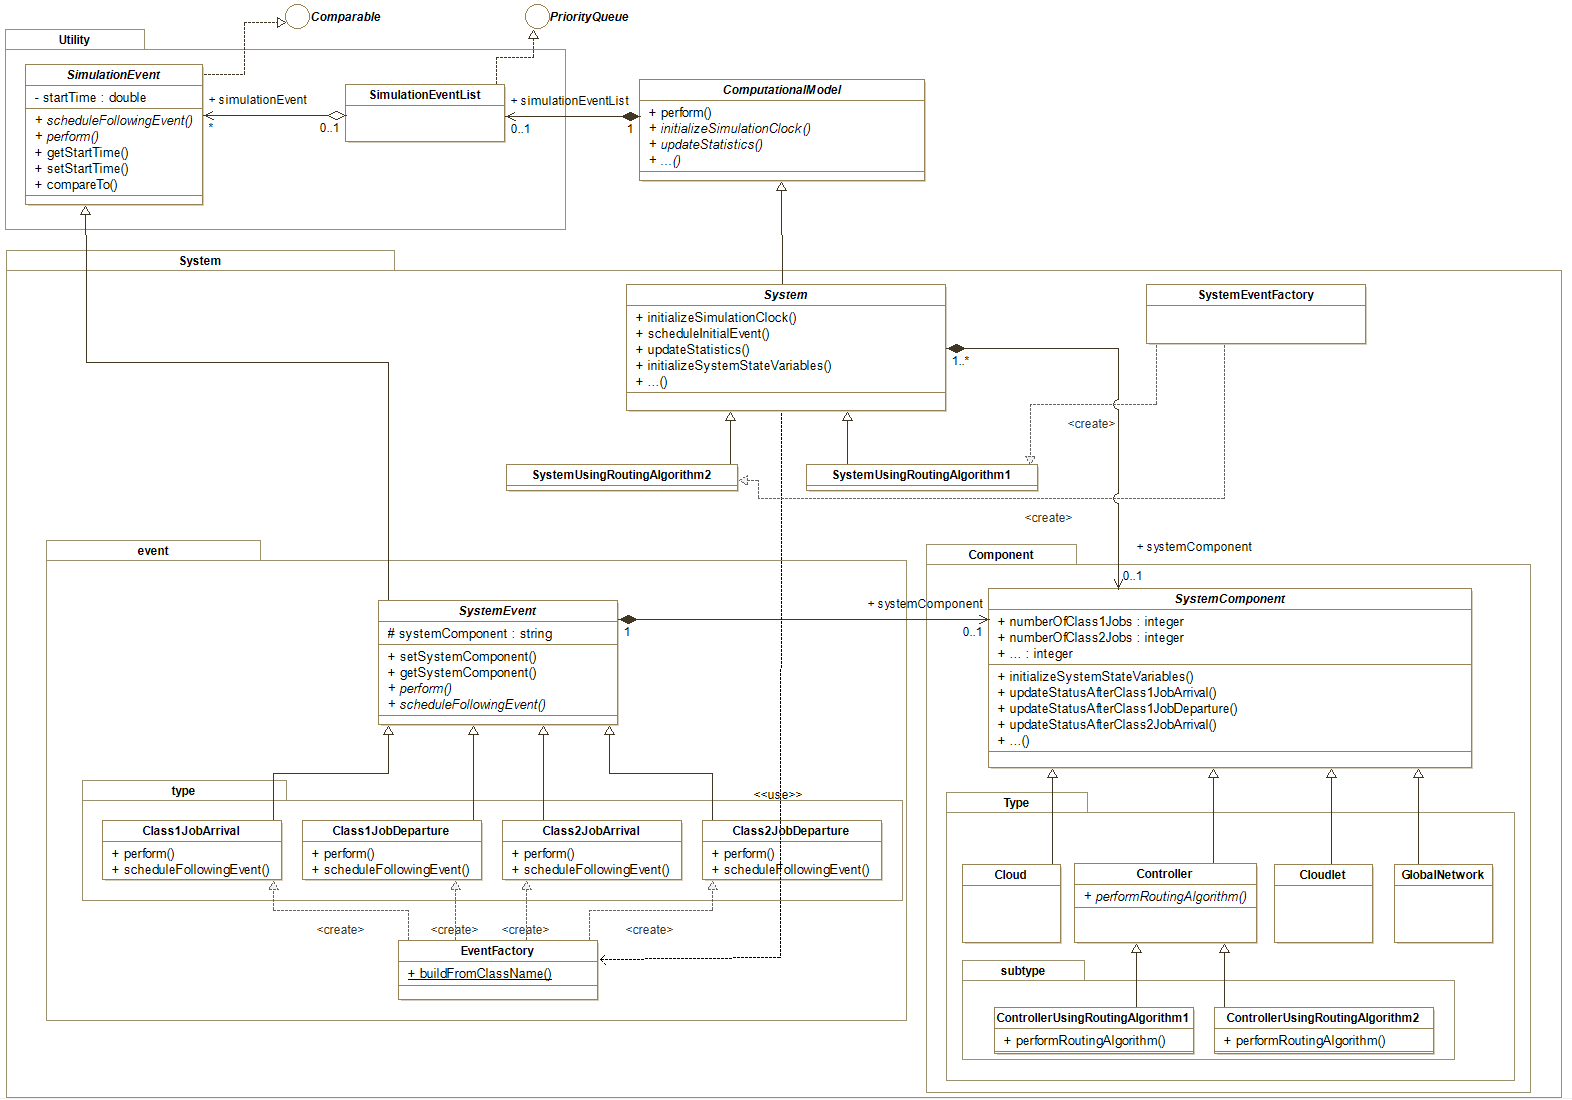
\includegraphics[width=\textwidth]{ClassDiagram}
\centering
\caption{Class diagram showing main classes and methods only.}

\label{fig:ClassDiagram}

\end{figure}


\subsection{Events implementation}

In order to properly describe how our implementation works we need to understand how all system's events, seen in previous section, are represented and managed.

As you can see in the class diagram \ref{fig:ClassDiagram}, a \textit{generic} system's event has been implemented and represented using an \textit{abstract} Java class called \texttt{SimulationEvent} (located into \texttt{nexteventsimulation.\-utility} Java package) which has two main features:

\begin{itemize}
\item Has only one \texttt{double} type field, called \texttt{StartTime}, which is used to hold the instant of time according to which an event occurs. Setter and getter methods are provided in order to manage this field.

\item It declares two very important abstract methods which, as we will can see later, are called by next-event simulation algorithm implemented in \texttt{ComputationalModel} class; these methods are called \texttt{perform()}, whose purpose is to update system's state variables when an event occurs, and \texttt{schedule\-Following\-Event()}, which is used, instead, to inserts into an \textit{event list} events that follows the current one.

Although is obvious that exact methods behaviour depends strictly by which concrete class implements them, is however very important to point out that \texttt{SimulationEvent} class does \textit{not} represent system-specific events. In fact, to ensure low coupling and high cohesion among classes, neither \texttt{SimulationEvent} or \texttt{ComputationalModel} class need to know any specific system information. 
\end{itemize}

System-specific event are instead represented by instances of \texttt{SystemEvent} class (located into \texttt{nexteventsimulation.computationalmodel.model.\-sy\-stem.\-ev\-ent} package) whose code is partially shown in Listing \ref{code:SystemEvent}. 


\begin{lstlisting}[frame=lines, caption={\texttt{SystemEvent} class implementation.}, label={code:SystemEvent}]
public abstract class SystemEvent extends SimulationEvent {

    protected SystemComponent systemComponent;

    public void setSystemComponent(SystemComponent systemComponent) {
        this.systemComponent = systemComponent;
    }

    public SystemComponent getSystemComponent() {
        return systemComponent;
    }
    ...
\end{lstlisting}

As you can see from reported snipped, \texttt{SystemEvent} class has a \texttt{SystemCom\-po\-nent} type field, called \texttt{systemComponent}, which is used to hold a reference to that system's node where a generic event occurs; in this way any \texttt{SystemEvent} instance is able to update state variables of the component of which it has the reference, without altering others parts of system.

However, in order to do that, required abstract method implementation is needed. In our implementation there are four concrete \texttt{SystemEvent} type classes used to represents all system's events:

\begin{itemize}
\item \texttt{Class1JobArrival} class which represents a class 1 job arrival.
\item \texttt{Class2JobArrival} class which models a class 2 job arrival.
\item \texttt{Class1JobDeparture} class is used to model a class 1 job departure.
\item \texttt{Class2JobDeparture} class for class 2 jobs departures.
\item \texttt{PreviouslyInterruptedClass2JobArrival} this class (not displayed in class diagram shown in Figure \ref{fig:ClassDiagram}) represents a class 2 jobs arrival which is been previously interrupted on cloudlet node.
\item \texttt{PreviouslyInterruptedClass2JobDeparture} like previous one but focused on class 2 jobs departure.
\end{itemize}

Any instance of above classes, having knowledge about methods published by \texttt{SystemComponent} class, can update states of any component of our system. In this way we can achieve an high degree of cohesion among classes and low coupling taking advantage of polymorphism pattern; in fact, as we can see also from shown class diagram, \texttt{ComputationalModel} class has to know only about \texttt{SimulationEvent} class and, thorough invocation of its methods, being able to update our system ignoring all specific information about our system.

\subsection{Event list}

As known, an \textit{event list}, also called \textit{calendar}, represents a data structure used to keep track of scheduled time of occurrence for the next possible event.

For reasons of efficiency, our event list is been implemented as a \textit{min-heap binary tree}, that is a \textit{priority queue} in which all events are ordered by time, in such a way that the most imminent event is found on the tree's root. This data structure is able to provide $O(log_2(n))$ time for the en-queuing and dequeuing operations and constant time for root element retrieval.\footnote{Camil Demetrescu, Irene Finocchi, Giuseppe F. Italiano - \textit{Algorimti e strutture dati} - second edition, McGraw-Hill, pag. 200} 

Fortunately a Java implementation is already available in JDK through built-in class called \texttt{PriorityQueue$<$E$>$} which provides all method that we need, like \texttt{poll}, for root element retrieval, \texttt{add} and \texttt{remove}, used respectively for en-queuing and dequeuing operations.

However, in order to that data structure works properly, is required that a total ordering among all possible event exists. To provide it, we need that all \texttt{SimulationEvent} type instances implement an interface called \texttt{Comparable} providing an implementation, shown in listing \ref{code:compareTo}, of a method called \texttt{compareTo}.\footnote{See \texttt{https://docs.oracle.com/en/java/javase/12/docs/api/java.base/java/lang/Comparable.html\#compareTo(T)}} In this way, is very easy to order all \texttt{SimulationEvent} type instances based on their start event time, from the youngest to the oldest. 

\begin{lstlisting}[frame=lines, caption={Snippet of \texttt{SimulationEvent} class implementation}, label={code:compareTo}]
@Override
public int compareTo(SimulationEvent o) {
	return Double.compare(this.startTime, o.startTime);
}
\end{lstlisting}

\subsection{Simulation clock}

As we know a \textit{simulation clock} is necessary to keep track of the current value of simulated time during simulation. 

In our system's implementation, our simulation clock is represented by a \texttt{SimulationClock} type instance, whose code is partially reported in Listing \ref{code:SimulationClock}. 

Simulation clock state is represented by two \texttt{double} type fields: the first, called \texttt{currentEventTime}, is used to holding current simulated time value, while the second, called \texttt{nextEventTime}, is used instead to keep track of next event simulated time value; obviously, proper setter and getter methods are provided in order to manage them.

From software architecture point of view, believing that multiple \texttt{Simulation\-Clock} instance are not necessary for our purposes, we have choosen to design this class using the \textit{singleton} pattern. 

\begin{lstlisting}[frame=lines, caption={\texttt{SimulationClock} class implementation.}, label={code:SimulationClock}]
public class SimulationClock {

    private static SimulationClock instance = null;

    private double currentEventTime;
    private double nextEventTime;

    private SimulationClock(){
    }

    public static SimulationClock getInstance() {
        if (instance == null)
            instance = new SimulationClock();
        return instance;
    } 
    ...
\end{lstlisting}


\subsection{Next-event simulation logic}

The most important code is included into \texttt{ComputationalModel} class because it contains main simulation logic.

To start a next-event simulation is very easy because we just need to invoke an its method called \texttt{perform} which contains the algorithm\footnote{Lawrence M. Leemis, Stephen K. Park, \textit{Discrete-Event Simulation: A First Course} (Pearson; 1 edition January 6, 2006), Algorithm 5.1.1, page 189} used to perform a simulation based on next-event approach, whose Java implementation is reported in Listing \ref{code:perform}. Our algorithm consists of the following steps: 

\begin{description}
\item[Simulation initialization] As phase name suggests, during this step system state variables, simulation clock, event list and everything is needed for simulation is initialized compatibly with what we have described in previous section, during specification model analysis.

Remember that \texttt{ComputationalModel} is an abstract class which knows anything about our specific system, therefore, obviously, system initialization phase differs according to which concrete class implements that class. Anyhow, as you can see from code snippet reported below, this task is performed invoking \texttt{initialize\-Simulation()} method; that invocation represents a short-cut used to call a large set of abstract methods for initialization purposes, like \texttt{initializeSystemStateVariables}, \texttt{initializeSimulationClock} and \texttt{scheduleInitialEvent}.

\item[Process current event] Although we believe the code is self explanatory, we sum up this phase as follows: until event list is not empty (line 6), the most imminent possible event is extracted and removed from event list (line 8); then simulation clock is advanced to this event's scheduled time of occurrence (line 12) and finally system state is updated (line 14). 

\item[Schedule following event] Until a fixed simulation time $\tau^*$ in not exceeded, a new event is generated by current event and consequently placed into event list. Subsequently simulation clock state is updated in order to compute some system metrics.

\item[Statistic update] While simulation advance from one event time to the next, through an invocation to an abstract method called \texttt{updateStati\-stics}, is possible to update some variables for system's statistic metrics computation.

\item[Simulation result generation] During this final step, all collected data are elaborated using various approaches, producing some statistic metrics including graphics like histograms or scatter plots. We will examine involved classes later.
\end{description}

\begin{lstlisting}[frame=lines, caption={Snippet of \texttt{perform} method}, label={code:perform}]
public void perform() {

        initializeSimulation();

        while (!this.simulationEventList.isEmpty()) {

            SimulationEvent actualEvent = this.simulationEventList.poll();

            if (actualEvent != null) {

                SimulationClock.getInstance().setCurrentEventTime(actualEvent.getStartTime());

                actualEvent.perform();
                actualEvent.scheduleFollowingEvent();

                SimulationEvent nextEvent = this.simulationEventList.peek();

                if (nextEvent != null)
                    SimulationClock.getInstance().setNextEventTime(nextEvent.getStartTime());
            }
            updateStatistics();
        }

        BatchMeansRegister.getInstance().computeStatisticsAndWriteData();
        ScatterPlotRegister.getInstance().writingOutputData();
        HistogramsRegister.getInstance().computeStatisticsAndWriteData();

        manageCurrentSimulationResult();
    }
\end{lstlisting}


\subsection{System network implementation}

As we have seen in previous subsection, \texttt{ComputationalModel} is used to represent a very \textit{generic} form of system (or queues network) because it includes only the code, seen previously, used to perform a next-event simulation.  

In fact, we have used another abstract class to represent our specific queues network; that class, which also provide the implementation of all previously mentioned required methods in order to perform our simulation, is called \texttt{System}.

Although a \texttt{System} type instance represents our specific queues network, it however do \textit{not} contain any system state variables and do \textit{not} perform any statistic metric computation about them; its main purpose is to hold a reference to any system's node, represented by \texttt{SystemComponent} objects, in order to manage them. 

In fact the state of a \texttt{System} type instance is made up of four \texttt{SystemComponent} type fields which are used to hold a reference to all system's components: cloud, cloudlet and controller. An extra \texttt{SystemComponent} type field is used as a convenient short-cut to represent the global system.

Its other responsibilities are:

\begin{itemize}

\item Allocation and management of all \texttt{SystemComponent} type objects.

\item Methods implementation providing for simulation clock and system nodes state variables initialization.

\item Event scheduling management through some methods invocations like \texttt{sche\-dule\-Event\-OnCloud}, \texttt{scheduleEventOnCloulet} etc.

\item Class 2 job interruption management through the so called \texttt{removeCloud\-let\-Class2JobDeparture} method.
\end{itemize}

As you can see from class diagram reported in Figure \ref{fig:ClassDiagram}, there are two \texttt{System}'s concrete sub-class called \texttt{Sys\-tem\-Using\-RoutingAlgorithm1} and \texttt{System\-UsingRoutingAlgorithm2}; as their names suggest, they are used respectively to represents a system based on access control algorithm 1 and 2. 

Regarding class 2 job interruption management, note that \texttt{removeCloud\-let\-Class2JobDeparture} is invoked when conditions, established by Algorithm \ref{alg:accessControlAlgorithm2}, are achieved. When that method is running, a randomly choosen event, representing a cloudlet class 2 departure event, is simply removed from event list.

Now we can finally take a look to \texttt{SystemComponent} abstract class which, as previously said, is used to represent any system's node; there are, in fact, its four \texttt{SystemComponent} subclasses used to represent any of them: \texttt{Cloud}, \texttt{Cloudlet}, \texttt{Controller} and \texttt{GlobalNetwork}. 

Main purpose of any \texttt{SystemComponent} type instance is to hold a reference to any relevant system's node specific state variables, like actual per-class job population or the number of departed jobs from that specific node which represents; a set of fields, used to compute time-average statistics are also included.

A full list of all class fields representing \texttt{SystemComponent} type instance state is shown in Listing \ref{code:SystemComponentFields}.

\begin{lstlisting}[frame=lines, caption={Fields of \texttt{SystemComponent} abstract class.}, label={code:SystemComponentFields}]
protected double class1AverageArrivalRate;
protected double class2AverageArrivalRate;
protected double class1AverageServiceRate;
protected double class2AverageServiceRate;

private int numberOfClass1Jobs;
private int numberOfClass2Jobs;
private int numberOfClass1DepartedJobs;
private int numberOfClass2DepartedJobs;

private double areaNumberOfClass1Jobs = 0.0;
private double areaNumberOfClass2Jobs = 0.0;
private double areaServiceTimeClass1Jobs = 0.0;
private double areaServiceTimeClass2Jobs = 0.0;

private double areaServiceTime = 0.0;
private double areaNumberOfJobs = 0.0;
...
\end{lstlisting}

\texttt{SystemComponent} class has other very important responsibilities including: 
  
\begin{itemize}

\item System state variables update management every time an event occurs; for example, when a class one job arrives on a certain system's component, \texttt{updateStatusAfterClass1JobArrival()} method can be invoked in order to update the number of class one jobs actually present on that component.

\item Inter-arrival and service times computation, necessary for event scheduling. As you can see also from Listing \ref{code:SystemComponentFields}, \texttt{SystemComponent} class has some fields holding component-specific mean rates in order to compute them; these field are initialize in constructor methods of each concrete \texttt{SystemComponent} class.

\item Method providing in order to model component's behaviour when an event occurs. Note that these methods are abstract and have to be implemented by each \texttt{SystemComponent} class in order to reflect the exact specific component behaviour. These method are directly invoked by any \texttt{SystemEvent} type instances when they are extracted from event list.
\end{itemize}

\texttt{Cloud}, \texttt{Cloudlet}, \texttt{Controller} and \texttt{GlobalNetwork} class contains the code which declare   what to do when an event occurs; we believe that code contain in them is self explanatory therefore refer to it for more informations.

However is very important to focus on \texttt{Controller} abstract class which main purpose is, obviously, job routing policy performing.
In order to do perform its task, whenever an arrival occurs, a method, called \texttt{performRoutingAlgorithm}
is invoked; since there are two access control algorithms, we have decide to use two subclasses, called \texttt{Controller\-Using\-Routing\-Algorithm1} and \texttt{Controller\-Using\-Routing\-Algorithm2}, which contains respectively the implementations of access control algorithms 1 and 2, both reported in Listing \ref{code:performRoutingAlgorithm1} and \ref{code:performRoutingAlgorithm2}.

\begin{lstlisting}[frame=lines, caption={\texttt{performRoutingAlgorithm} method implementation concerning access control algorithm 1.},label={code:performRoutingAlgorithm1}]
protected void performRoutingAlgorithm(SystemEvent event) {

   int n1 = this.system.getNumberOfClass1JobOnCloudlet();
   int n2 = this.system.getNumberOfClass2JobOnCloudlet();

   if ((n1 + n2) == this.system.getThreshold())
      this.system.scheduleEventOnCloud(event, 0);
   else
      this.system.scheduleEventOnCloudlet(event, 0);
}
\end{lstlisting}

\begin{lstlisting}[frame=lines, caption={\texttt{performRoutingAlgorithm} method implementation concerning access control algorithm 2.},label={code:performRoutingAlgorithm2}]
protected void performRoutingAlgorithm(SystemEvent event) {

    int n1 = this.system.getNumberOfClass1JobOnCloudlet();
    int n2 = this.system.getNumberOfClass2JobOnCloudlet();

        if (event instanceof Class1JobArrival) {

            if (n1 == this.system.getThreshold())
                this.system.scheduleEventOnCloud(event, 0);
            else if (n1 + n2 < this.system.getThreshold())
                this.system.scheduleEventOnCloudlet(event, 0);
            else if (n2 > 0) {

                double runningCloudletTimeOfInterruptedJob = this.system.removeCloudletClass2JobDeparture();

                this.system.scheduleEventOnCloudlet(event, 0);

                double setupTime = RandomNumberGenerator.getInstance().getExponential(5, 0.8);

                this.system.scheduleEventOnCloud(SystemEventFactory.buildPreviouslyInterruptedClass2JobArrival(setupTime + runningCloudletTimeOfInterruptedJob), setupTime);

                this.numberOfInterruptedClass2Jobs++;

            } else
                this.system.scheduleEventOnCloudlet(event, 0);


        } else {

            this.numberOfTotalClass2Jobs++;

            if ((n1 + n2) >= this.system.getThreshold())
                this.system.scheduleEventOnCloud(event, 0);
            else {
                this.numberOfClass2JobsForwardedToCloudlet++;
                this.system.scheduleEventOnCloudlet(event, 0);
            }
        }
    }
\end{lstlisting}

\subsection{Class 2 job interruption management}

Due to our system design, class 2 job interruption management is exactly the same to normal class 2 jobs handling, although there are very little differences concerning only statistic metric computation. 

As previously said, to represent an interrupted class 2 job we have used two classes denoted \texttt{PreviouslyInterruptedClass2JobArrival} and \texttt{PreviouslyInterruptedClass2JobDeparture}, which are very similar to \texttt{Class2JobArrival} and  \texttt{Class2JobDeparture}. 

However, unlike \texttt{Class2JobArrival} class, the \texttt{PreviouslyInterruptedClass2JobArrival} class has a very important \texttt{double} field, called \texttt{delay}, which is used to hold a time value representing the sum of \textit{how long it has been running on cloudlet before interruption} and of \textit{setup time}; this field is obviously necessary for statistic metric computation like time-average response time.

As you can see from Listing \ref{code:performRoutingAlgorithm2}, when a class 2 job has to be interrupted on cloudlet, a method, called \texttt{removeCloudletClass2JobDeparture} is invoked. That method, in addition to delete a \texttt{Class2JobDeparture} occurrence on cloudlet note from event list, returns a \texttt{double} value representing how long the interrupted job has been running so far on cloudlet; to compute them, we can simply to subtract the value of current simulation time with time's instance corresponding to execution start time of the job on cloudlet node. Note that every \texttt{Class2JobDeparture} type instances hold a \texttt{double} value called \texttt{jobExecutionStartTime} representing execution start time of that job.

There are no other conceptual differences respect to \texttt{Class2JobArrival}; the effects of the invocation of \texttt{perform} method using a \texttt{PreviouslyInterruptedClass2JobArrival} type instance has the same effect of using \texttt{Class2JobArrival} type instance because same update methods are invoked although in the first case other fields are updated in order to compute statistical metrics. To convince yourself of this, please refer to the code which is very self explanatory. 

\subsection{Output analysis and graphics generation}

In order to properly show all collected data and computed statistics, a very large set of graphics, including scatter plots, histograms and others, are automatically generated using various Java scripts; the total number of generated graphics is 92! 

All Java classes, containing logic used to produce all aforesaid graphics, are located into \texttt{outputanaylisis} Java package where the most important is \texttt{Statistics} class whose purpose is to generate various statistics, like mean or standard deviation, from \texttt{double} type raw input data. 

In that class two very important methods are present: the first, called \texttt{computeMeanAnd\-Stan\-dard\-Deviation} and shown in Listing \ref{code:computeMeanAndStandardDeviation}, contains an implementation of \textit{Welford’s algorithm} in order to compute mean of input data while the second, called \texttt{getConfidenceInterval}, is used to compute confidence interval estimation.\footnote{Lawrence M. Leemis, Stephen K. Park, \textit{Discrete-Event Simulation: A First Course} (Pearson; 1 edition January 6, 2006), Algorithm 8.1.1 - pag 354}

\begin{lstlisting}[frame=lines, caption={\texttt{computeMeanAndStandardDeviation} method implementation},label={code:computeMeanAndStandardDeviation}]
private void computeMeanAndStandardDeviation() {

        int n = 0;
        double sum = 0.0;
        double diff;
        this.mean = 0.0;

        for (double value : this.randomValuesList) {
            n++;
            diff = value - this.mean;
            sum += Math.pow(diff, 2) * ((n - 1.0) / n);
            this.mean += diff / n;
        }

        this.standardDeviation = Math.sqrt(sum / n);
    }
\end{lstlisting}

Data output graphics generation is the duty 
BatchMeans, ScatterPlot, Histograms, EnsembleStatistic . Each existing instance of above classes is used to collect one type data, like job population or throughput, during a simulation in order to generate output graphics.

From software engineering point of view, all these classes are designed using the \textit{registry pattern}\footnote{See \texttt{https://martinfowler.com/eaaCatalog/registry.html}} because, besides being easy to implement, it guaranties to retrieve a reference to a specific   graphics object in a very simple way using its name only, reducing at the same time coupling among classes. 

We prefer to omit a detail descriptions of Java classes involved into MATLAB graphics generation because they are just scripts and therefore not relevant from conceptual point of view. 

\newpage
\section{Analytical solution}

In this section we will develop an analytical solution to validate all results obtained through our simulations; in order to do that, we will compare analytic and simulation results in section \ref{sec:ModelValidation}.

\subsection{System based on access control Algorithm 1}\label{subsub:alg1}
\begin{figure}
\caption{Access control algorithm 1 based cloudlet's CTMC.} \label{fig:ALG1-CloudletMarkovChain}
\begin{adjustbox}{center=\textwidth}
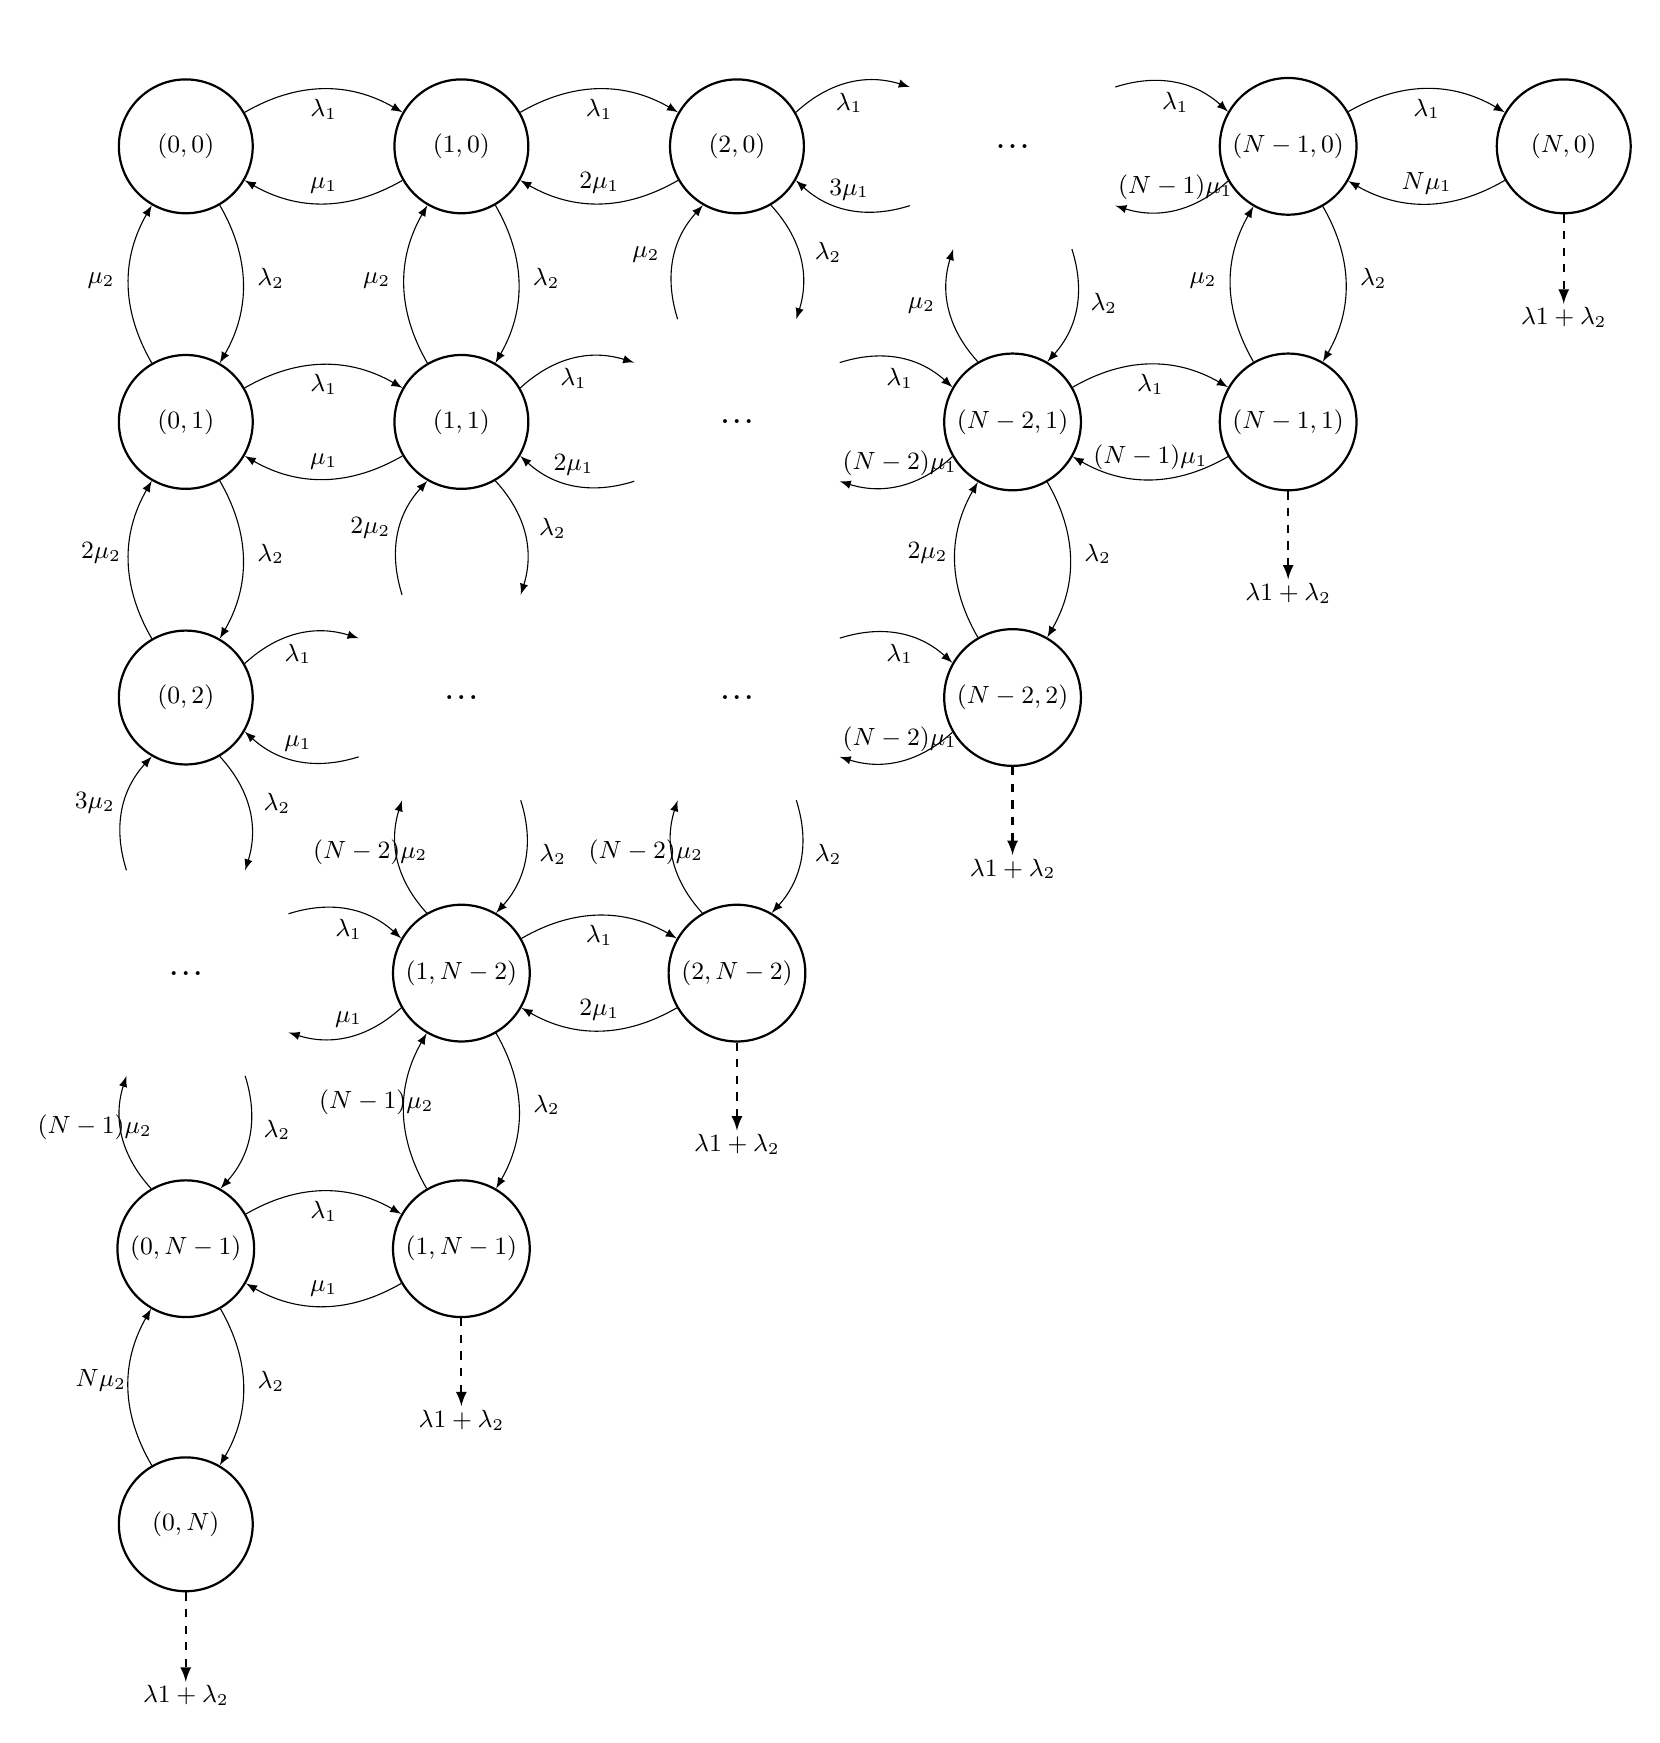
\begin{tikzpicture}[->,node distance=3.5cm,>=latex,font=\small, minimum width=1.7cm]

    \tikzstyle{round}=[thick,draw=black,circle]

    \node[round] 			    (00) {$(0,0)$};
    \node[round,right of=00]    (10) {$(1,0)$};
    \node[round,below of=00]    (01) {$(0,1)$};
    \node[round,below of=10]    (11) {$(1,1)$};
    \node[round,below of=01]    (02) {$(0,2)$};
    \node[round,right of=10]    (20) {$(2,0)$};
   
    \node[circle,draw=white,right of=20, minimum width = 3cm]    (A1) {\LARGE ...};
    \node[circle,draw=white,below of=02, minimum width = 3cm]    (A2) {\LARGE ...};
     
   	\node[round,right of=A1]    (N-1/0)  	{$(N-1,0)$};
   	\node[round,right of=N-1/0] (N0)	 	{$(N,0)$};
    \node[round,below of=N-1/0] (N-1/1)     {$(N-1,1)$};
    \node[round,left  of=N-1/1] (N-2/1)	{$(N-2,1)$};
    \node[round,below of=N-2/1] (N-2/2)	{$(N-2,2)$};
   
    \node[round,below of=A2]    (0/N-1)  	{$(0,N-1)$};
   	\node[round,below of=0/N-1] (0N)	 	{$(0,N)$};
    \node[round,right of=0/N-1] (1/N-1)     {$(1,N-1)$};
    \node[round,above of=1/N-1] (1/N-2)     {$(1,N-2)$};
    \node[round,right of=1/N-2] (2/N-2)	    {$(2,N-2)$};
    
    
    \node[circle,draw=white,left of=N-2/1,minimum width = 3cm]        (A3)     {\LARGE ...};
    \node[circle,draw=white,below of=11,minimum width = 3cm]          (A4)     {\LARGE ...};
    \node[circle,draw=white,above of=2/N-2,minimum width = 3cm]       (A5)     {\LARGE ...};
 
 	\draw[dashed,thick, ->] (N0) -- +(0,-2) node[yshift=-5]  {$\lambda1+\lambda_2$};
 	\draw[dashed,thick, ->] (N-1/1) -- +(0,-2) node[yshift=-5]  {$\lambda1+\lambda_2$};
 	\draw[dashed,thick, ->] (N-2/2) -- +(0,-2) node[yshift=-5]  {$\lambda1+\lambda_2$};
 	\draw[dashed,thick, ->] (2/N-2) -- +(0,-2) node[yshift=-5]  {$\lambda1+\lambda_2$};
 	\draw[dashed,thick, ->] (1/N-1) -- +(0,-2) node[yshift=-5]  {$\lambda1+\lambda_2$};
 	\draw[dashed,thick, ->] (0N) -- +(0,-2) node[yshift=-5]  {$\lambda1+\lambda_2$};
 
 	\path 
 	(00) 	edge[bend left,below]		node 					    {$\lambda_1$}		(10)
 		 	edge[bend left,above]       node [xshift=10,yshift=-5]  {$\lambda_2$} 		(01)
 	
 	(10) 	edge[bend left,above]       node 						{$\mu_1$} 			(00)
 		 	edge[bend left,below]		node 					    {$\lambda_1$}		(20)
 		 	edge[bend left,above]       node [xshift=10,yshift=-5]  {$\lambda_2$} 		(11)
 	
    (01) 	edge[bend left,above]       node [xshift=-10,yshift=-5] {$\mu_2$} 			(00)
   		 	edge[bend left,below]		node 					    {$\lambda_1$}		(11)
   	     	edge[bend left,above]       node [xshift=10,yshift=-5]  {$\lambda_2$} 		(02)
   
    (20) 	edge[bend left,above]       node 						{$2\mu_1$} 			(10)
    		edge[bend left,below]		node 					    {$\lambda_1$}		(A1)
    		edge[bend left,above]       node [xshift=10,yshift=-5]  {$\lambda_2$} 		(A3)
   		    
    (02) 	edge[bend left,above]       node [xshift=-10,yshift=-5] {$2\mu_2$} 			(01)
    		edge[bend left,above]       node [xshift=10,yshift=-5]  {$\lambda_2$} 		(A2)
    		edge[bend left,below]		node 					    {$\lambda_1$}		(A4)
   
    (11) 	edge[bend left,above]       node [xshift=-10,yshift=-5] {$\mu_2$} 			(10)
   		 	edge[bend left,above]       node 						{$\mu_1$} 			(01)
   		 	edge[bend left,below]		node 					    {$\lambda_1$}		(A3)
   		 	edge[bend left,above]       node [xshift=10,yshift=-5]  {$\lambda_2$} 		(A4)
   
   	(N0) 	edge[bend left,above]       node 						{$N\mu_1$} 			(N-1/0)
   
   	(N-1/0) edge[bend left,below]		node 					    {$\lambda_1$}		(N0)
   			edge[bend left,above]       node [xshift=10,yshift=-5]  {$\lambda_2$} 		(N-1/1)
   			edge[bend left,above]       node 						{$(N-1)\mu_1$} 			(A1)
   
    (N-1/1) edge[bend left,above]       node [xshift=-10,yshift=-5] {$\mu_2$} 			(N-1/0)
    		edge[bend left,above]       node 						{$(N-1)\mu_1$} 		(N-2/1)
    
    (N-2/1) edge[bend left,below]		node 					    {$\lambda_1$}		(N-1/1)
    		edge[bend left,above]       node [xshift=-10,yshift=-5] {$\mu_2$} 			(A1)
    		edge[bend left,above]       node 						{$(N-2)\mu_1$} 		(A3)
    		edge[bend left,above]       node [xshift=10,yshift=-5]  {$\lambda_2$} 		(N-2/2)
    		
    (N-2/2) edge[bend left,above]       node [xshift=-10,yshift=-5] {$2\mu_2$} 			(N-2/1)
    		edge[bend left,above]       node 						{$(N-2)\mu_1$} 		(A5)
    
    (0N) 	edge[bend left,above]       node [xshift=-10,yshift=-5]	{$N\mu_2$} 			(0/N-1)
   
   	(0/N-1) edge[bend left,below]		node 					    {$\lambda_1$}		(1/N-1)
   			edge[bend left,above]       node [xshift=10,yshift=-5]  {$\lambda_2$} 		(0N)
   			edge[bend left,above]       node [xshift=-10,yshift=-5]	{$(N-1)\mu_2$} 		(A2)
   
    (1/N-1) edge[bend left,above]       node 						{$\mu_1$}  			(0/N-1)
    	    edge[bend left,above]       node [xshift=-10,yshift=-5]	{$(N-1)\mu_2$} 		(1/N-2)
    
    (1/N-2) edge[bend left,above]       node 						{$\mu_1$}  			(A2)
    		edge[bend left,above]       node [xshift=10,yshift=-5]  {$\lambda_2$} 		(1/N-1)
    		edge[bend left,above]       node [xshift=-10,yshift=-5]	{$(N-2)\mu_2$} 		(A4)
    		edge[bend left,below]		node 					    {$\lambda_1$}		(2/N-2)
    		
    (2/N-2) edge[bend left,above]       node 						{$2\mu_1$}  		(1/N-2)
    		edge[bend left,above]       node [xshift=-10,yshift=-5]	{$(N-2)\mu_2$} 		(A5)
    
    (A1)    edge[bend left,above]       node 						{$3\mu_1$} 			(20)
    	    edge[bend left,below]		node 					    {$\lambda_1$}		(N-1/0)
    	    edge[bend left,above]       node [xshift=10,yshift=-5]  {$\lambda_2$} 		(N-2/1)
    	    
    (A2)	edge[bend left,above]       node [xshift=10,yshift=-5]  {$\lambda_2$} 		(0/N-1)
    		edge[bend left,above]       node [xshift=-10,yshift=-5]	{$3\mu_2$} 			(02)
    		edge[bend left,below]		node 					    {$\lambda_1$}		(1/N-2)
    		
    (A3)    edge[bend left,below]		node 					    {$\lambda_1$}		(N-2/1)
    		edge[bend left,above]       node [xshift=-10,yshift=-5]	{$\mu_2$} 			(20)
    		edge[bend left,above]       node 						{$2\mu_1$} 			(11)
    
    (A4)    edge[bend left,above]       node [xshift=-10,yshift=-5]	{$2\mu_2$} 			(11)
    		edge[bend left,above]       node 						{$\mu_1$} 			(02)
    		edge[bend left,above]       node [xshift=10,yshift=-5]  {$\lambda_2$} 		(1/N-2)
    		
    (A5)    edge[bend left,above]		node [xshift=10,yshift=-5]  {$\lambda_2$}		(2/N-2)
    		edge[bend left,below]		node 					    {$\lambda_1$}		(N-2/2);

\end{tikzpicture}
\end{adjustbox}
\end{figure}

Let's start with the analysis of the system when its routing policy is based on Algorithm \ref{alg:accessControlAlgorithm1}.

In order to compute all parameters and metrics of interest associated with that kind of system, we need to focus on  cloudlet node behaviour: since we know that, due to its limited resources, it can accept jobs until their number does not exceed a given threshold $N$, is crucial to firstly compute the \textit{fraction of jobs that are forwarded to cloudlet and to cloud}; in other word, from analytical point of view, our intent is to obtain the probability according to which the sum of job of each class in cloudlet node is equal to that threshold which can permit us to calculate fraction of jobs that are forwarded to each system's node.

To determine this probability, we have modelled cloudlet node as a \textit{continuous-time Markov chain} (CTMC) whose graphical representation is shown in Figure \ref{fig:ALG1-CloudletMarkovChain}; as you can see, each chain's state is denoted with $(n_1,n_2)$, where $n_1$ and $n_2$ represent respectively the number of class 1 and class 2 jobs.

\subsubsection{Balance equation} 

After have made CTMC modelling, we can compute \textit{limiting probabilities} $\pi_{(n_1,n_2)}$, namely the probability according to which the chain is in a certain state, say $j$, independently of the starting state, say $i$, via \textit{balance} (or \textit{stationary}) \textit{equations}, in which we can equate the rate at which the system leaves state $j$ with the rate at which the system enters state $j$ \footnote{Mor Harchol-Balter - \textit{Performance Modeling and Design of Computer Systems} - Carnegie Mellon University, Pennsylvania, page 237}, remembering that limiting probabilities sum to 1, that is $\sum_{j=0}^\infty \pi_j = 1$. Those balance equations are shown in table \ref{table:ALG1-CloudletBalanceEquationList}.


\begin{table}[h!]
    \caption{Balance equations.}
    \centering
    \small
    \begin{adjustbox}{center=\textwidth}
    \label{table:ALG1-CloudletBalanceEquationList}
     \begin{tabular}{rcll}

      \toprule

      $(\lambda_1 + \lambda_2)\pi_{(0,0)}$ & $=$ & $\mu_1\pi_{(1,0)} + \mu_2\pi_{(0,1)}$ \\\\
       
      $(\lambda_1 + \lambda_2 + n_1\mu_1)\pi_{(n_1,0)} $ & $=$ & $ \lambda_1\pi_{(n_1-1,0)} + \mu_1(n_1+1)\pi_{(n_1+1,0)} + \mu_2\pi_{(n_1,1)}$ & $\forall n_1 \in \mathbb{N} \cap [1, N-1]$ \\\\
      
      $(\lambda_1 + \lambda_2 + n_2\mu_2)\pi_{(0,n_2)} $ & $=$ & $ \lambda_2\pi_{(0,n_2-1)} + \mu_1\pi_{(1,n_2)} + \mu_2(n_2+1)\pi_{(0,n_2+1)}$ & $ \forall n_2 \in \mathbb{N} \cap [1, N-1]$ \\\\
      
      $\mu_1N\pi_{(N,0)}$ & $=$ & $\lambda_1\pi_{(N-1,0)}$ \\\\
      
      $\mu_2N\pi_{(0,N)}$ & $=$ & $\lambda_2\pi_{(0,N-1)}$ \\\\
      
      $(n_1\mu_1 + n_2\mu_2)\pi_{(n_1,n_2)} $ & $=$ & $ \lambda_1\pi_{(n_1-1,n_2)} + \lambda_2\pi_{(n_1,n_2-1)}$ & $\forall n_1,n_2 \in \mathbb{N} \cap [1, N-1] \mid n_1 + n_2 = N $ \\\\
      
      $(\lambda_1 + \lambda_2 + n_1\mu_1 + n_2\mu_2)\pi_{(n_1,n_2)} $ & $=$ & $ \lambda_1\pi_{(n_1-1,n_2)} + \lambda_2\pi_{(n_1,n_2-1)} + \mu_1(n_1+1)\pi_{(n_1+1,n_2)} $ & $\forall n_1,n_2 \in \mathbb{N} \cap [1, N-1] \mid n_1 + n_2 < N$\\
      && $+\; \mu_2(n_2+1)\pi_{(n_1,n_2+1)}$ & \\
      
      \bottomrule

    \end{tabular}
    \end{adjustbox}
\end{table}

Regarding balance equations resolution we have develop 

A Markov chain for which the limiting probabilities exist is said to be stationary or in steady state if the initial state is chosen according to the stationary probabilities. (page. 138)


\newpage
\subsubsection{Probabilities computing}

Having found the stationary probabilities, we can now find $\Pi_{\text{SendToCloud}}$, that is the \textit{probability that an arriving job on controller has to be forwarded to cloud}. Observe that the class to which an arrival job belongs to is not important because, according to access control Algorithm 1, jobs of both classes have same probability to be sent to cloud. To be more precise, \textbf{$\Pi_{\text{SendToCloud}}$} is the probability that an arrival job find that the number of jobs present in cloudlet has exceeded threshold $N$, which occurs when $n_1 + n_2 = N$. Formally:

\begin{equation}
\begin{array} {lcl} 
\Pi_{\text{SendToCloud}} & = & P\lbrace{\text{An arrival job on controller sees $N$ jobs in cloudlet}}\rbrace \\\\

& = & \text{Limiting probability that there are $N$ jobs in system} \\\\

& = & \displaystyle \sum_{\substack{n_1, n_2 \in \mathbb{N} \cap [0, N] \\ n1+n2=N}} \pi_{(n_1,n_2)} \\
\end{array}
\end{equation}

At this point we can easily compute \textbf{$\Pi_{\text{SendToCloudlet}}$}, which instead represents the \textbf{probability according to which an arriving job on controller has to be accepted on cloudlet} and it is same for both job classes too.

\begin{equation}
\begin{array} {lcl} 
\Pi_{\text{SendToCloudlet}} & = & P\lbrace{\text{An arrival job on controller sees less than $N$ jobs in cloudlet}}\rbrace \\\\
& = & 1 - P\lbrace{\text{An arrival job on controller sees $N$ jobs in cloudlet}}\rbrace \\\\

& = & 1 - \Pi_{\text{SendToCloud}} \\\\
\end{array}
\end{equation}

\subsubsection{Average arrival rates}

Is $\lambda_x^{(c)}$ the \textit{total arrival rate into a system's component $x$ of class $c$ job}. Applying previous results, using an appropriate equation\footnote{\textit{Cfr.} \textit{Ibid.}, page 315, equation (18.1)}, we can now compute per-class average arrival rates as follow:

\begin{equation}
\begin{array} {rcl}

\lambda_{\text{cloud}}^{(1)} & = & \lambda_1\cdot \Pi_{\text{SendToCloud}} \\\\
\lambda_{\text{cloud}}^{(2)} & = & \lambda_2\cdot \Pi_{\text{SendToCloud}} \\\\
\lambda_{\text{cloudlet}}^{(1)} & = & \lambda_1\cdot \Pi_{\text{SendToCloudlet}} \\\\
\lambda_{\text{cloudlet}}^{(2)} & = & \lambda_2\cdot \Pi_{\text{SendToCloudlet}} \\\\
\end{array}
\end{equation}

Then we get $\lambda_i$, that is \textbf{total arrival rate to system's component $i$}, by summing the per-class rates as follows:

\begin{equation}
\begin{array} {rcl}
\lambda_{\text{cloud}} & = & \lambda_{\text{cloud}}^{(1)} + \lambda_{\text{cloud}}^{(2)} \\\\
\lambda_{\text{cloudlet}} & = & \lambda_{\text{cloudlet}}^{(1)} + \lambda_{\text{cloudlet}}^{(2)} \\\\
\end{array}
\end{equation}


\subsubsection{Average population}

Is $E[N_x]^{(c)}$ the time-average population of class $c$ jobs into a system's node $x$. 

We can use previously computed stationary probabilities to get average population for cloudlet; it's enough to sum each state's limiting probability multiplied by corresponding number of job as follows:

\begin{equation}
\label{eq:cloudletAveragePopulation}
\begin{array} {rcl} 
E[N_{\text{cloudlet}}^{(1)}] & = & \displaystyle \sum_{ (n_1, n_2) \in M} n_1 \cdot \pi_{(n_1,n_2)}  \\\\

E[N_{\text{cloudlet}}^{(2)}] & = & \displaystyle \sum_{ (n_1, n_2) \in M} n_2 \cdot \pi_{(n_1,n_2)}  \\\\

E[N_{\text{cloudlet}}] & = & E[N_{\text{cloudlet}}^{(1)}] + E[N_{\text{cloudlet}}^{(2)}] \\\\

& = & \displaystyle \sum_{ (n_1, n_2) \in M} (n_1 + n_2) \cdot \pi_{(n_1,n_2)} \\\\

\end{array}
\end{equation}

Since we have modelled cloud component as a $M/M/\infty$ system, in which there is no job's waiting time due to presence of an infinite number of servers, we can simply to apply \textbf{Little’s Law}\footnote{\textit{Ibid.}, pag. 95, theorem (6.1)} in order to get cloud's average population as shown in Equation \ref{equation:ALG-1}.

\begin{equation}
\label{eq:cloudAveragePopulation1}
\begin{array} {rcl} 
E[N_{\text{cloud}}^{(1)}] & = & \lambda_{\text{cloud}}^{(1)} \cdot E[T_{\text{cloud}}^{(1)}]  \\\\

& = & \lambda_{\text{cloud}}^{(1)} \cdot (E[T_{Q_{\text{cloud}}}^{(1)}] + E[S_{\text{cloud}}^{(1)}])  \\\\

& = & \lambda_{\text{cloud}}^{(1)} \cdot (\frac{1}{\mu_{\text{cloud}}^{(1)}}) \\\\

& = & \dfrac{\lambda_{\text{cloud}}^{(1)}}{\mu_{\text{cloud}}^{(1)}} \\

\end{array}
\end{equation}

Similarly:
 
\begin{equation}
\label{eq:cloudAveragePopulation2}
\begin{array} {rcl} 
E[N_{\text{cloud}}^{(2)}] & = & \dfrac{\lambda_{\text{cloud}}^{(2)}}{\mu_{\text{cloud}}^{(2)}}
\end{array}
\end{equation}

\begin{equation}
\label{eq:cloudAveragePopulation3}
\begin{array} {rcl} 
E[N_{\text{cloud}}] & = & E[N_{\text{cloud}}^{(1)}] + E[N_{\text{cloud}}^{(2)}]
\end{array}
\end{equation}

Finally we can get global average job populations as follows:

\begin{equation}
\label{eq:AveragePopulation}
\begin{array} {rcl} 

E[N^{(1)}] & = & E[N_{\text{cloudlet}}^{(1)}] + E[N_{\text{cloud}}^{(1)}] \\\\

E[N^{(2)}] & = & E[N_{\text{cloudlet}}^{(2)}] + E[N_{\text{cloud}}^{(2)}] \\\\

E[N] & = & E[N^{(1)}] + E[N^{(2)}]

\end{array}
\end{equation}


\subsubsection{Average response time}

Is $E[T_x^{(c)}]$ the \textit{mean response time experienced by a class $c$ jobs into a component $x$}. 

In order to properly compute said metric for each system's component observe that:
\begin{itemize}
\item Knowing per-class average job population and per-class mean arrival rates, we can easily compute $E[T_x^{(c)}]$ using Little’s Law.
\item Since our system haven't queues, no waiting time is experienced by jobs, therefore is true that $E[T_x^{(c)}]$ is also equal to $E[S_x^{(c)}]$, that is \textit{mean service time experienced by a class $c$ jobs into a component $x$}, which is equal to $1/\mu_x^{(c)}$, where $\mu_x^{(c)}$ means average service rate at which a class $c$ jobs into a component $x$ is served.
\end{itemize}

Therefore we can get these metric as follows.

\begin{equation}
\begin{array} {rcl} 
E[T_{\text{cloudlet}}^{(1)}] & = & \dfrac{E[N_{\text{cloudlet}}^{(1)}]}{\lambda_{\text{cloudlet}}^{(1)}} \\\\

& = & E[S_{\text{cloudlet}}^{(1)}] \\\\

& = & \dfrac{1}{\mu_{\text{cloudlet}}^{(1)}} \\\\
\end{array}
\end{equation}

\begin{equation}
\begin{array} {rcl} 
E[T_{\text{cloudlet}}^{(2)}] & = & \dfrac{E[N_{\text{cloudlet}}^{(2)}]}{\lambda_{\text{cloudlet}}^{(2)}} \\\\

& = & E[S_{\text{cloudlet}}^{(2)}] \\\\

& = & \dfrac{1}{\mu_{\text{cloudlet}}^{(2)}} \\\\
\end{array}
\end{equation}

\begin{equation}
\begin{array} {rcl} 
E[T_{\text{cloud}}^{(1)}] & = & \dfrac{E[N_{\text{cloud}}^{(1)}]}{\lambda_{\text{cloud}}^{(1)}} \\\\

& = & E[S_{\text{cloud}}^{(1)}] \\\\

& = & \dfrac{1}{\mu_{\text{cloud}}^{(1)}} \\\\
\end{array}
\end{equation}

\begin{equation}
\begin{array} {rcl} 
E[T_{\text{cloud}}^{(2)}] & = & \dfrac{E[N_{\text{cloud}}^{(2)}]}{\lambda_{\text{cloud}}^{(2)}} \\\\

& = & E[S_{\text{cloud}}^{(2)}] \\\\

& = & \dfrac{1}{\mu_{\text{cloud}}^{(2)}} \\\\
\end{array}
\end{equation}

At this point we can get global per-class mean response times as follows:

\begin{equation}
\begin{array} {lcl} 
E[T^{(1)}] & = & E[T_{\text{cloudlet}}^{(1)}] \cdot P\lbrace\text{An arrival class 1 job is sent to cloudlet}\rbrace \\
\\
& & +\; E[T_{\text{cloud}}^{(1)}] \cdot P\lbrace\text{An arrival class 1 job is sent to cloud}\rbrace \\
\\
& = & E[T_{\text{cloudlet}}^{(1)}] \cdot \Pi_{\text{SendToCloudlet}} + E[T_{\text{cloud}}^{(1)}] \cdot \Pi_{\text{SendToCloud}} \\

\end{array}
\end{equation}

Similarly:

\begin{equation}
\begin{array} {lcl} 
E[T^{(2)}] & = & E[T_{\text{cloudlet}}^{(2)}] \cdot P\lbrace\text{An arrival class 2 job is sent to cloudlet}\rbrace \\
\\
& & +\; E[T_{\text{cloud}}^{(2)}] \cdot P\lbrace\text{An arrival class 2 job is sent to cloud}\rbrace \\
\\
& = & E[T_{\text{cloudlet}}^{(2)}] \cdot \Pi_{\text{SendToCloudlet}} + E[T_{\text{cloud}}^{(2)}] \cdot \Pi_{\text{SendToCloud}} \\

\end{array}
\end{equation}

Finally, using obtained results, we can get global mean response times as shown below:

\begin{equation}
E[T] = E[T^{(1)}] \cdot \dfrac{\lambda_1}{\lambda_1 + \lambda_2} + E[T^{(2)}] \cdot \dfrac{\lambda_2}{\lambda_1 + \lambda_2}
\end{equation}

\subsubsection{Throughput}

To determine system's throughput let's prove if our system is stable.
As we know, every queueing system in which its mean arrival rate is less than its mean service rate is known as a stable system; formally, are $\lambda$ and $\mu$ our system's mean arrival rate and mean service rate respectively, if $\lambda \leq \mu$, given system is stable.
Cloudlet subsystem is clearly \textit{not} stable due to its limited resources compared to its workload; we have already seen that exists a not null probability according to which an arriving job on controller sees $N$ jobs in cloudlet which implying its forward to cloud subsystem. Since it haven't a queue, cloudlet stability condition is achieved when $\Pi_{\text{SendToCloud}}$ is null but, based on current system parameters, is not the case.
Regarding cloud subsystem, no matter how high we make $\lambda_{\text{cloud}}$ because it is made up of an infinite number of server for which completion rate is still bounded by the arrival rate.
Accordingly to previous considerations we can conclude that \textbf{our system is stable} due to stability or its cloud subsystem therefore we can get system throughput as follows:

\begin{equation}
X = \lambda = \lambda_1 + \lambda_2 \\
\end{equation}

To get per-subsystems throughput we proceed as shown below:

\begin{equation}
X_{\text{cloud}} = \lambda_{\text{cloud}} \\
\end{equation}

\begin{equation}
X_{\text{cloudlet}} = X - X_{\text{cloud}} \\
\end{equation}


\newpage

\begin{figure}[h!]
\caption{Cloudlet system component modeled using a CTMC} \label{fig:ALG2-CloudletMarkovChain}
\begin{adjustbox}{center=\textwidth}
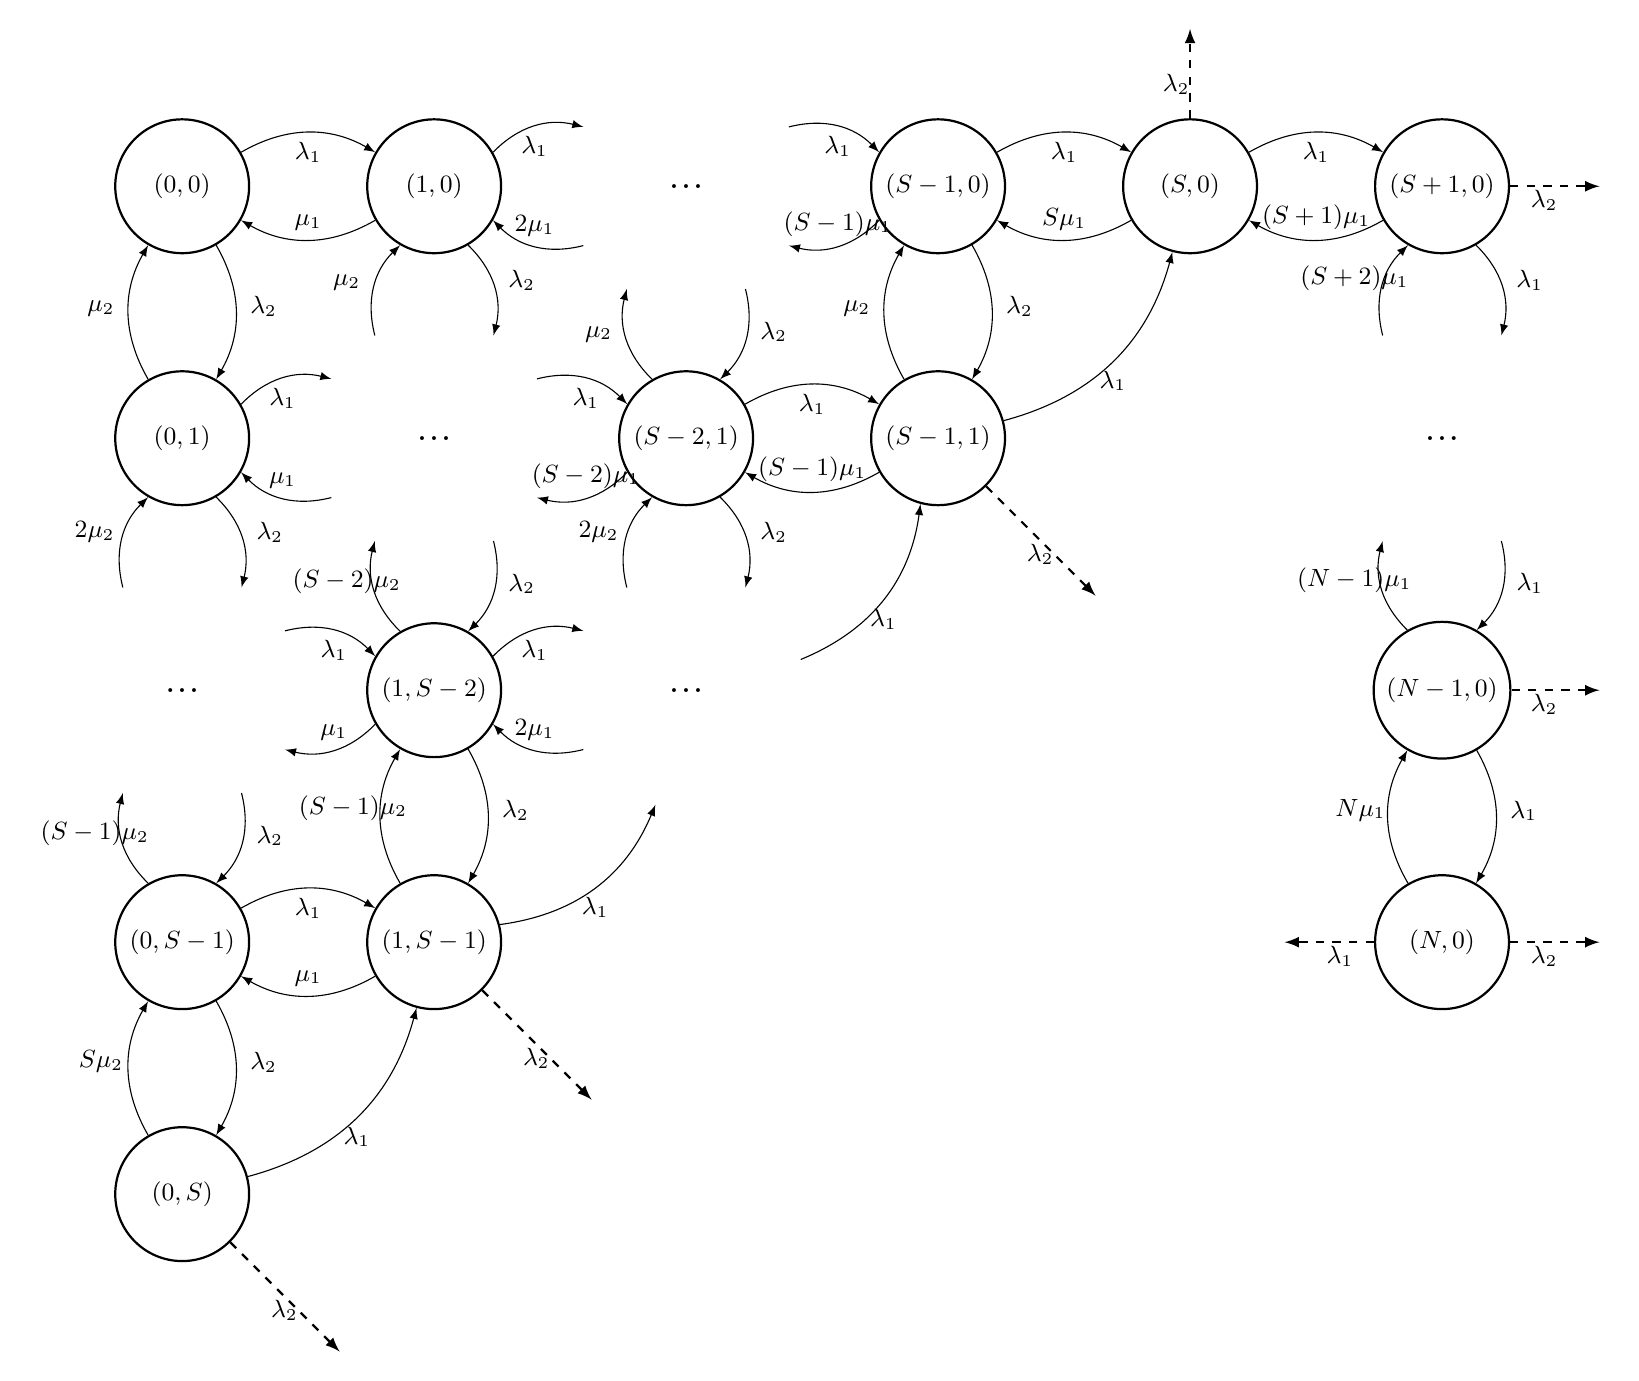
\begin{tikzpicture}[->,node distance=3.2cm,>=latex,font=\small, minimum width=1.7cm]

    \tikzstyle{round}=[thick,draw=black,circle]

    \node[round] 			    (00) {$(0,0)$};
    \node[round,right of=00]    (10) {$(1,0)$};
    \node[round,below of=00]    (01) {$(0,1)$};
    
	\node[circle,draw=white,right of=10, minimum width = 3cm]    (B0) {\LARGE ...};
    \node[circle,draw=white,below of=01, minimum width = 3cm]    (B1) {\LARGE ...};    
    
   	\node[round,right of=B0]    (S-1/0)  	{$(S-1,0)$};
   	\node[round,right of=S-1/0] (S0)	 	{$(S,0)$};
    \node[round,below of=S-1/0] (S-1/1)     {$(S-1,1)$};
    \node[round,left  of=S-1/1] (S-2/1)	{$(S-2,1)$};
   
    \node[round,below of=B1]    (0/S-1)  	{$(0,S-1)$};
   	\node[round,below of=0/S-1] (0S)	 	{$(0,S)$};
    \node[round,right of=0/S-1] (1/S-1)     {$(1,S-1)$};
    \node[round,above of=1/S-1] (1/S-2)     {$(1,S-2)$};
    
    
    \node[circle,below of=10, minimum width = 3cm]    (B2) {\LARGE ...};
    \node[circle,draw=white,right of=1/S-2, minimum width = 3cm]    (B3) {\LARGE ...};
   
    \node[round,right of=S0] (S+1/0)	 	{$(S+1,0)$};  
    \node[circle,draw=white,below of=S+1/0, minimum width = 3cm]    (B4) {\LARGE ...};
    \node[round,below of=B4] (N-1/0)	 	{$(N-1,0)$};  
    \node[round,below of=N-1/0] (N0)	 	{$(N,0)$};  
   
    \draw[dashed,thick, ->] (N0) -- +(2,0) node[xshift=-20,yshift=-5]  {$\lambda_2$};
    \draw[dashed,thick, ->] (N0) -- +(-2,0) node[xshift=20,yshift=-5]  {$\lambda_1$};
    
    \draw[dashed,thick, ->] (N-1/0) -- +(2,0) node[xshift=-20,yshift=-5]  {$\lambda_2$};
    \draw[dashed,thick, ->] (S+1/0) -- +(2,0) node[xshift=-20,yshift=-5]  {$\lambda_2$};
    \draw[dashed,thick, ->] (S0) -- +(0,2) node[xshift=-5,yshift=-20]  {$\lambda_2$};
    \draw[dashed,thick, ->] (1/S-1) -- +(2,-2) node[xshift=-20,yshift=15]  {$\lambda_2$};
    \draw[dashed,thick, ->] (S-1/1) -- +(2,-2) node[xshift=-20,yshift=15]  {$\lambda_2$};
    \draw[dashed,thick, ->] (0S) -- +(2,-2) node[xshift=-20,yshift=15]  {$\lambda_2$};
   
 	\path 
 	
 	(S+1/0)edge[bend left,above]    node {$(S+1)\mu_1$} 		(S0)
 		   edge[bend left,above]       node [xshift=10,yshift=-5]  {$\lambda_1$} 		(B4)
 	
 	(B4)   edge[bend left,above]       node [xshift=-10,yshift=-5] {$(S+2)\mu_1$} 		(S+1/0)
 		   edge[bend left,above]       node [xshift=10,yshift=-5]  {$\lambda_1$} 		(N-1/0)
 		   
 		   
 	(N-1/0)	 edge[bend left,above]       node [xshift=10,yshift=-5]  {$\lambda_1$} 		(N0)
 			 edge[bend left,above]       node [xshift=-10,yshift=-5] {$(N-1)\mu_1$} 	(B4)
 		   
    (N0) edge[bend left,above]       node [xshift=-10,yshift=-5] {$N\mu_1$} 		(N-1/0)
 	
 	(00) 	edge[bend left,below]		node 					    {$\lambda_1$}		(10)
 		 	edge[bend left,above]       node [xshift=10,yshift=-5]  {$\lambda_2$} 		(01)
 	
 	(10) 	edge[bend left,above]       node 						{$\mu_1$} 			(00)
 		 	edge[bend left,below]		node 					    {$\lambda_1$}		(B0)
 		 	edge[bend left,above]       node [xshift=10,yshift=-5]  {$\lambda_2$} 		(B2)
 	
    (01) 	edge[bend left,above]       node [xshift=-10,yshift=-5] {$\mu_2$} 			(00)
   		 	edge[bend left,below]		node 					    {$\lambda_1$}		(B2)
   	     	edge[bend left,above]       node [xshift=10,yshift=-5]  {$\lambda_2$} 		(B1)
   
    (B0) 	edge[bend left,above]       node 						{$2\mu_1$} 			(10)
    		edge[bend left,above]       node [xshift=10,yshift=-5]  {$\lambda_2$} 		(S-2/1)
    		edge[bend left,below]		node 					    {$\lambda_1$}		(S-1/0)
   		    
    (B1) 	edge[bend left,above]       node [xshift=-10,yshift=-5] {$2\mu_2$} 			(01)
   			edge[bend left,above]       node [xshift=10,yshift=-5]  {$\lambda_2$} 		(0/S-1)
   			edge[bend left,below]		node 					    {$\lambda_1$}		(1/S-2)
   			
   
    (B2) 	edge[bend left,above]       node [xshift=-10,yshift=-5] {$\mu_2$} 			(10)
   		 	edge[bend left,above]       node 						{$\mu_1$} 			(01)
   		 	edge[bend left,above]       node [xshift=10,yshift=-5]  {$\lambda_2$} 		(1/S-2)
   		 	edge[bend left,below]		node 					    {$\lambda_1$}		(S-2/1)
   		 	
    (B3)    edge[bend left,above]       node [xshift=-10,yshift=-5] {$2\mu_2$} 			(S-2/1)
   		    edge[bend left,above]       node 						{$2\mu_1$} 			(1/S-2)   	
   		    edge[bend right,below]		node 					    {$\lambda_1$}		(S-1/1)	 	
   		 	
    (S0) 	edge[bend left,above]       node 						{$S\mu_1$} 			(S-1/0)
 			 edge[bend left,below]		node 					    {$\lambda_1$}		(S+1/0)	
 			 
   	(S-1/0) edge[bend left,below]		node 					    {$\lambda_1$}		(S0)
   			edge[bend left,above]       node [xshift=10,yshift=-5]  {$\lambda_2$} 		(S-1/1)
   			edge[bend left,above]       node 						{$(S-1)\mu_1$} 		(B0)
   
    (S-1/1) edge[bend left,above]       node [xshift=-10,yshift=-5] {$\mu_2$} 			(S-1/0)
    		edge[bend left,above]       node 						{$(S-1)\mu_1$} 		(S-2/1)
    		edge[bend right,below]		node 					    {$\lambda_1$}		(S0)	 
    
    (S-2/1) edge[bend left,below]		node 					    {$\lambda_1$}		(S-1/1)
    		edge[bend left,above]       node [xshift=-10,yshift=-5] {$\mu_2$} 			(B0)
    		edge[bend left,above]       node 						{$(S-2)\mu_1$} 		(B2)
    		edge[bend left,above]       node [xshift=10,yshift=-5]  {$\lambda_2$} 		(B3)
		 
    (0S) 	edge[bend left,above]       node [xshift=-10,yshift=-5]	{$S\mu_2$} 			(0/S-1)
    		edge[bend right,below]		node 					    {$\lambda_1$}		(1/S-1)
   
   	(0/S-1) edge[bend left,below]		node 					    {$\lambda_1$}		(1/S-1)
   			edge[bend left,above]       node [xshift=10,yshift=-5]  {$\lambda_2$} 		(0S)
   			edge[bend left,above]       node [xshift=-10,yshift=-5]	{$(S-1)\mu_2$} 		(B1)
   
    (1/S-1) edge[bend left,above]       node 						{$\mu_1$}  			(0/S-1)
    	    edge[bend left,above]       node [xshift=-10,yshift=-5]	{$(S-1)\mu_2$} 		(1/S-2)
    	    edge[bend right,below]		node 					    {$\lambda_1$}		(B3)
    
    (1/S-2) edge[bend left,above]       node 						{$\mu_1$}  			(B1)
    		edge[bend left,above]       node [xshift=10,yshift=-5]  {$\lambda_2$} 		(1/S-1)
    		edge[bend left,above]       node [xshift=-10,yshift=-5]	{$(S-2)\mu_2$} 		(B2)
    		edge[bend left,below]		node 					    {$\lambda_1$}		(B3)
  
    		
   ;
  
\end{tikzpicture}
\end{adjustbox}
\end{figure}

\newpage
\subsection{System based on access control Algorithm 2}

Based on our analysis, performance achieved by our system when its routing policy is based on second algorithm, reported in Algorithm \ref{alg:accessControlAlgorithm2}, are very different from previous case. 

The main feature of this kind of system is that a class 2 job, running on cloudlet, may be stopped through its execution on system's cloudlet node and then subsequently resumed in system's cloud node; is important to specify that adopted routing policy is \textit{not} work-conserving because it re-runs interrupted jobs losing work previously done. Moreover, when a class 2 job is interrupted and sent on the system's cloud node, a setup time, denoted whit $s_{setup}$, has to be considered to restart the task on the cloud. 

Most equations described and used in section \ref{subsub:alg1} are still valid also for this system, although there are differences about numerical values of each metrics; therefore in this section we focus only to differences compared to previous case.

\subsubsection{Balance equation}

Regarding balance equation necessary for stationary probabilities computation, since there are no differences about mathematical notation used or significant conceptual differences compared to previously case, we limit ourselves to report them in table \ref{table:ALG2-CloudletBalanceEquationList}.

\begin{table}[h!]
    \caption{Balance equations.}
    \centering
    \small
    \begin{adjustbox}{center=\textwidth}
    \label{table:ALG2-CloudletBalanceEquationList}
     \begin{tabular}{rcll}

      \toprule

      $(\lambda_1 + \lambda_2)\pi_{(0,0)}$ & $=$ & $\mu_1\pi_{(1,0)} + \mu_2\pi_{(0,1)}$ \\\\
       
      $(\lambda_1 + \lambda_2 + n_1\mu_1)\pi_{(n_1,0)} $ & $=$ & $ \lambda_1\pi_{(n_1-1,0)} + \mu_1(n_1+1)\pi_{(n_1+1,0)} + \mu_2\pi_{(n_1,1)}$ & $\forall n_1 \in \mathbb{N} \cap [1, S-1]$ \\\\
      
      $(\lambda_1 + \lambda_2 + n_2\mu_2)\pi_{(0,n_2)} $ & $=$ & $ \lambda_2\pi_{(0,n_2-1)} + \mu_1\pi_{(1,n_2)} + \mu_2(n_2+1)\pi_{(0,n_2+1)}$ & $ \forall n_2 \in \mathbb{N} \cap [1, S-1]$ \\\\
      
      $(S\mu_1+\lambda_1)\pi_{(S,0)}$ & $=$ & $\lambda_1\pi_{(S-1,0)} + \lambda_1\pi_{(S-1,1)} + (S+1)\mu_1 \pi_{(S+1,0)}$ \\\\
      
      $(\lambda_1 + S\mu_2) \pi_{(0,S)}$ & $=$ & $\lambda_2\pi_{(0,S-1)}$ \\\\
      
      $(n_1\mu_1 + n_2\mu_2 + \lambda_1)\pi_{(n_1,n_2)} $ & $=$ & $ \lambda_1\pi_{(n_1-1,n_2+1)} + \lambda_1\pi_{(n_1-1,n_2)} + \lambda_2\pi_{(n_1,n_2-1)}$ & $\forall n_1,n_2 \in \mathbb{N} \cap [1, S-1] \mid n_1 + n_2 = S $ \\\\
      
      $(\lambda_1 + \lambda_2 + n_1\mu_1 + n_2\mu_2)\pi_{(n_1,n_2)} $ & $=$ & $ \lambda_1\pi_{(n_1-1,n_2)} + \lambda_2\pi_{(n_1,n_2-1)} + \mu_1(n_1+1)\pi_{(n_1+1,n_2)} $ & $\forall n_1,n_2 \in \mathbb{N} \cap [1, S-1] \mid n_1 + n_2 < S$\\
      && $+\; \mu_2(n_2+1)\pi_{(n_1,n_2+1)}$ & \\\\
      
      $(n_1\mu_1 + \lambda_1)\pi_{(n_1,0)}$ & = & $\mu_1(n_1+1)\pi_{(n_1+1,0)} + \lambda_1\pi_{(n_1-1,0)}$ & $\forall n_1 \in \mathbb{N} \mid S+1 \leq n_1 \leq N-1$ \\\\

      $N\mu_1\pi_{(N,0)}$ & = & $\lambda_1\pi_{(N-1,0)}$ \\
      
      \bottomrule

    \end{tabular}
    \end{adjustbox}
\end{table}

\newpage
\subsubsection{Probabilities computing}

Let's start clarifying all differences, compared to previous case, about routing probabilities necessary for analytical results computations.

Is $\Pi_{\text{SendToCloud}}^{(c)}$ the probability according to which an arriving class $c$ job on controller has to be forwarded to system's cloud node. Observing both CTMC and routing policy algorithm is very easy to understand that:

\begin{equation}
\begin{array} {lcl} 
\Pi_{\text{SendToCloud}}^{(1)} & = & P\lbrace\text{An arrival class 1 job on controller sees $N$ class 1 jobs in cloudlet.}\rbrace \\ 
\\
& = & P\lbrace{n_1 = N}\rbrace \\ 
\\
& = & \pi_{(N,0)}
\end{array}
\end{equation}


\begin{equation}
\begin{array} {lcl} 
\Pi_{\text{SendToCloud}}^{(2)} & = & P \bigg\{ \begin{array}{l} \text{An arrival class 2 job on controller sees that number of} \\ \text{jobs in cloudlet exceed or is equal to a given threshold $S$.} \end{array} \bigg\} \\
\\
& = & P\lbrace{n_1 + n_2 \geq S}\rbrace \\ 
\\
& = & \displaystyle \sum_{\substack{0 \leq n_1 \leq S \\ 0 \leq n_2 \leq S \\ n_1 + n_2 = S}} \pi_{(n_1,n_2)} + \sum_{n_1 = S+1}^{N}\pi_{(n_1,0)} \\
\\
& = & \displaystyle \sum_{\substack{0 \leq n_1 \leq N \\ 0 \leq n_2 \leq S \\ n_1 + n_2 \geq S}} \pi_{(n_1,n_2)}\\
\end{array}
\end{equation}

Is $\Pi_{\text{SendToCloudlet}}^{(c)}$ the probability that an arriving class $c$ job on controller has to be forwarded to system's cloudlet node. 

In order to compute these probabilities we can proceed as shown below:

\begin{equation}
\begin{array} {lcl} 
\Pi_{\text{SendToCloudlet}}^{(1)} & = & 1 - \Pi_{\text{SendToCloud}}^{(1)} \\
\\
\Pi_{\text{SendToCloudlet}}^{(2)} & = & 1 - \Pi_{\text{SendToCloud}}^{(2)} \\
\end{array}
\end{equation}

To compute $\Pi_{\text{interruption}}^{(2)}$, that is the probability according to which a class 2 job, running on cloudlet, have to be stopped and forwarded to system's cloud node, is necessary know firstly $\Pi_{\text{interruptible}}$, the probability that system's cloudlet node is in a state in which any future class 1 job arrival is able to cause a class 2 job interruption. Formally:

\begin{equation}
\begin{array} {lcl} 
\Pi_{\text{interruptible}} & = & P \bigg\{ \begin{array}{l} \text{System's cloudlet node is in a state in which any future class} \\ \text{1 job arrival is able to cause a class 2 job interruption.} \end{array} \bigg\} \\
\\
& = & P\lbrace{n_1 + n_2 = S, n_2 > 0}\rbrace \\ 
\\
& = & \displaystyle \sum_{\substack{0 \leq n_1 \leq S-1 \\ 1 \leq n_2 \leq S \\ n_1 + n_2 = S}} \pi(n_1,n_2) \\
\\
\end{array}
\end{equation}

At this point we can formally define $\Pi_{\text{interruption}}^{(2)}$ as follows:

\begin{equation}
\begin{array} {lcl} 
\Pi_{\text{interruption}}^{(2)} & = & P \Bigg\{ \begin{array}{l} \text{A class 1 job is forwarded to system's cloudlet node when} \\ \text{it is in a state in which any class 1 job arrival is able to} \\ \text{cause a class 2 job interruption.} \end{array} \Bigg\} \\
\\
& = & P \Bigg\{ \Bigg( \begin{array}{l} \text{System's cloudlet node is in a} \\ \text{state in which any future class} \\ \text{1 job arrival is able to cause a} \\ \text{class 2 job interruption.} \end{array} \Bigg) \cap \Bigg( \begin{array}{l} \text{A class 1 job is forwarded} \\ \text{to system's cloudlet node.} \end{array} \Bigg) \Bigg\} \\
\\
& = & \Pi_{\text{interruptible}} \cdot \Pi_{\text{SendToCloudlet}}^{(1)}\\
\\
\end{array}
\end{equation}

\subsubsection{Average arrival rates}

Finally, applying previous results, we can now compute per-class average arrival rates as follow of our system:

\begin{equation}
\begin{array} {rcl}

\lambda_{\text{cloud}}^{(1)} & = & \lambda_1\cdot \Pi_{\text{SendToCloud}}^{(1)} \\\\
\lambda_{\text{cloud}}^{(2)} & = & \lambda_2\cdot \Pi_{\text{SendToCloud}}^{(2)} \\\\
\lambda_{\text{cloudlet}}^{(1)} & = & \lambda_1\cdot \Pi_{\text{SendToCloudlet}}^{(1)} \\\\
\lambda_{\text{cloudlet}}^{(2)} & = & \lambda_2\cdot \Pi_{\text{SendToCloudlet}}^{(2)} \\\\
\end{array}
\end{equation}

Then we can get $\lambda_x$, that is total arrival rate to system's component $x$, proceeding as follows:

\begin{equation}
\begin{array} {rcl}

\lambda_{\text{cloud}} & = & \lambda_{\text{cloud}}^{(1)} + \lambda_{\text{cloud}}^{(2)} + \lambda_{\text{cloudlet}}^{(2)} \cdot \Pi_{\text{interruption}}^{(2)} \\\\

\lambda_{\text{cloudlet}} & = & \lambda_{\text{cloudlet}}^{(1)} + \lambda_{\text{cloudlet}}^{(2)} \\
\end{array}
\end{equation}

\subsubsection{Other metrics}

In order to compute $E[N_x]^{(c)}$ and $E[T_x]^{(c)}$, respectively averaged population and response time of class $c$ jobs running in a $x$ system's node, is possible to use same equations described in previous section because, although stationary probabilities and arrival rates have different numeric values, due to different routing policy, there are no conceptual differences about computation of those metrics.

Analytical methods used to compute system throughput are pretty the same as those used in previous section. The only difference lies in cloudlet class 2 throughput  $X_{\text{cloudlet}}^{(2)}$ computation, computable using equation shown below:

\begin{equation}
\begin{array} {lcl} 
X_{\text{cloudlet}}^{(2)} & = & \lambda_{\text{cloudlet}}^{(2)} - \lambda_{\text{cloudlet}}^{(2)} \cdot \Pi_{\text{interruption}}^{(2)}
\end{array}
\end{equation}

Regarding instead $E[T]^{(2)}$, that is global averaged response time experienced by class 2 jobs, there are, instead, some conceptual differences due to jobs interruptions. Formally:


\begin{equation}
\begin{array} {lcl} 
E[T]^{(2)}  & = & \Pi_{\text{SendToCloud}}^{(2)} \cdot E[T_{\text{cloud}}^{(2)}] \; +  \\
& & \Pi_{\text{SendToCloudlet}}^{(2)} \cdot \bigg( \Pi_{\text{interruption}}^{(2)}\cdot(E[S_{setup}] + E[T_{\text{cloud}}^{(2)}]) + (1-\Pi_{\text{interruption}}^{(2)}) \cdot E[T_{\text{cloudlet}}^{(2)}] \bigg)
\end{array}
\end{equation}

Finally, in order to compute average response time relating to interrupted class 2 jobs only, denoted with $E[T]^{(2)}_{\text{interrupted}}$, we can simply proceed as shown below:

\begin{equation}
\begin{array} {lcll} 
E[T]^{(2)}_{\text{interrupted}}  & = & E[S_{\text{setup}}] + E[T_{\text{cloud}}^{(2)}] + \alpha \cdot E[T_{\text{cloudlet}}^{(2)}] & \quad \forall \alpha \in \mathbb{R} \mid 0 \leq \alpha \leq 1
\end{array}
\end{equation}

In order to compute the fraction of time during which interrupted class 2 job was running on the cloudlet, we have used an attenuation factor $\alpha$ which value, determined experimentally, is equal to $0.649$.


\newpage
\subsection{Summary of analytical results}


All analytical results are been computed using a combination of Java and MATLAB\footnote{See. \texttt{https://www.mathworks.com/products/matlab.html}} scripts.

In fact, all balance equations, previously shown in tables \ref{table:ALG1-CloudletBalanceEquationList} and \ref{table:ALG2-CloudletBalanceEquationList}, are firstly automatically generated using simple Java scripts\footnote{See \texttt{CTMCResolverScriptGenerator.java}, \texttt{ResolverUsingRoutingAlgorithm1.java} and \texttt{ResolverUsingRoutingAlgorithm2.java} files.} able to built some MATLAB scripts as output\footnote{See \texttt{MATLAB\_ALG1\_CTMC\_ResolverScript.m} and \texttt{MATLAB\_ALG1\_CTMC\_ResolverScript.m} files} subsequently executed using MATLAB environment.

Is very important to precise that all equation systems are been resolved using a MATLAB function called \texttt{solve},\footnote{See \texttt{https://www.mathworks.com/help/symbolic/solve.html}} which returns all systems solutions as \textit{symbolic variables} or \texttt{sym} objects.\footnote{See \texttt{https://it.mathworks.com/help/symbolic/sym.html}} 

A symbolic variable can hold an expression instead of just a numeric value allowing an higher precision than hardware numbers so is possible to compute more decimal places; obliviously the trade off is that symbolic computations need more memory and are slower than hardware computation. 

Practically all analytical solutions has been represented by MATLAB as fractions some of which are made up of very big numbers because which has been impossible to fit in this page; just think to symbolic variable holding $\Pi_{\text{SendToCloud}}^{(2)}$ solution which has a 658 digits number as numerator! 

In order to represent analytical solutions we have used two MATLAB functions called digits and \texttt{digits}\footnote{See \texttt{https://it.mathworks.com/help/symbolic/digits.html}} and \texttt{vpa}\footnote{See \texttt{https://it.mathworks.com/help/symbolic/vpa.html}}; the first function sets the precision used by \texttt{vpa} to $d$ significant decimal digits while the second is used to evaluate symbolic input to at least $d$ significant digits. Using these functions was possible to list analytical results below.



\newpage

\begin{table}[h!]
\caption{Analytical results of Algorithm 1 based system. (Part 1)}
\begin{adjustbox}{center=\textwidth}
	
     \begin{tabular}{c|c|c}
     \toprule
     \textbf{Variable} & \textbf{Approximate value} & \textbf{Symbolic variable representation} \\
     \toprule
	 &&\\
	 $\Pi_{SendToCloud}$ & $0.413925392$ & $\dfrac{87859436926256646517251117638424741393475341796875000000}{212259113498085857520971393983611845585800622137044274729}$  \\
	 
	 &&\\\hline &&\\
	 
	 $\Pi_{SendToCloudlet}$ & $0.586074607$ &  $\dfrac{124399676571829211003720276345187104192325280340169274729}{212259113498085857520971393983611845585800622137044274729}$  \\
	 
     &&\\\hline &&\\

	 $\lambda^{(1)}$, $X^{(1)}$ & 4 & \\
	 
	 &&\\\hline &&\\

	 $\lambda^{(2)}$, $X^{(2)}$ & 6.25 & \\
	 
	 &&\\\hline &&\\

	 $\lambda$, $X$ & 10.25 & \\
	 
	 &&\\\hline &&\\

     $\lambda_{cloudlet}^{(1)}$, $X_{cloudlet}^{(1)}$ & $2.344298428$ & $\dfrac{2639445382678245}{1125899906842624}$ \\

	 &&\\\hline &&\\

     $\lambda_{cloudlet}^{(2)}$, $X_{cloudlet}^{(2)}$ & $3.662966295$ & $\dfrac{65986134566956125}{18014398509481984}$ \\

	 &&\\\hline &&\\

     $\lambda_{cloudlet}$, $X_{cloudlet}$ & $6.007264723$ & $\dfrac{108217260689808045}{18014398509481984}$ \\

     &&\\\hline &&\\

     $\lambda_{cloud}^{(1)}$, $X_{cloud}^{(1)}$ & $1.655701571$ & $\dfrac{1864154244692251}{1125899906842624}$ \\

	 &&\\\hline &&\\

     $\lambda_{cloud}^{(2)}$, $X_{cloud}^{(2)}$ & $2.587033704$ & $\dfrac{46603856117306275}{18014398509481984}$ \\

	 &&\\\hline &&\\

     $\lambda_{cloud}$, $X_{cloud}$ & $4.242735276$ & $\dfrac{76430324032382291}{18014398509481984}$ \\

     &&\\\hline &&\\
     
	 $E[N^{(1)}_{cloudlet}]$ & $5.204009618$ & $\dfrac{1104598468206022474496767594370330477471953336910445636480}{212259113498085857520971393983611845585800622137044274729}$ \\
     
     &&\\\hline &&\\
     
     $E[N^{(2)}_{cloudlet}]$ & $13.55210838$ & $\dfrac{2876558510953183527335332277006068951749878481537618845000}{212259113498085857520971393983611845585800622137044274729}$ \\
     
	 &&\\

     \bottomrule

    \end{tabular}
    \end{adjustbox}
\end{table}


\begin{table}[h!]
\caption{Analytical results of Algorithm 1 based system. (Part 2)}
\begin{adjustbox}{center=\textwidth}
	
     \begin{tabular}{c|c|c}
     \toprule
     \textbf{Variable} & \textbf{Approximate value} & \textbf{Symbolic variable representation} \\
     \toprule
	 &&\\
	 
	 $E[N_{cloudlet}]$ & $18.75611799$ & $\dfrac{3981156979159206001832099871376399429221831818448064481480}{212259113498085857520971393983611845585800622137044274729}$ \\
	 
	 &&\\\hline &&\\

	 $E[N^{(1)}_{cloud}]$ & $6.622806284$ & $\dfrac{1864154244692251}{281474976710656}$  \\

	 &&\\\hline &&\\
	
	 $E[N^{(2)}_{cloud}]$ & $11.759244113$ & $\dfrac{1165096402932656875}{99079191802150912}$   \\
     
     &&\\\hline &&\\
     
     $E[N_{cloud}]$ & $18.382050397$ & $\dfrac{1821278697064329227}{99079191802150912}$  \\
     
     &&\\\hline &&\\
     
     $E[N^{(1)}]$ & $11.826815902$ &  $\dfrac{13315810923168857}{1125899906842624}$   \\
     
     &&\\\hline &&\\
     
     $E[N^{(2)}]$ & $25.311352493$  &  $\dfrac{2507828348524290043}{99079191802150912}$ \\
     
     &&\\\hline &&\\
     
     $E[N]$ & $37.138168396$ & $\dfrac{3679619709763149459}{99079191802150912}$  \\
	
	 &&\\\hline &&\\
     
     $E[T^{(1)}_{cloudlet}]$, $E[S^{(1)}_{cloudlet}]$ & $2.\overline{2}$ & $\dfrac{20}{9}$  \\
     
     &&\\\hline &&\\
     
     $E[T^{(2)}_{cloudlet}]$, $E[S^{(2)}_{cloudlet}]$ & $3.\overline{7037}$ & $\dfrac{100}{27}$  \\
     
     &&\\\hline &&\\
     
     $E[T_{cloudlet}]$, $E[S_{cloudlet}]$ & $3.125564588$ & $\dfrac{3460}{1107}$  \\
     
     &&\\\hline &&\\
     
     $E[T^{(1)}_{cloud}]$, $E[S^{(1)}_{cloud}]$ & $4$ & \\
     
     &&\\\hline &&\\
     
     $E[T^{(2)}_{cloud}]$, $E[S^{(2)}_{cloud}]$ & $4.\overline{54}$ & $\dfrac{50}{11}$  \\
	
	 &&\\

     \bottomrule

    \end{tabular}
    \end{adjustbox}
\end{table}


\begin{table}[h!]
\caption{Analytical results of Algorithm 1 based system. (Part 3)}
\begin{adjustbox}{center=\textwidth}
	
     \begin{tabular}{c|c|c}
     \toprule
     \textbf{Variable} & \textbf{Approximate value} & \textbf{Symbolic variable representation} \\
     \toprule
	 &&\\
	 
	 $E[T_{cloud}]$, $E[S_{cloud}]$ & $4.332594235$ & $\dfrac{1954}{451}$  \\
	 
	 &&\\\hline &&\\
     
     $E[T^{(1)}]$, $E[S^{(1)}]$ & $2.958089587$ & $\dfrac{2497884592968457}{844424930131968}$  \\
     
     &&\\\hline &&\\
     
     $E[T^{(2)}]$, $E[S^{(2)}]$ & $4.052125751$ & $\dfrac{903333025213434725}{222928181554839552}$  \\
     
     &&\\\hline &&\\
     
     $E[T]$, $E[S]$ & $3.625184809$ & $\dfrac{33134390151034630493}{9140055443748421632}$  \\
	
	 &&\\

     \bottomrule

    \end{tabular}
    \end{adjustbox}
\end{table}

% ------------

\begin{table}[h!]
\caption{Analytical results of Algorithm 2 based system. (Part 1)}
\begin{adjustbox}{center=\textwidth}
	
     \begin{tabular}{c|c|c}
     \toprule
     \textbf{Variable} & \textbf{Approximate value} & \textbf{Symbolic variable representation} \\
     \toprule
	 
	 &&\\
	  
	 
	 $\Pi_{SendToCloud}^{(1)}$ & $0.0005377649$ & $\dfrac{703687441776640000000000000000}{1308540831314824230819390435296941}$  \\
	 
	 &&\\\hline &&\\	 
	 
	 $\Pi_{SendToCloud}^{(2)}$ & $0.356859509$ & To big to be represented! \\
	 
	 &&\\\hline &&\\
	 
	 $\Pi_{SendToCloudlet}^{(1)}$ & $0.999462235$ &  $\dfrac{1307837143873047590819390435296941}{1308540831314824230819390435296941}$  \\
	 
	 &&\\\hline &&\\
	 
	 $\Pi_{SendToCloudlet}^{(2)}$ & $0.643140490$ & To big to be represented! \\
	 
	 &&\\\hline &&\\
	 
	 DA VEDERE $\Pi_{Interrupted}^{(2)}$ & $0.35705151957534072695649962275511$ & To big to be represented! \\
	 
     &&\\\hline &&\\

	 $\lambda^{(1)}$, $X^{(1)}$ & 4 & \\
	 
	 &&\\\hline &&\\

	 $\lambda^{(2)}$, $X^{(2)}$ & 6.25 & \\
	 
	 &&\\\hline &&\\

	 $\lambda$, $X$ & 10.25 & \\
	 
	 &&\\\hline &&\\
	
	 $\lambda_{cloudlet}^{(1)}$, $X_{cloudlet}^{(1)}$ & $3.997848940$ & $\dfrac{9002355498360251}{2251799813685248}$ \\
	 
	 &&\\\hline &&\\
	 
	 $\lambda_{cloudlet}^{(2)}$ & $4.019628063$ & To big to be represented! \\
	 
	 &&\\\hline &&\\	 
	 
	 $X_{cloudlet}^{(2)}$ & $2.588117409$ & To big to be represented! \\
	 
	 &&\\\hline &&\\
	 
	 $\lambda_{cloudlet}$ & $8.01747700$ & To big to be represented! \\
	 
	 &&\\\hline &&\\
	 
	 $X_{cloudlet}$ & $6.585966349$ & To big to be represented! \\
	 
	 &&\\\hline &&\\
	
	 $\lambda_{cloud}^{(1)}$, $X_{cloud}^{(1)}$ & $0.002151059$ & $\dfrac{4960006533878655}{2305843009213693952}$ \\

	 &&\\\hline &&\\
	
	 $\lambda_{cloud}^{(2)}$, $X_{cloud}^{(2)}$ & $3.661882590$ &  To big to be represented! \\

	 &&\\\hline &&\\
	
	 $\lambda_{cloud}$, $X_{cloud}$ & $3.664033650$ &  To big to be represented! \\

     &&\\\hline &&\\
     
     $E[N^{(1)}_{cloudlet}]$ & $8.884108755$ & $\dfrac{11625219056649311918394581647083920}{1308540831314824230819390435296941}$ \\
     
     &&\\\hline &&\\
     
     $E[N^{(2)}_{cloudlet}]$ & $9.608670684$ & To big to be represented! \\
     
	 &&\\\hline &&\\
     
     $E[N_{cloudlet}]$ & $18.492779440$ & To big to be represented! \\     
     
	 &&\\\hline &&\\
     
     $E[N^{(1)}_{cloud}]$ & $0.008604239$ & $\dfrac{4960006533878655}{576460752303423488}$ \\
  
     &&\\


     \bottomrule

    \end{tabular}
    \end{adjustbox}
\end{table}



\begin{table}[h!]
\caption{Analytical results of Algorithm 2 based system. (Part 1)}
\begin{adjustbox}{center=\textwidth}
	
     \begin{tabular}{c|c|c}
     \toprule
     \textbf{Variable} & \textbf{Approximate value} & \textbf{Symbolic variable representation} \\
     \toprule
	 
	 &&\\

	 $E[N^{(2)}_{cloud}]$ & $16.644920866$ & To big to be represented! \\

	 &&\\\hline &&\\
	
	 $E[N_{cloud}]$ & $16.653525106$ & To big to be represented! \\

     &&\\\hline &&\\

     $E[N^{(1)}$ & $8.892712995$ & $\dfrac{11636478055717738158394581647083920}{1308540831314824230819390435296941}$ \\

     &&\\\hline &&\\

	 $E[N^{(2)}$ & $27.375749424$ & To big to be represented! \\
	 
	 &&\\\hline &&\\
	 
	 $E[N]$ & $36.2684624$ & To big to be represented! \\

	 &&\\\hline &&\\

	 $E[T^{(1)}_{cloudlet}]$, $E[S^{(1)}_{cloudlet}]$ & $2.\overline{2}$ & $\dfrac{20}{9}$  \\
     
     &&\\\hline &&\\
     
     $E[T^{(2)}_{cloudlet}]$, $E[S^{(2)}_{cloudlet}]$ & $3.\overline{7037}$ & $\dfrac{100}{27}$  \\
     
     &&\\\hline &&\\
	 
	 $E[T_{cloudlet}]$, $E[S_{cloudlet}]$ & $2.804406796$ & To big to be represented! \\     
              
     &&\\\hline &&\\
     
     $E[T^{(1)}_{cloud}]$, $E[S^{(1)}_{cloud}]$ & $4$ & \\
     
     &&\\\hline &&\\
     
     $E[T^{(2)}_{cloud}]$, $E[S^{(2)}_{cloud}]$ & $4.\overline{54}$ & $\dfrac{50}{11}$  \\
     
     &&\\\hline &&\\
     
     $E[T_{cloud}]$, $E[S_{cloud}]$ & $4.545134323$ & To big to be represented!  \\

	 &&\\\hline &&\\

	 $E[T^{(1)}]$, $E[S^{(1)}]$ & $2.223178248$ & $\dfrac{46136700210409393015}{20752587082923245568}$  \\

	 &&\\\hline &&\\

	 $E[T^{(2)}]$, $E[S^{(2)}]$ & $4.380119907$ & To big to be represented!  \\

	 &&\\\hline &&\\

	 $E[T]$, $E[S]$ & $3.538386577$ & To big to be represented!  \\
	 
	 &&\\

     \bottomrule

    \end{tabular}
    \end{adjustbox}
\end{table}

\clearpage
\newpage
\section{Model verification}

Our computational model is been verified by an extensive testing process, made using debugging systems provided by our programming environment,\footnote{We have used IntelliJ IDEA as integrated development environment (IDE).} during which we have focused on checking whether our computational model is working as expected.

\section{Model validation}\label{sec:ModelValidation}

Model validation was performed by comparing simulation results with previously described analytical results

Based on our results, verified computational model is a reasonable approximation of required system; in mostly all cases, 
means, computed analytically, lie in our 95\% confidence interval estimates. 


\clearpage
\newpage
\subsection{Algorithm 1 simulation results}

% ------------------------------------------------------------------------------------------------------------ %
% JOB 1 POPULATION
% ------------------------------------------------------------------------------------------------------------ %

\subsubsection{Time-Average Class 1 Job Population}

\begin{figure}[h!]
    \centering
    \subfloat{{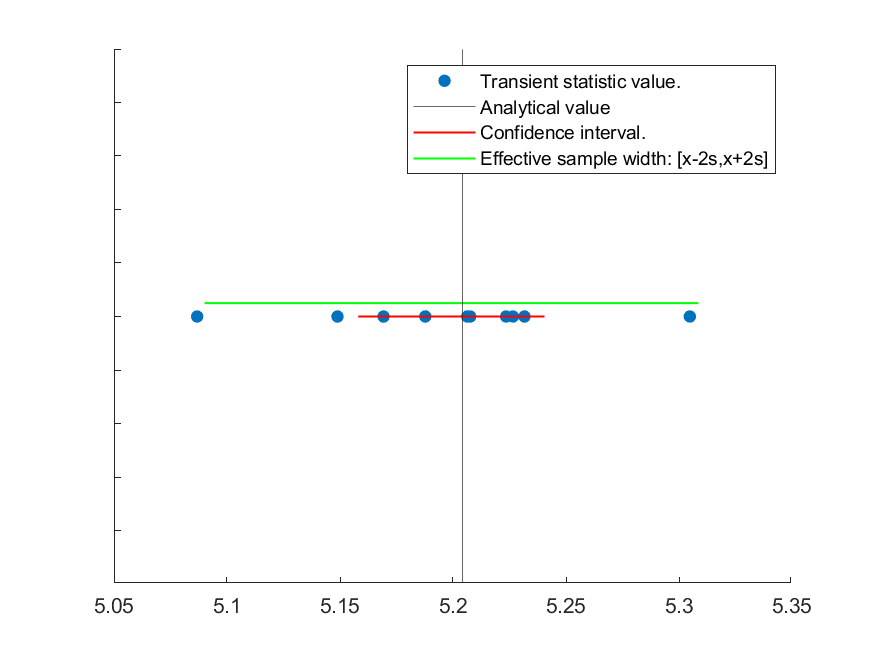
\includegraphics[width=7cm]{./GraphicsAlg1/EnsembleStatisticsCloudlet_Class1JobsNumber.png} }}%
    \subfloat{{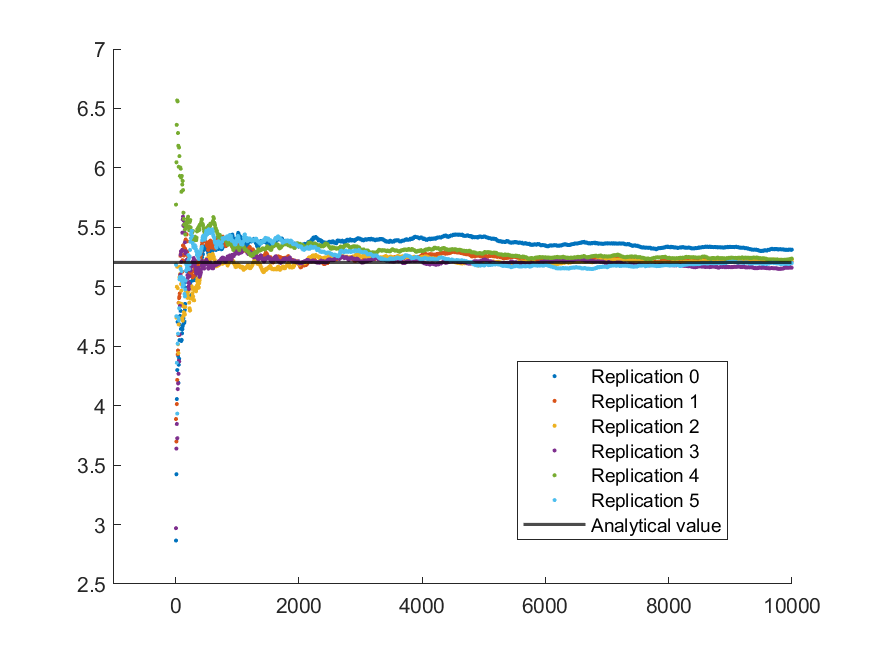
\includegraphics[width=7cm]{./GraphicsAlg1/ScatterPlotCloudlet_Class1JobsNumber.png} }}%
  
    \subfloat{{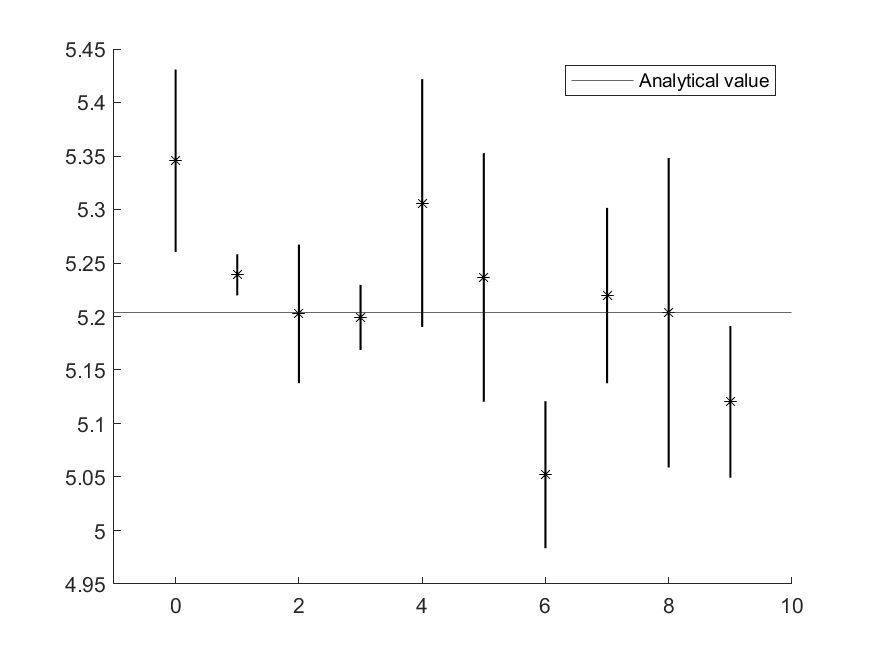
\includegraphics[width=7cm]{./GraphicsAlg1/BatchMeansCloudlet_Class1JobsNumber.png} }}%
    \subfloat{{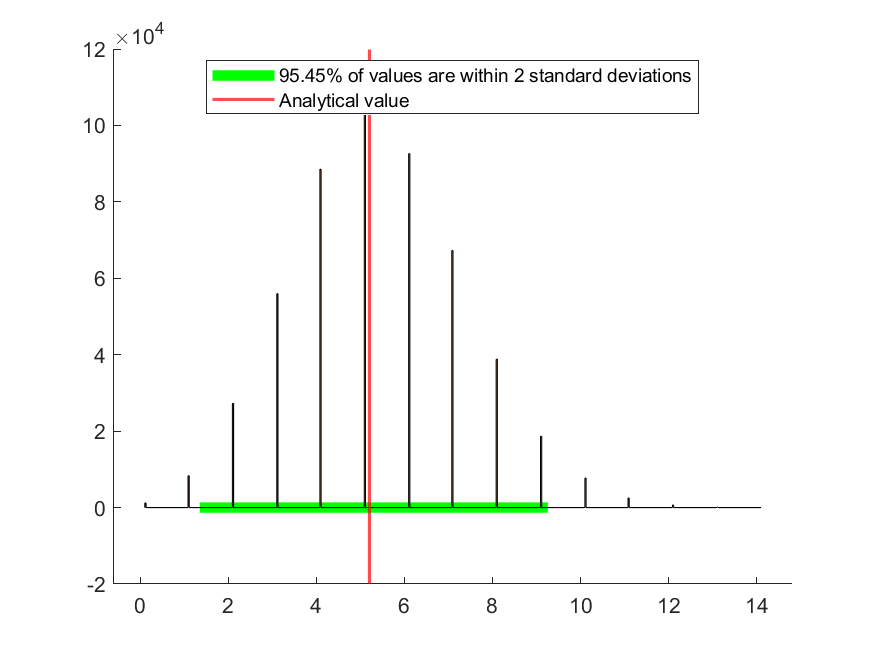
\includegraphics[width=7cm]{./GraphicsAlg1/HistogramsCloudlet_Class1JobsNumber.png} }}%
    \caption{Cloudlet}%
\end{figure}

\begin{figure}[h!]
    \centering
    \subfloat{{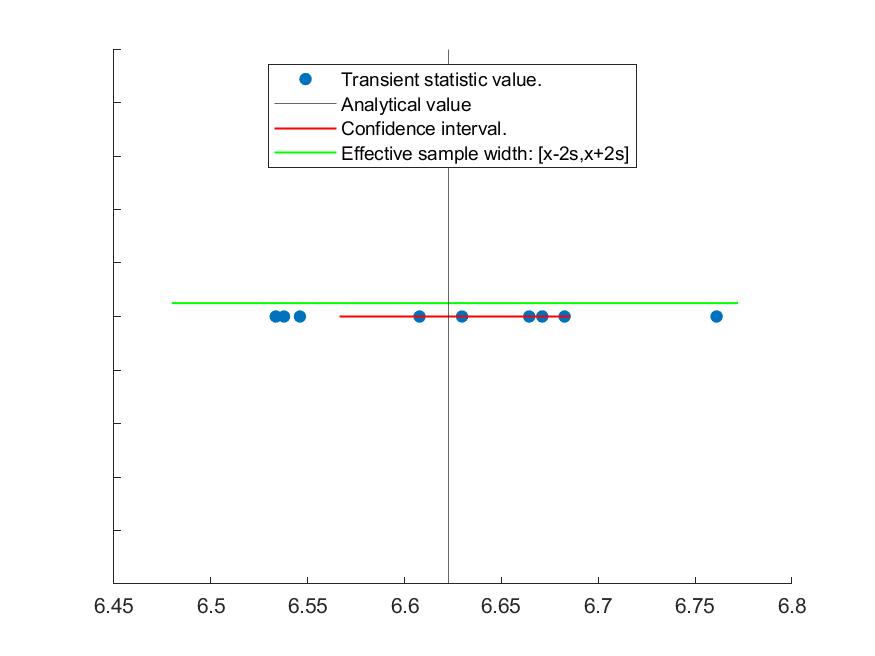
\includegraphics[width=7cm]{./GraphicsAlg1/EnsembleStatisticsCloud_Class1JobsNumber.png} }}%
    \subfloat{{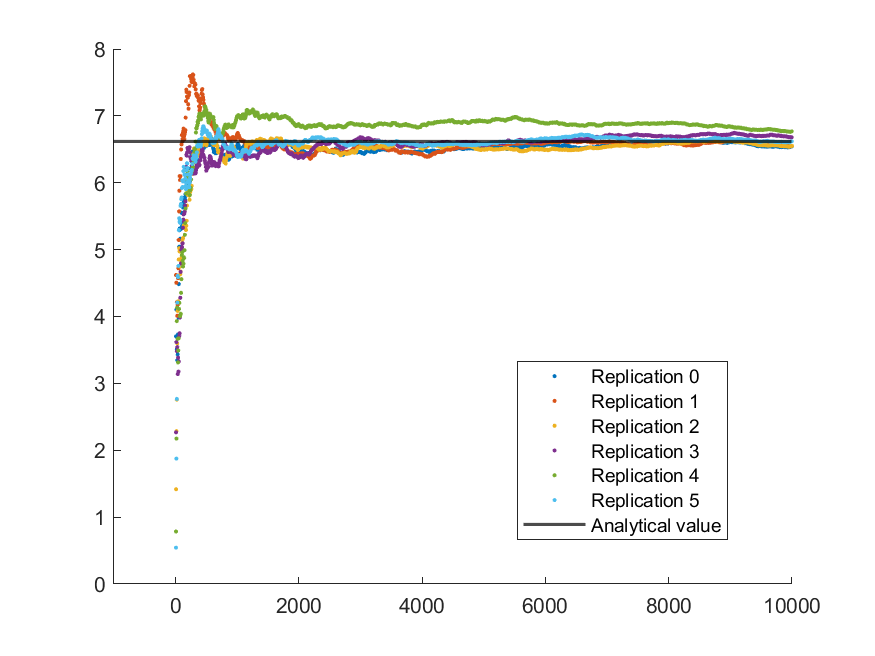
\includegraphics[width=7cm]{./GraphicsAlg1/ScatterPlotCloud_Class1JobsNumber.png} }}%
  
    \subfloat{{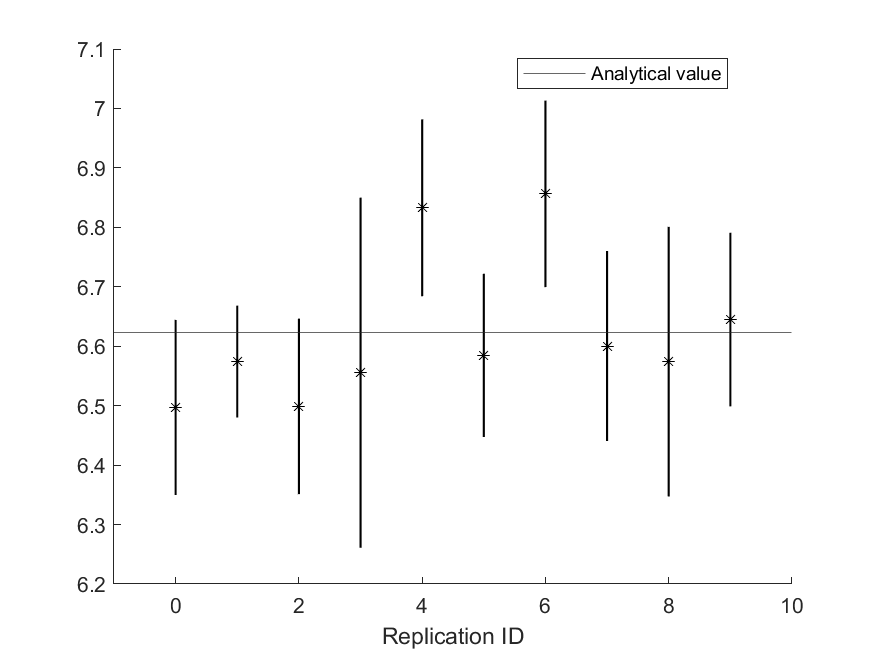
\includegraphics[width=7cm]{./GraphicsAlg1/BatchMeansCloud_Class1JobsNumber.png} }}%
    \subfloat{{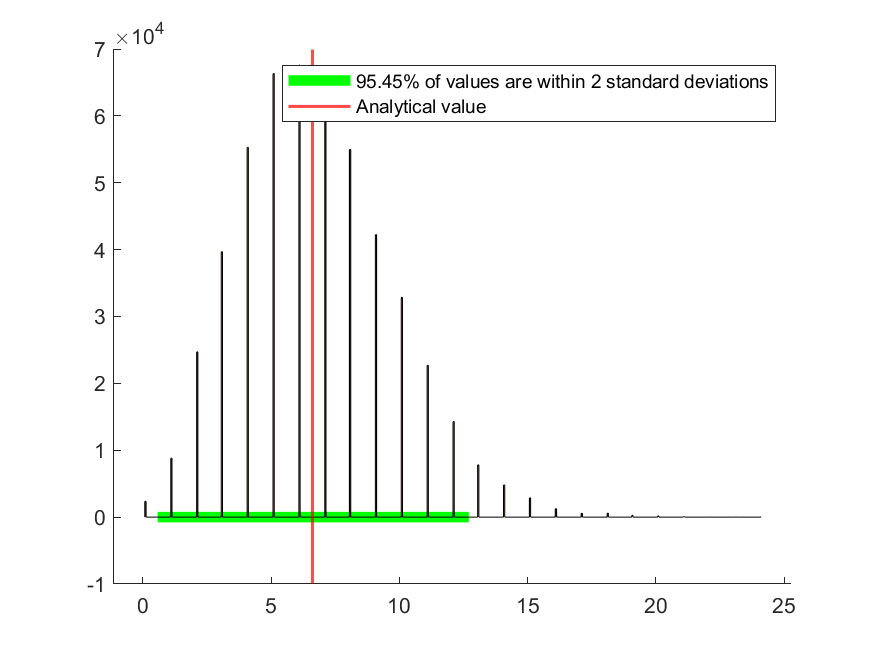
\includegraphics[width=7cm]{./GraphicsAlg1/HistogramsCloud_Class1JobsNumber.png} }}%
    \caption{Cloud}%
\end{figure}

\begin{figure}[h!]
    \centering
    \subfloat{{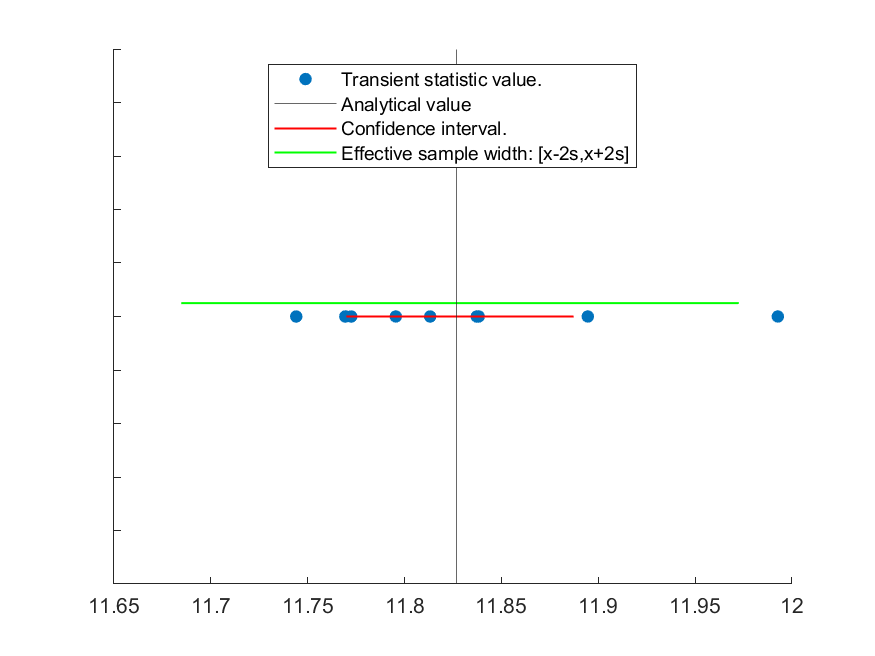
\includegraphics[width=7cm]{./GraphicsAlg1/EnsembleStatisticsGlobalNetwork_Class1JobsNumber.png} }}%
    \subfloat{{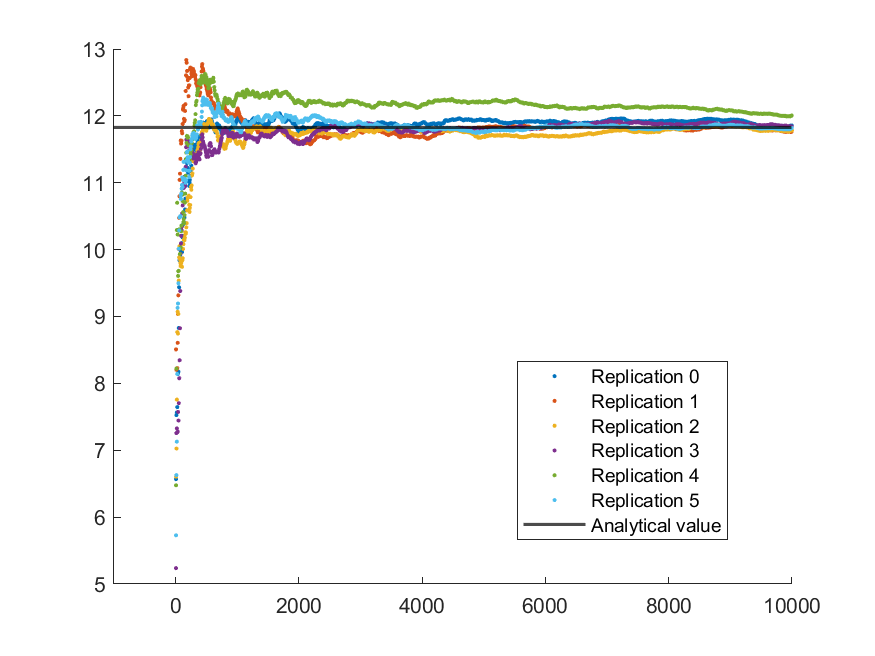
\includegraphics[width=7cm]{./GraphicsAlg1/ScatterPlotGlobalNetwork_Class1JobsNumber.png} }}%
  
    \subfloat{{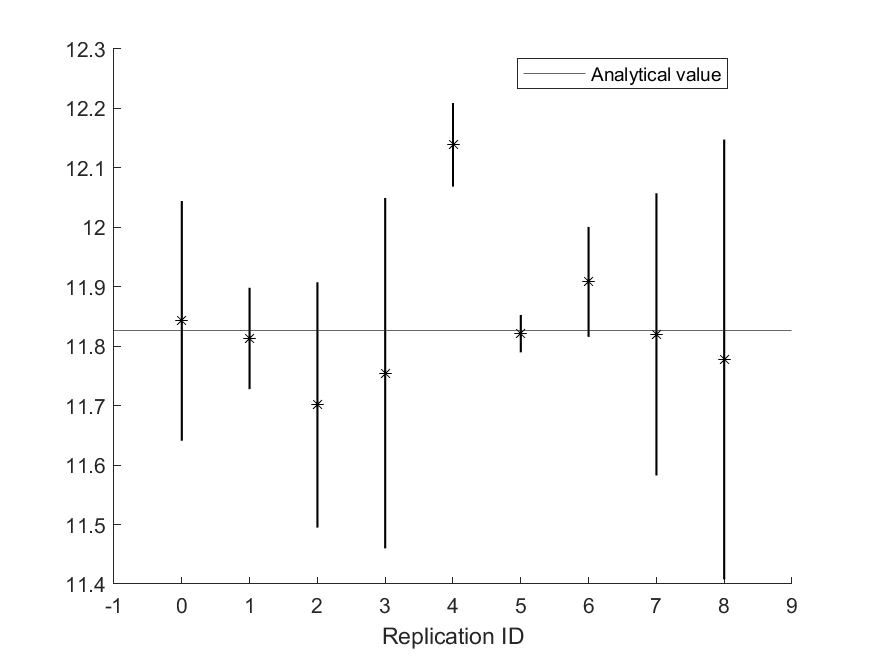
\includegraphics[width=7cm]{./GraphicsAlg1/BatchMeansGlobalNetwork_Class1JobsNumber.png} }}%
    \subfloat{{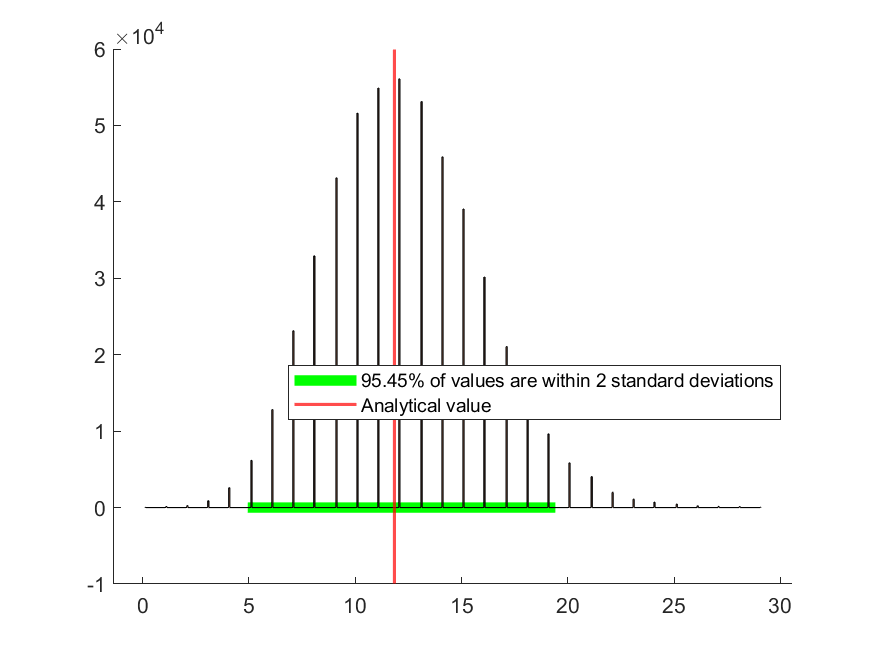
\includegraphics[width=7cm]{./GraphicsAlg1/HistogramsGlobalNetwork_Class1JobsNumber.png} }}%
    \caption{Global}%
\end{figure}

% ------------------------------------------------------------------------------------------------------------ %
% JOB 2 POPULATION
% ------------------------------------------------------------------------------------------------------------ %

\clearpage
\newpage
\subsubsection{Time-Average Class 2 Job Population}

\begin{figure}[h!]
    \centering
    \subfloat{{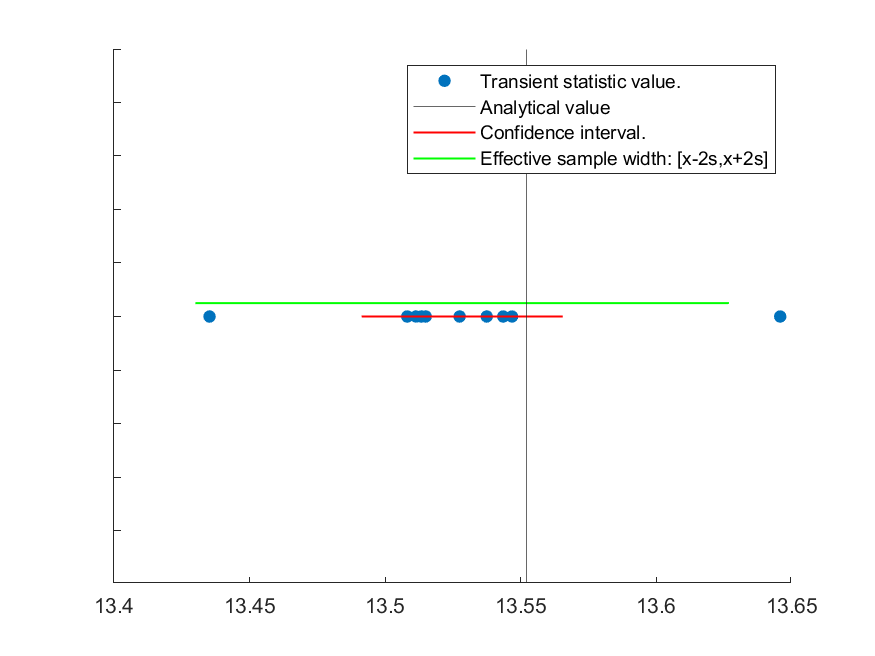
\includegraphics[width=7cm]{./GraphicsAlg1/EnsembleStatisticsCloudlet_Class2JobsNumber.png} }}%
    \subfloat{{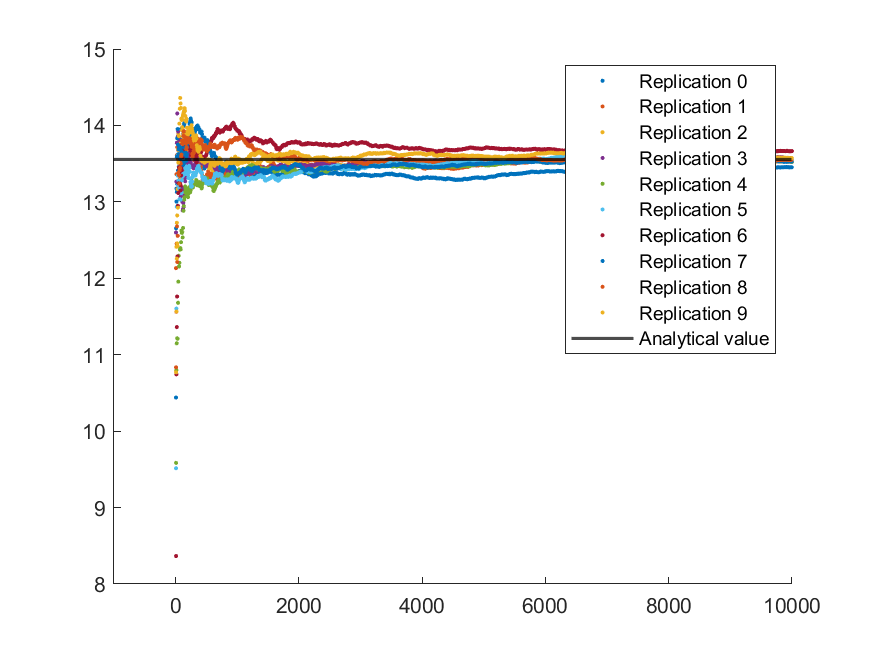
\includegraphics[width=7cm]{./GraphicsAlg1/ScatterPlotCloudlet_Class2JobsNumber.png} }}%
  
    \subfloat{{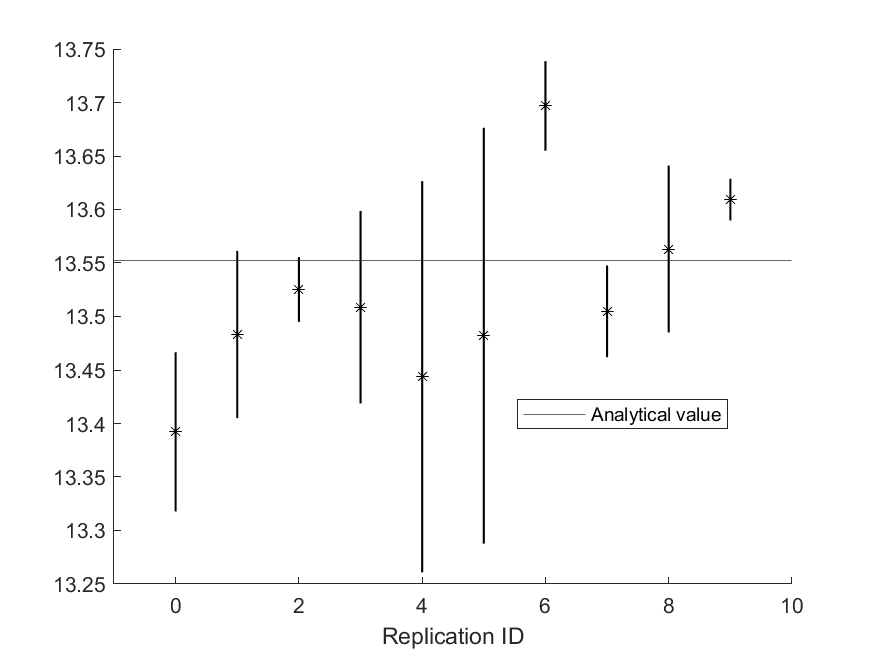
\includegraphics[width=7cm]{./GraphicsAlg1/BatchMeansCloudlet_Class2JobsNumber.png} }}%
    \subfloat{{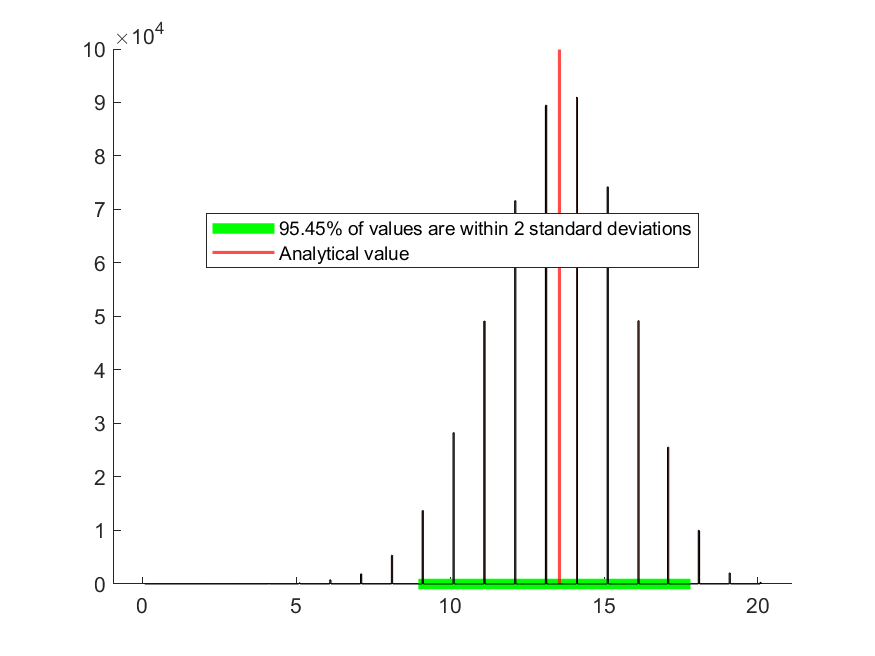
\includegraphics[width=7cm]{./GraphicsAlg1/HistogramsCloudlet_Class2JobsNumber.png} }}%
    \caption{Cloudlet}%
\end{figure}

\begin{figure}[h!]
    \centering
    \subfloat{{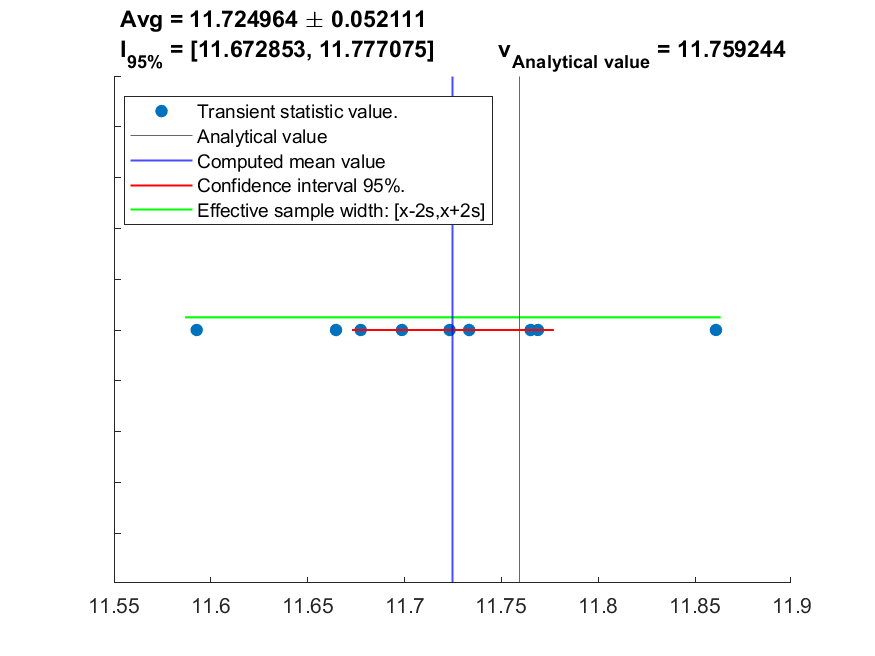
\includegraphics[width=7cm]{./GraphicsAlg1/EnsembleStatisticsCloud_Class2JobsNumber.png} }}%
    \subfloat{{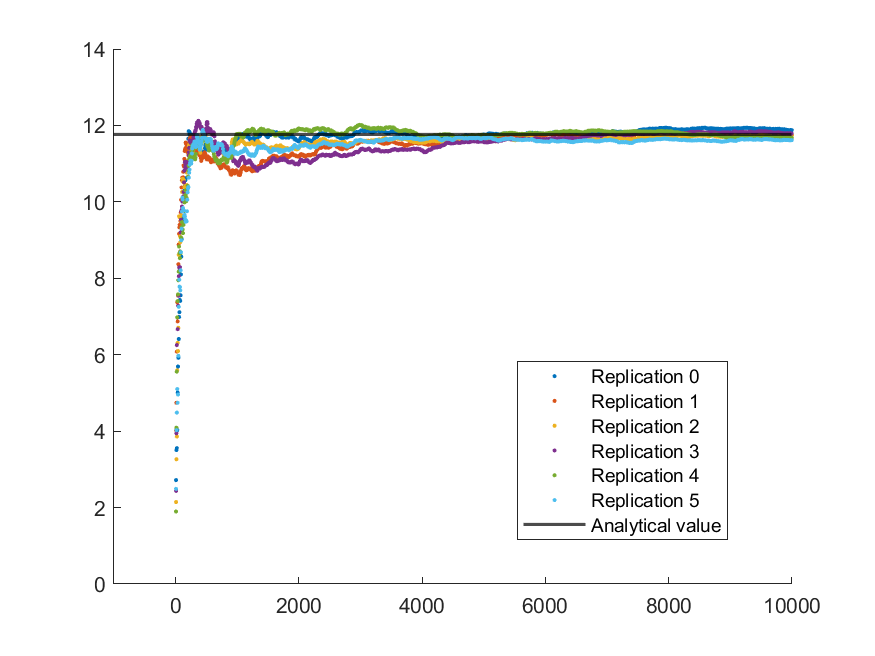
\includegraphics[width=7cm]{./GraphicsAlg1/ScatterPlotCloud_Class2JobsNumber.png} }}%
  
    \subfloat{{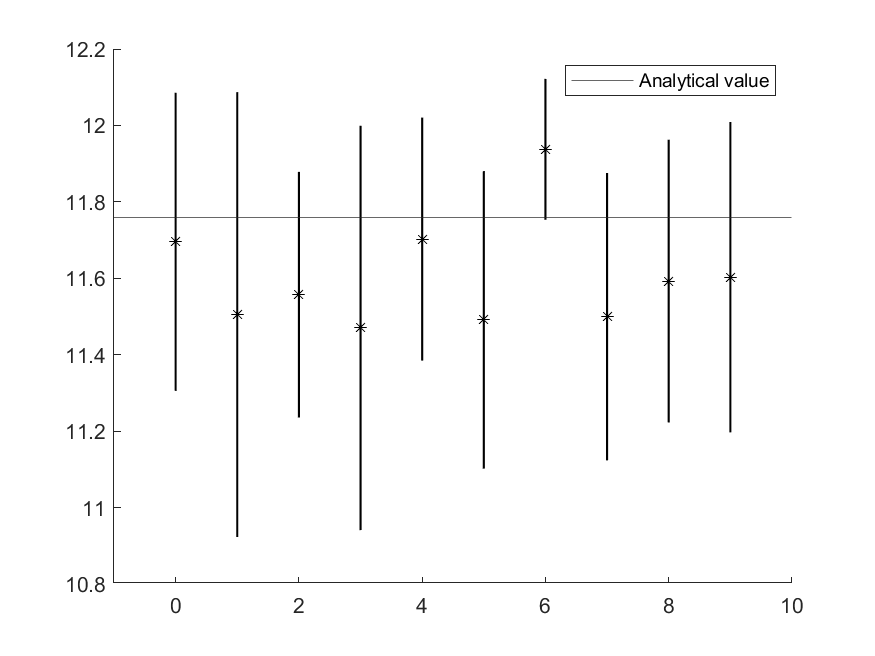
\includegraphics[width=7cm]{./GraphicsAlg1/BatchMeansCloud_Class2JobsNumber.png} }}%
    \subfloat{{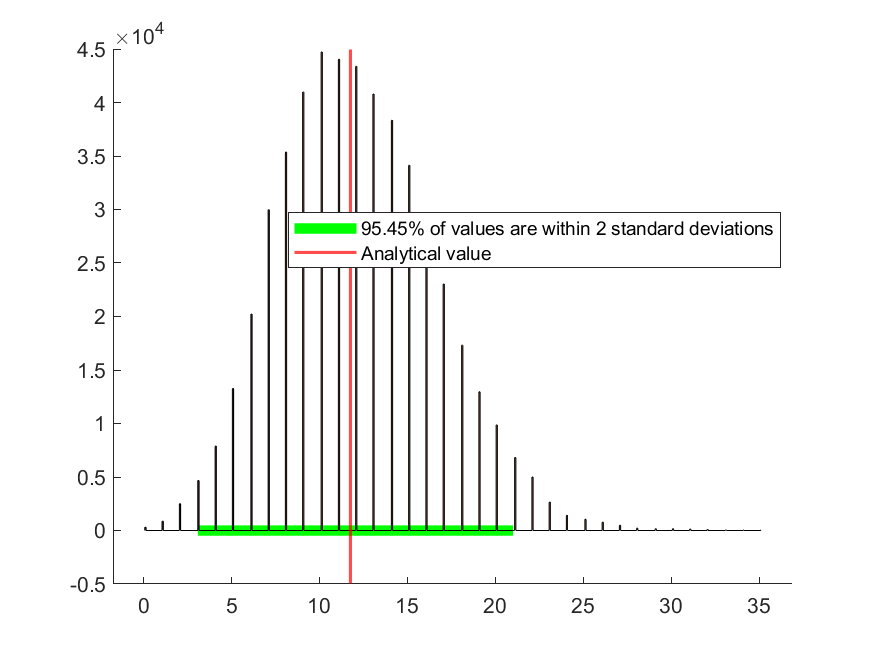
\includegraphics[width=7cm]{./GraphicsAlg1/HistogramsCloud_Class2JobsNumber.png} }}%
    \caption{Cloud}%
\end{figure}

\begin{figure}[h!]
    \centering
    \subfloat{{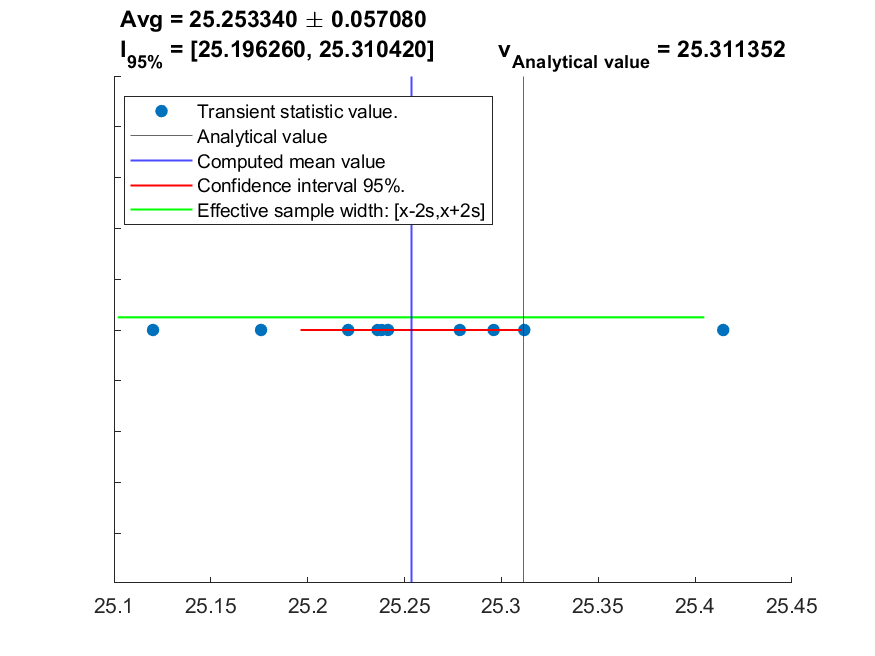
\includegraphics[width=7cm]{./GraphicsAlg1/EnsembleStatisticsGlobalNetwork_Class2JobsNumber.png} }}%
    \subfloat{{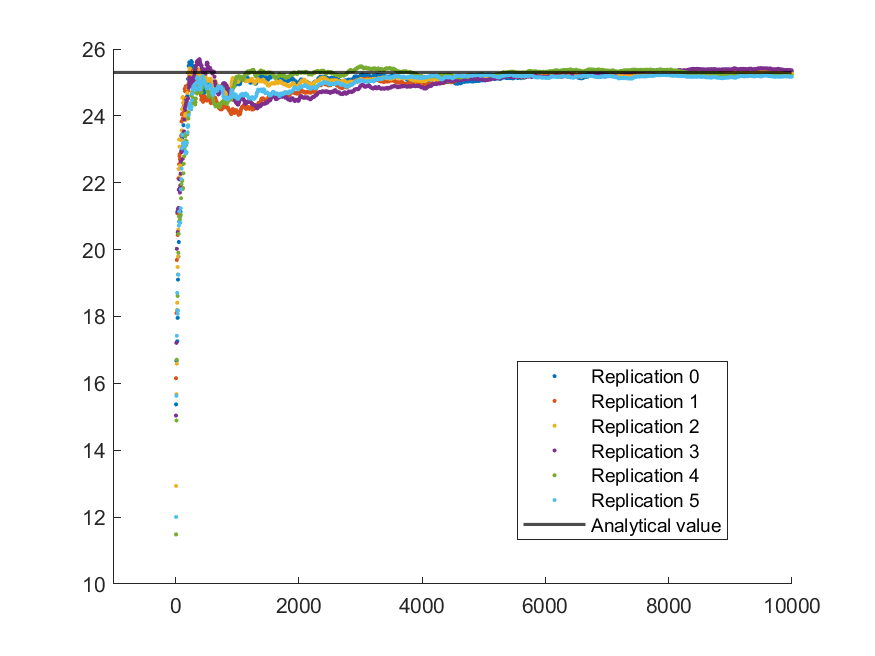
\includegraphics[width=7cm]{./GraphicsAlg1/ScatterPlotGlobalNetwork_Class2JobsNumber.png} }}%
  
    \subfloat{{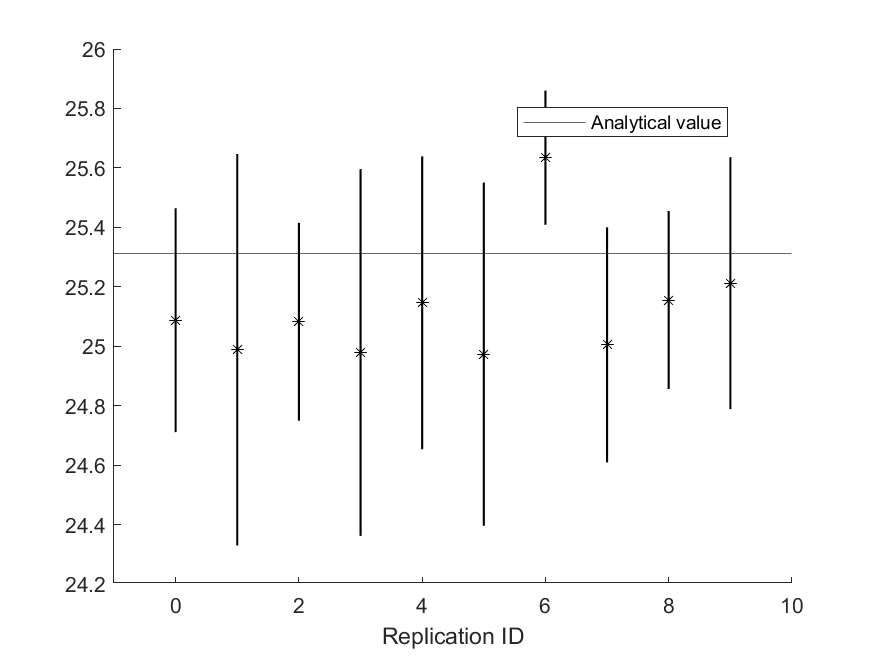
\includegraphics[width=7cm]{./GraphicsAlg1/BatchMeansGlobalNetwork_Class2JobsNumber.png} }}%
    \subfloat{{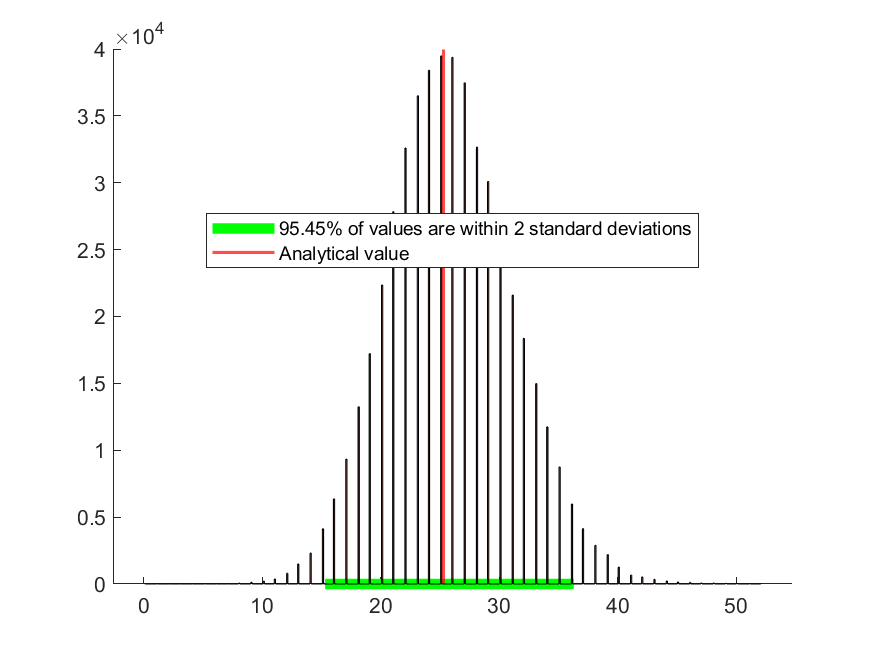
\includegraphics[width=7cm]{./GraphicsAlg1/HistogramsGlobalNetwork_Class2JobsNumber.png} }}%
    \caption{Global}%
\end{figure}



% ------------------------------------------------------------------------------------------------------------ %
% JOB POPULATION
% ------------------------------------------------------------------------------------------------------------ %

\clearpage
\newpage
\subsubsection{Time-Average Job Population}

\begin{figure}[h!]
    \centering
    \subfloat{{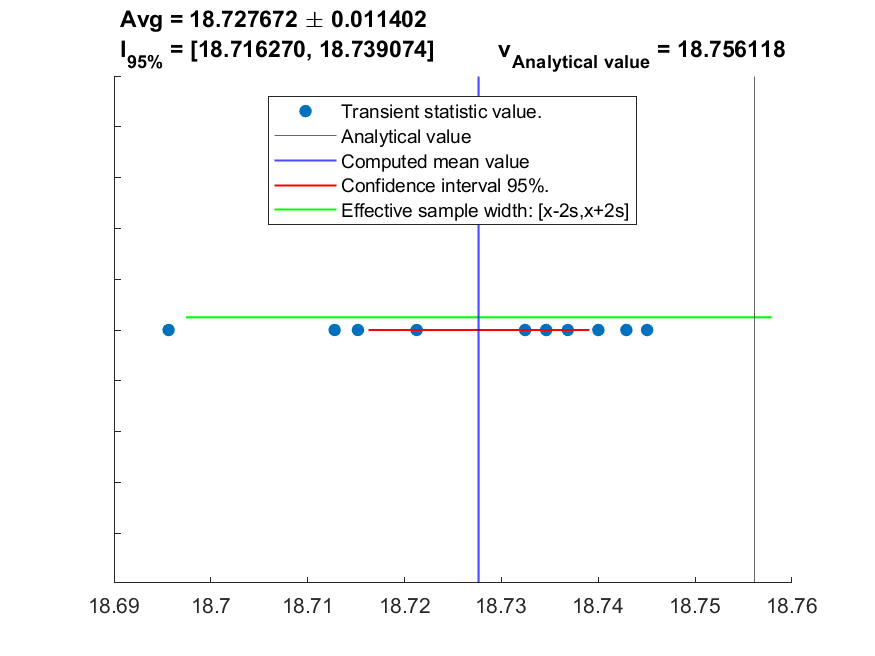
\includegraphics[width=7cm]{./GraphicsAlg1/EnsembleStatisticsCloudlet_JobsNumber.png} }}%
    \subfloat{{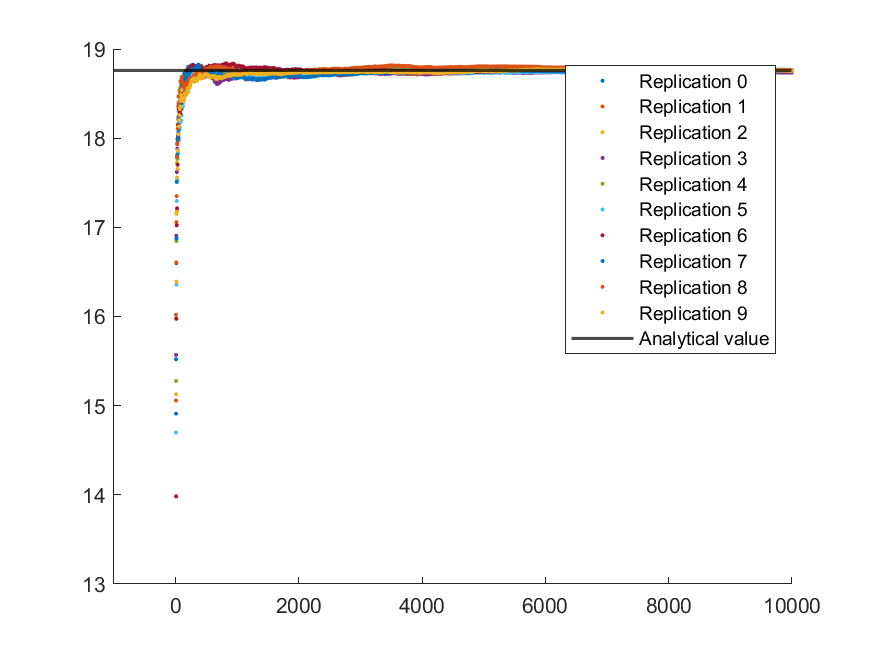
\includegraphics[width=7cm]{./GraphicsAlg1/ScatterPlotCloudlet_JobsNumber.png} }}%
    
    \subfloat{{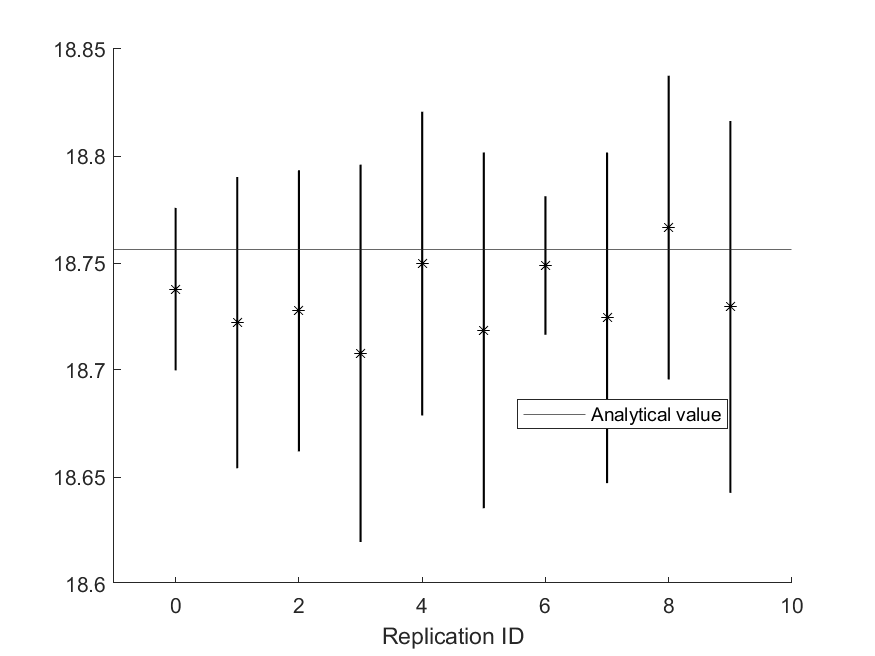
\includegraphics[width=7cm]{./GraphicsAlg1/BatchMeansCloudlet_JobsNumber.png} }}%
    \subfloat{{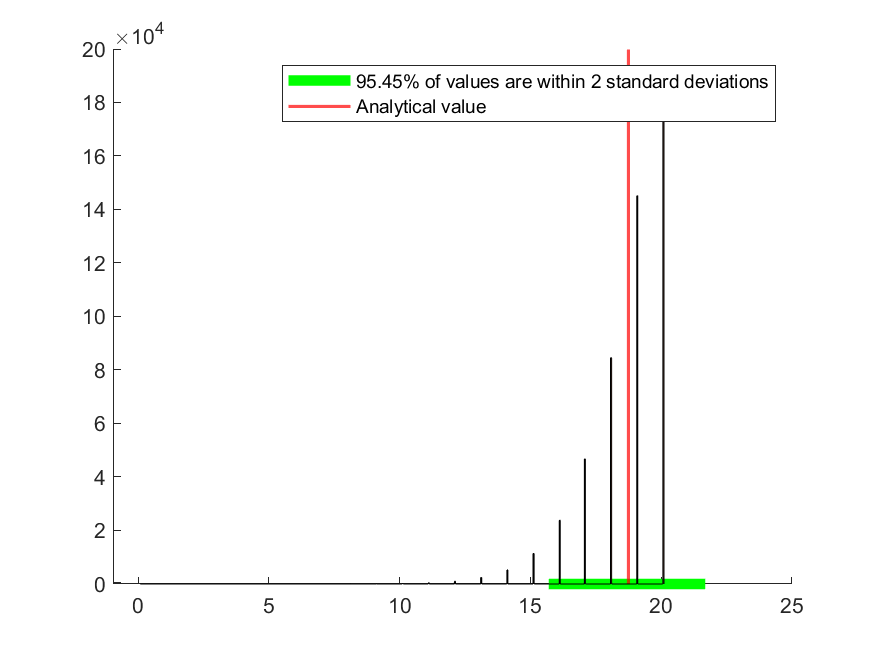
\includegraphics[width=7cm]{./GraphicsAlg1/HistogramsCloudlet_JobsNumber.png} }}%
    \caption{Cloudlet}%
\end{figure}

\begin{figure}[h!]
    \centering
    \subfloat{{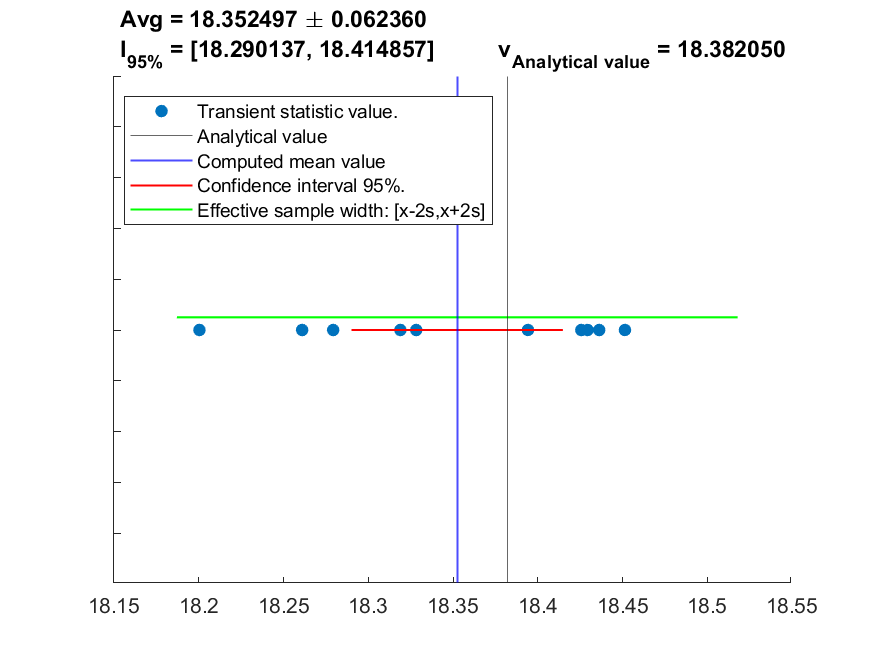
\includegraphics[width=7cm]{./GraphicsAlg1/EnsembleStatisticsCloud_JobsNumber.png} }}%
    \subfloat{{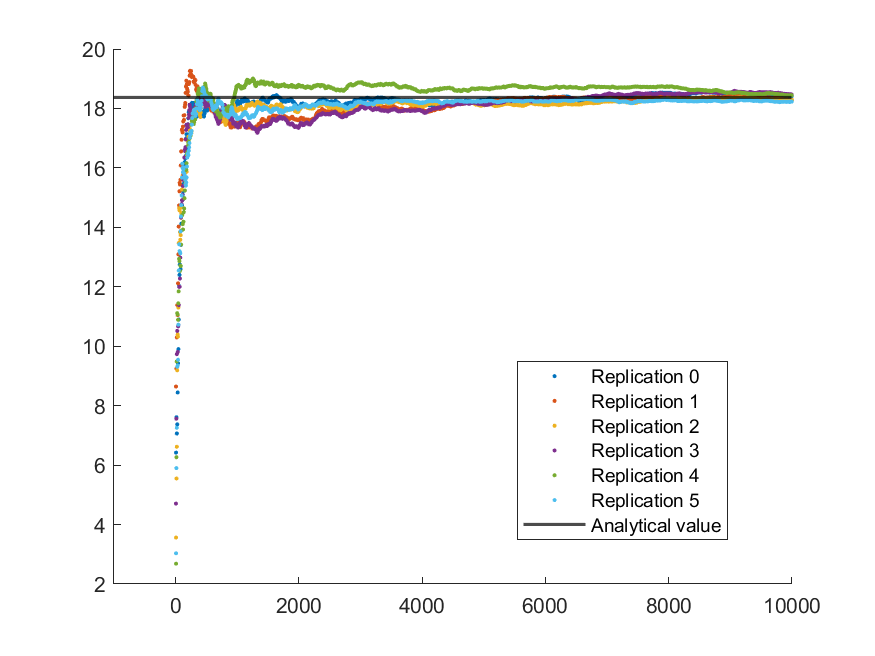
\includegraphics[width=7cm]{./GraphicsAlg1/ScatterPlotCloud_JobsNumber.png} }}%
  
    \subfloat{{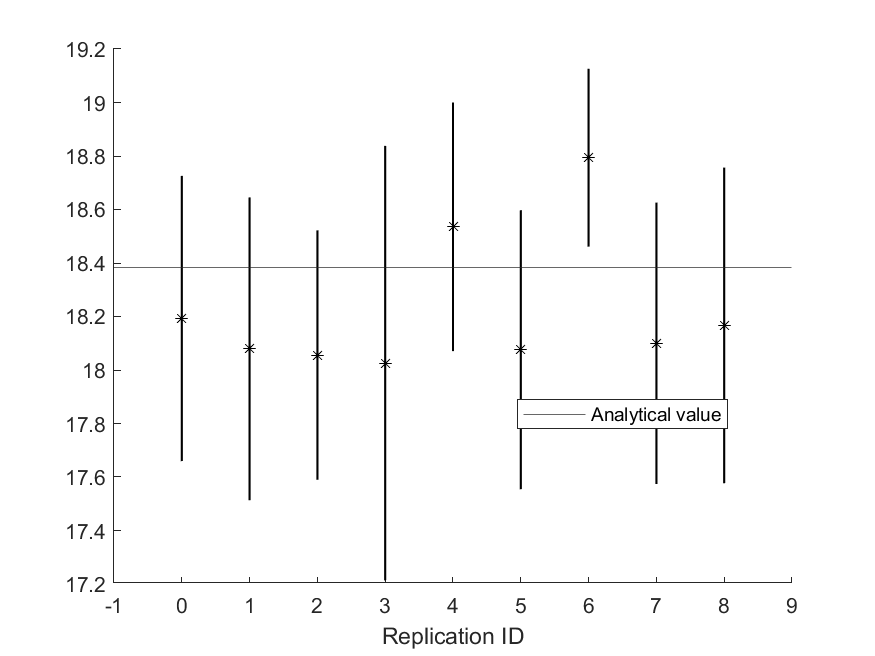
\includegraphics[width=7cm]{./GraphicsAlg1/BatchMeansCloud_JobsNumber.png} }}%
    \subfloat{{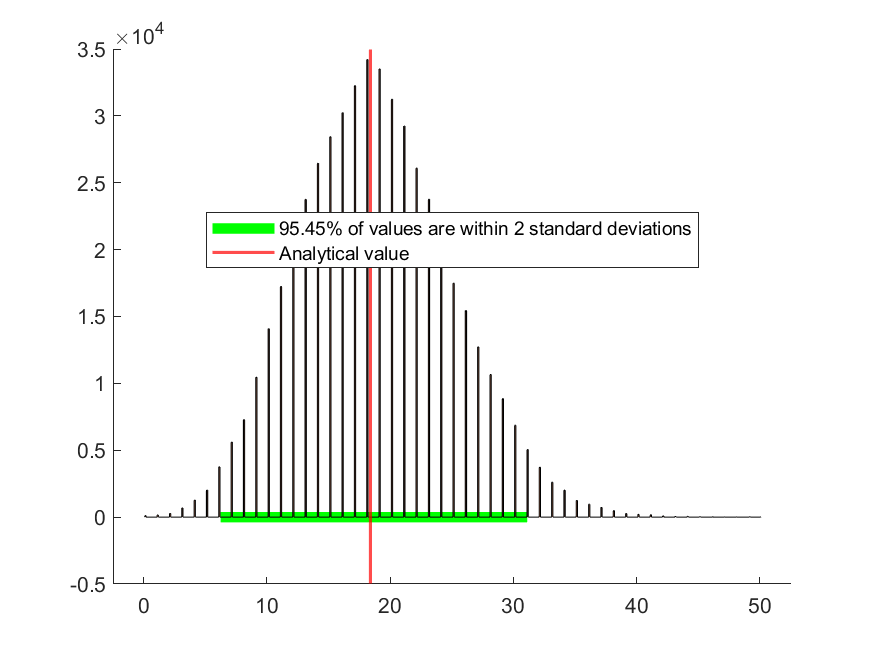
\includegraphics[width=7cm]{./GraphicsAlg1/HistogramsCloud_JobsNumber.png} }}%
    \caption{Cloud}%
\end{figure}

\begin{figure}[h!]
    \centering
    \subfloat{{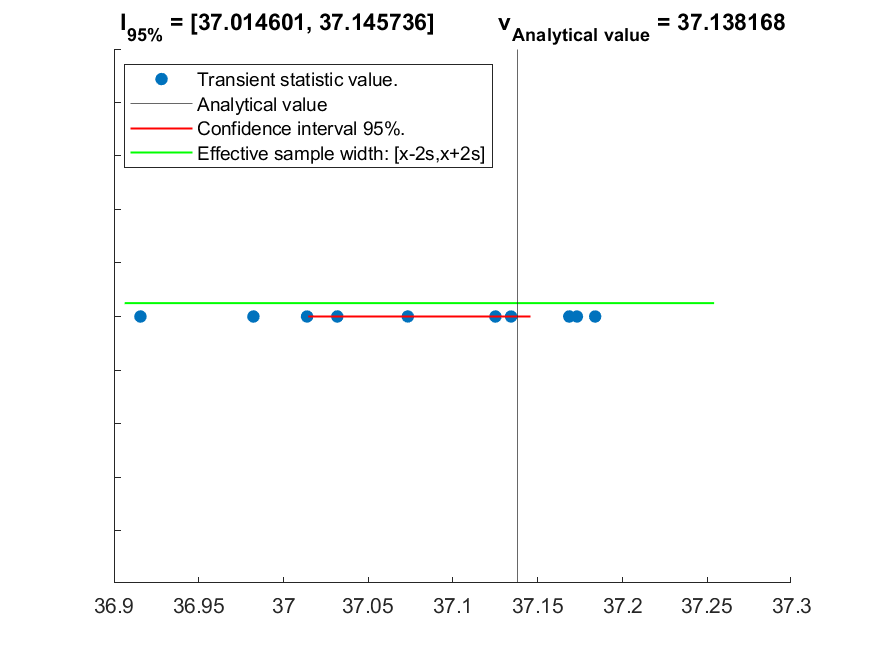
\includegraphics[width=7cm]{./GraphicsAlg1/EnsembleStatisticsGlobalNetwork_JobsNumber.png} }}%
    \subfloat{{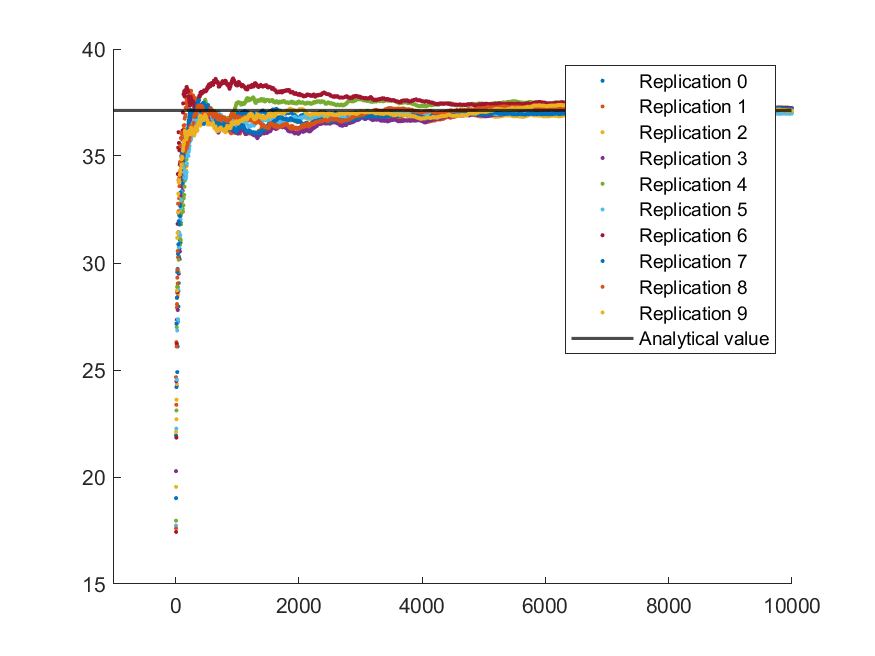
\includegraphics[width=7cm]{./GraphicsAlg1/ScatterPlotGlobalNetwork_JobsNumber.png} }}%
    
    \subfloat{{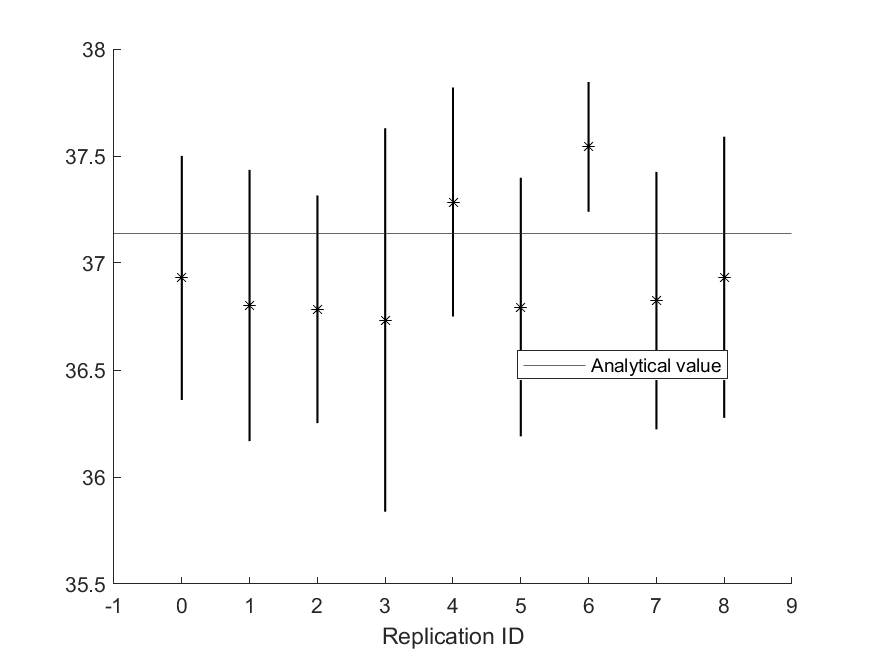
\includegraphics[width=7cm]{./GraphicsAlg1/BatchMeansGlobalNetwork_JobsNumber.png} }}%
    \subfloat{{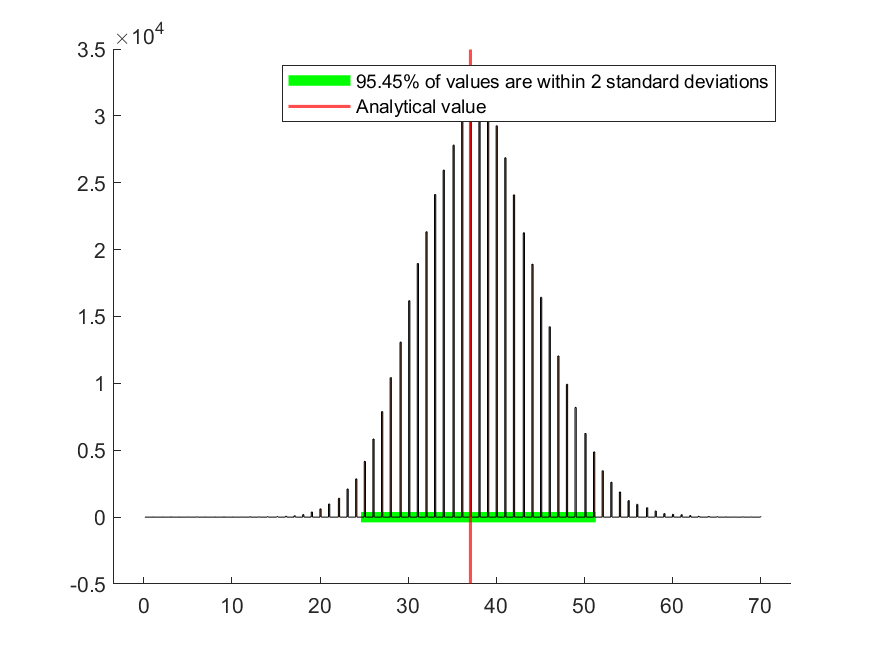
\includegraphics[width=7cm]{./GraphicsAlg1/HistogramsGlobalNetwork_JobsNumber.png} }}%
    \caption{Global}%
\end{figure}

% ------------------------------------------------------------------------------------------------------------ %
% Class1JobsServiceTime
% ------------------------------------------------------------------------------------------------------------ %

\newpage
\newgeometry{top=10mm, left=8mm, right=8mm}
\subsubsection{Time-Average Class 1 Job Service/Response Time}

\begin{figure}[h!]
    \centering
    \subfloat{{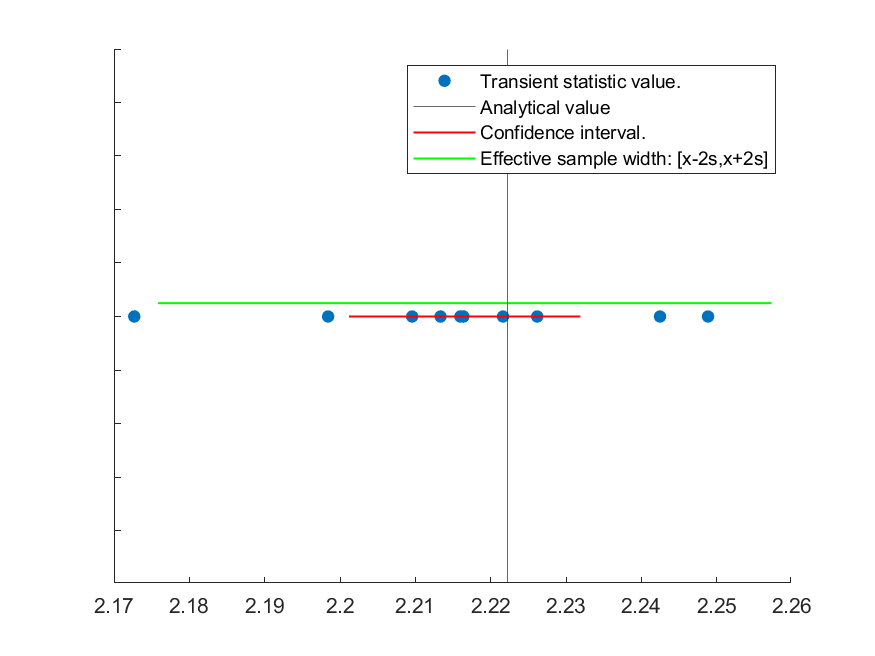
\includegraphics[width=6.5cm]{./GraphicsAlg1/EnsembleStatisticsCloudlet_Class1JobsServiceTime.png} }}%
    \subfloat{{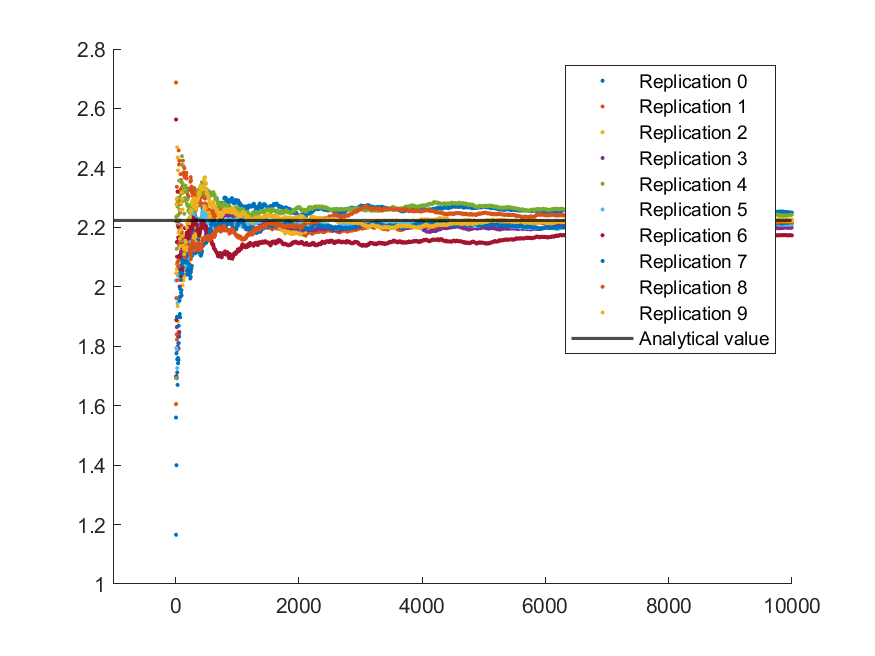
\includegraphics[width=6.5cm]{./GraphicsAlg1/ScatterPlotCloudlet_Class1JobsServiceTime.png} }}%  
    \subfloat{{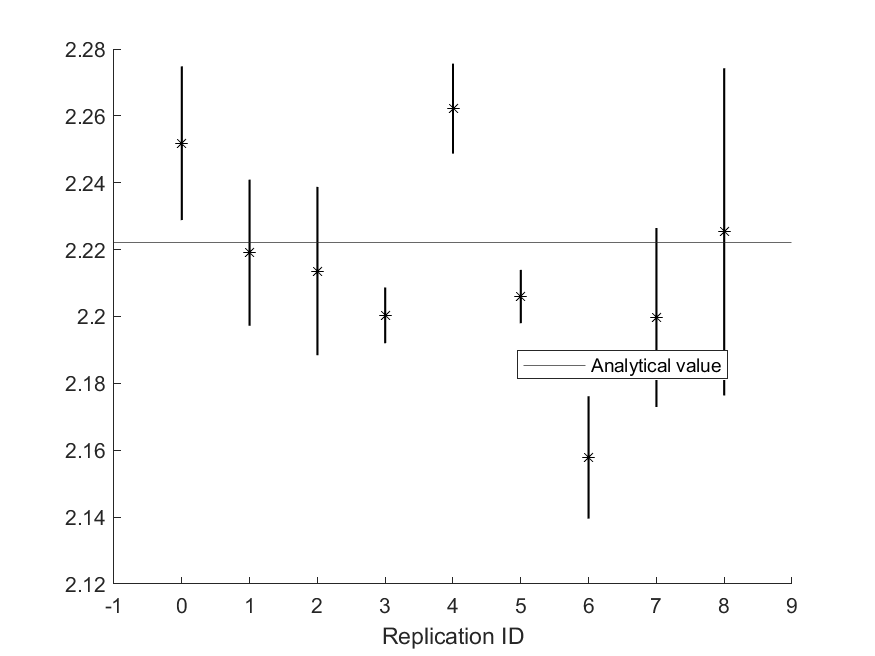
\includegraphics[width=6.5cm]{./GraphicsAlg1/BatchMeansCloudlet_Class1JobsServiceTime.png} }}%
    \caption{Cloudlet}%
    \label{fig:example}
\end{figure}

\begin{figure}[h!]
    \centering
    \subfloat{{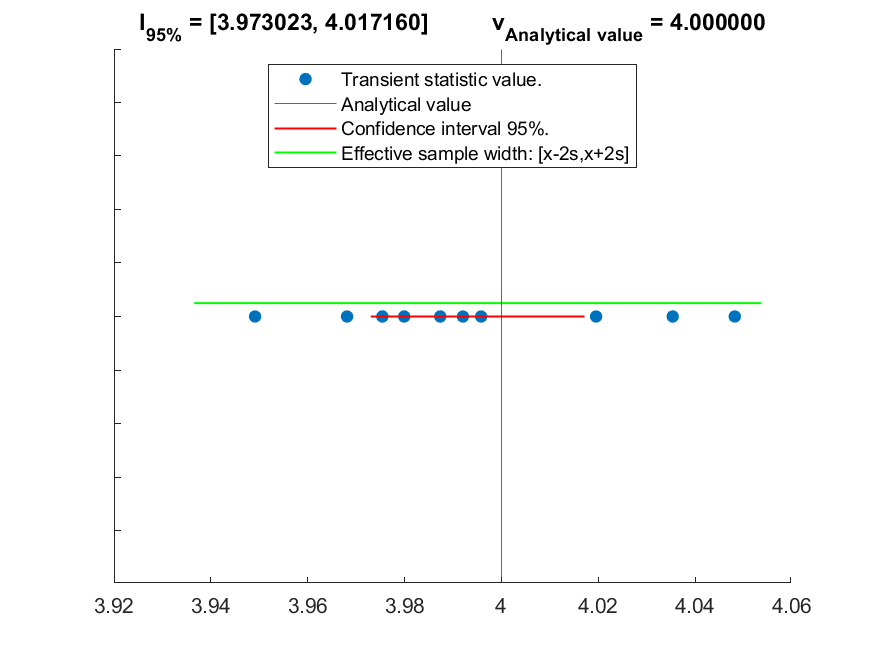
\includegraphics[width=6.5cm]{./GraphicsAlg1/EnsembleStatisticsCloud_Class1JobsServiceTime.png} }}%
    \subfloat{{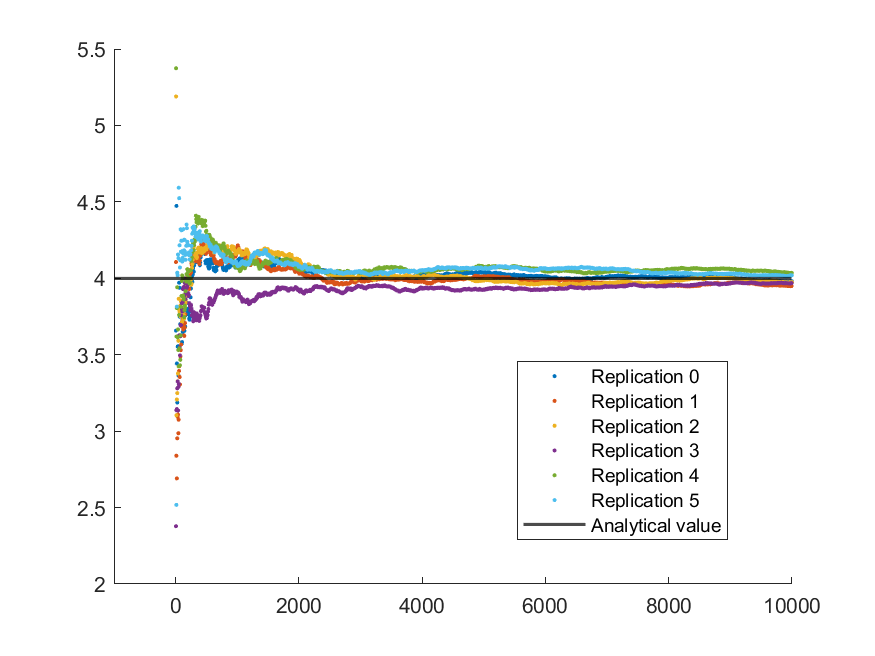
\includegraphics[width=6.5cm]{./GraphicsAlg1/ScatterPlotCloud_Class1JobsServiceTime.png} }}%  
    \subfloat{{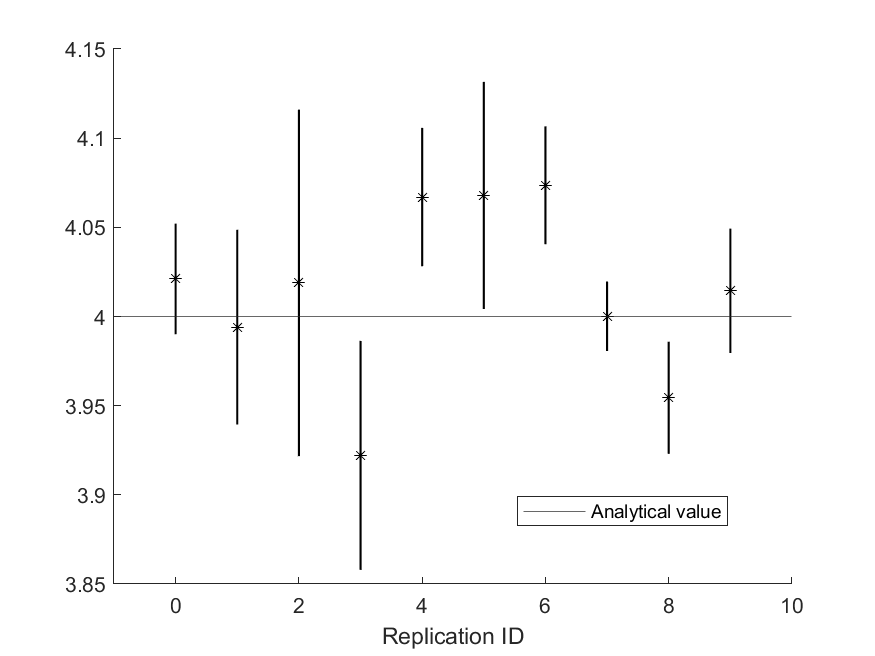
\includegraphics[width=6.5cm]{./GraphicsAlg1/BatchMeansCloud_Class1JobsServiceTime.png} }}%
    \caption{Cloud}%
    \label{fig:example}
\end{figure}

\begin{figure}[h!]
    \centering
    \subfloat{{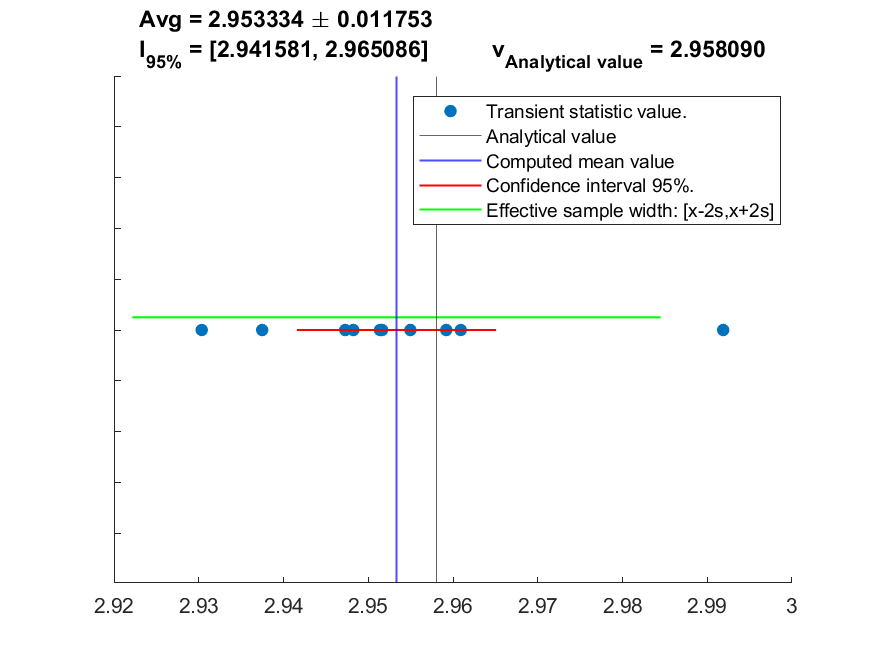
\includegraphics[width=6.5cm]{./GraphicsAlg1/EnsembleStatisticsGlobalNetwork_Class1JobsServiceTime.png} }}%
    \subfloat{{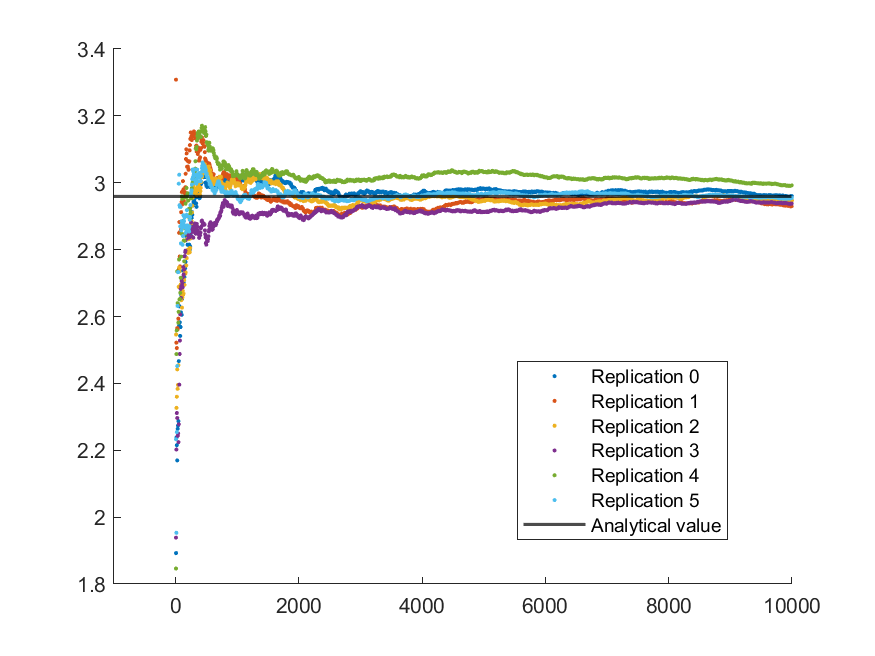
\includegraphics[width=6.5cm]{./GraphicsAlg1/ScatterPlotGlobalNetwork_Class1JobsServiceTime.png} }}%   
    \subfloat{{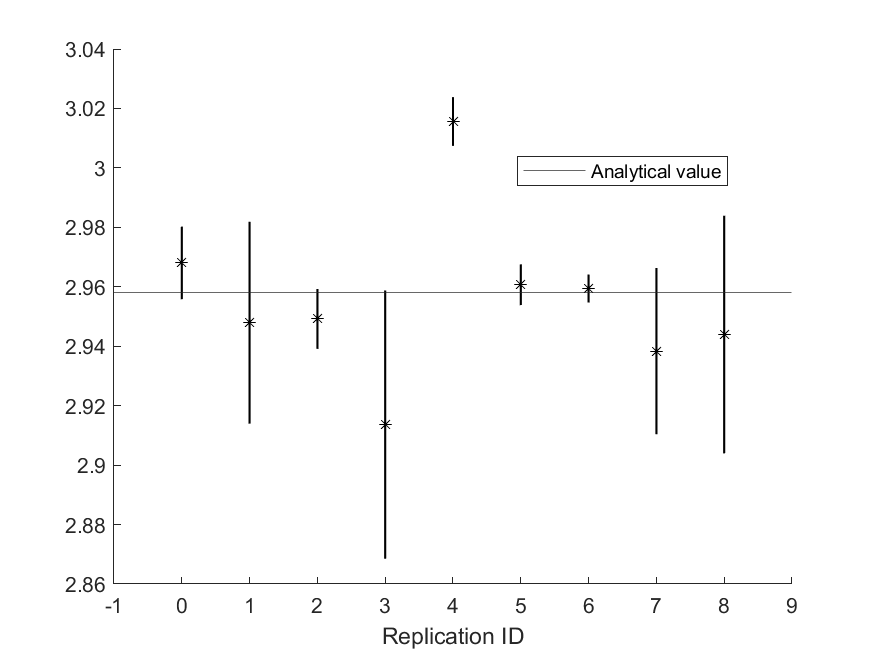
\includegraphics[width=6.5cm]{./GraphicsAlg1/BatchMeansGlobalNetwork_Class1JobsServiceTime.png} }}%
   
    \caption{Global}%
    \label{fig:example}
\end{figure}
\restoregeometry 

% ------------------------------------------------------------------------------------------------------------ %
% Class2JobsServiceTime
% ------------------------------------------------------------------------------------------------------------ %

\newpage
\newgeometry{top=10mm, left=8mm, right=8mm}
\subsubsection{Time-Average Class 2 Job Service/Response Time}

\begin{figure}[h!]
    \centering
    \subfloat{{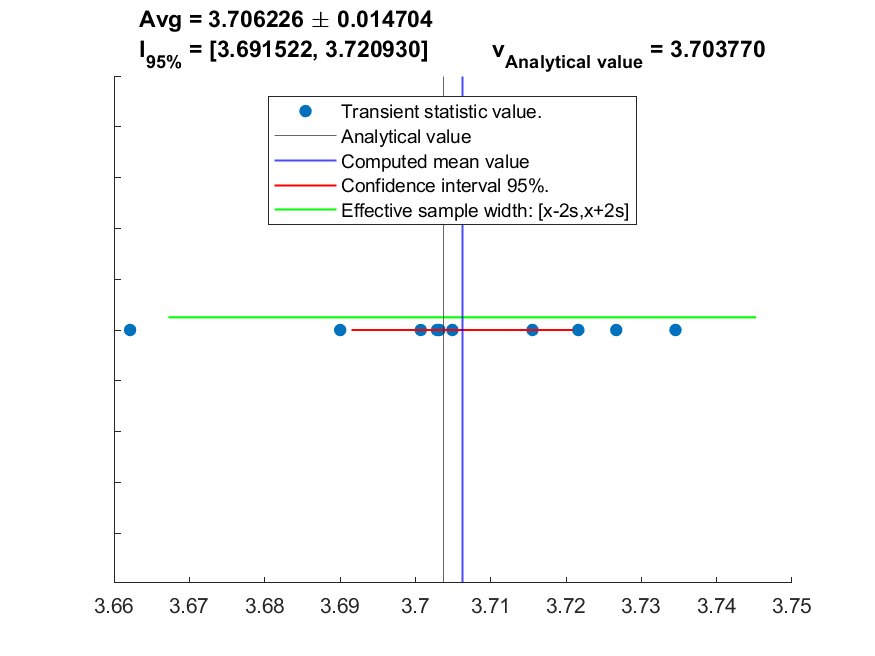
\includegraphics[width=6.5cm]{./GraphicsAlg1/EnsembleStatisticsCloudlet_Class2JobsServiceTime.png} }}%
    \subfloat{{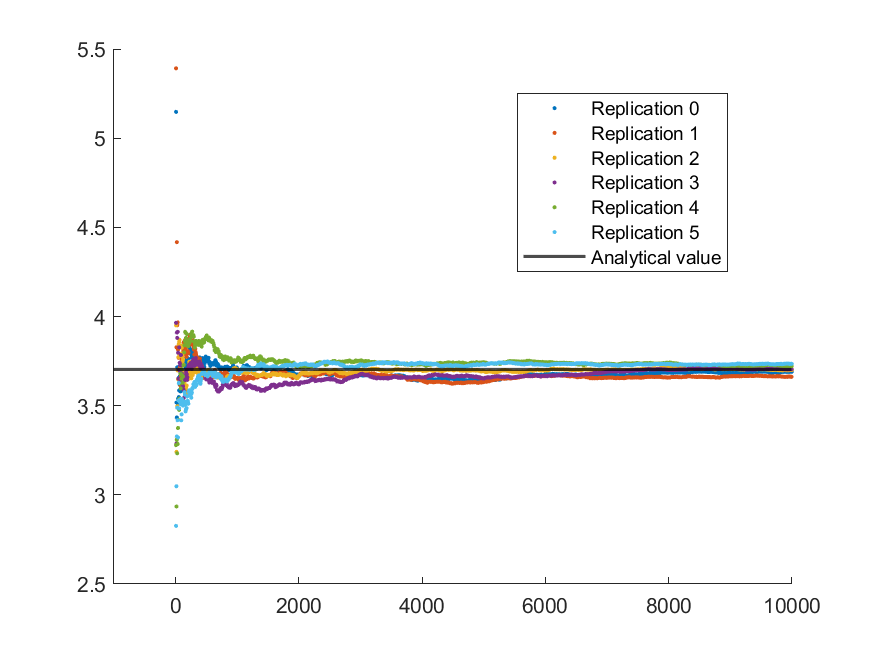
\includegraphics[width=6.5cm]{./GraphicsAlg1/ScatterPlotCloudlet_Class2JobsServiceTime.png} }}%  
    \subfloat{{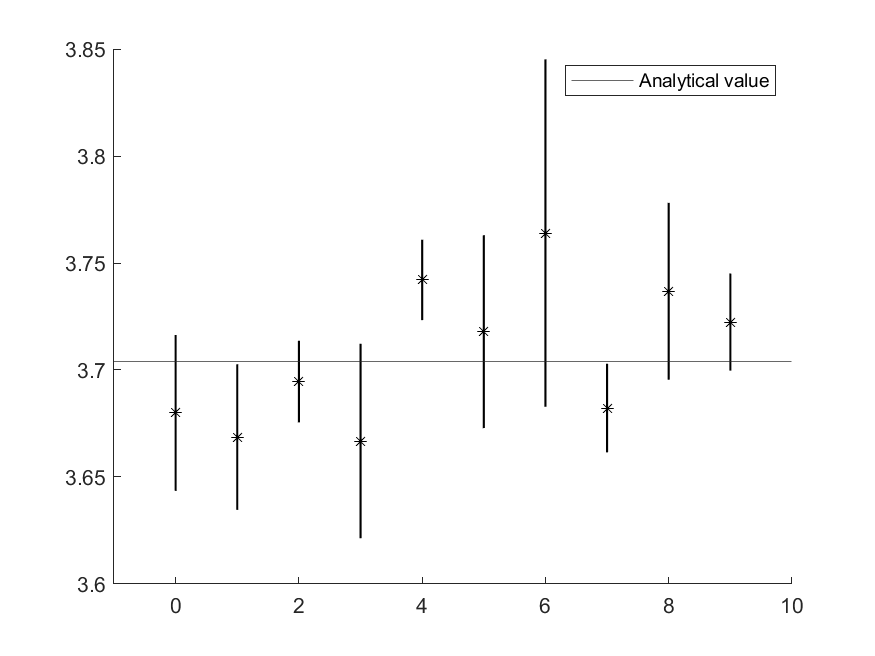
\includegraphics[width=6.5cm]{./GraphicsAlg1/BatchMeansCloudlet_Class2JobsServiceTime.png} }}%
    \caption{Cloudlet}%
    \label{fig:example}
\end{figure}

\begin{figure}[h!]
    \centering
    \subfloat{{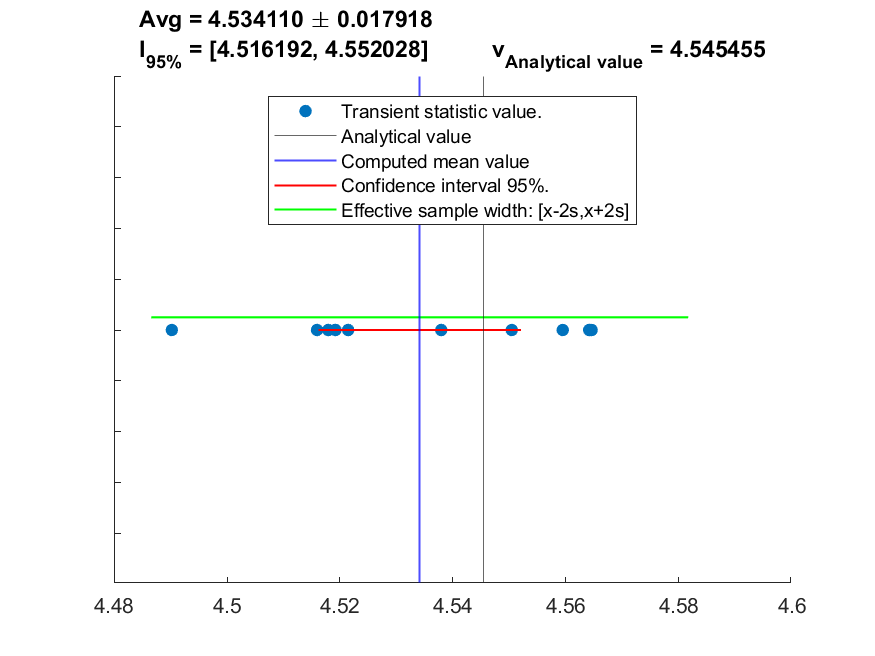
\includegraphics[width=6.5cm]{./GraphicsAlg1/EnsembleStatisticsCloud_Class2JobsServiceTime.png} }}%
    \subfloat{{\includegraphics[width=6.5cm]{./GraphicsAlg1/ScatterPlotCloud_Class2JobsServiceTime.png} }}%  
    \subfloat{{\includegraphics[width=6.5cm]{./GraphicsAlg1/BatchMeansCloud_Class2JobsServiceTime.png} }}%
    \caption{Cloud}%
    \label{fig:example}
\end{figure}

\begin{figure}[h!]
    \centering
    \subfloat{{\includegraphics[width=6.5cm]{./GraphicsAlg1/EnsembleStatisticsGlobalNetwork_Class2JobsServiceTime.png} }}%
    \subfloat{{\includegraphics[width=6.5cm]{./GraphicsAlg1/ScatterPlotGlobalNetwork_Class2JobsServiceTime.png} }}%   
    \subfloat{{\includegraphics[width=6.5cm]{./GraphicsAlg1/BatchMeansGlobalNetwork_Class2JobsServiceTime.png} }}%
   
    \caption{Global}%
    \label{fig:example}
\end{figure}
\restoregeometry 

% ------------------------------------------------------------------------------------------------------------ %
% JobsServiceTime
% ------------------------------------------------------------------------------------------------------------ %

\newpage
\newgeometry{top=10mm, left=8mm, right=8mm}
\subsubsection{Time-Average Service/Response Time}

\begin{figure}[h!]
    \centering
    \subfloat{{\includegraphics[width=6.5cm]{./GraphicsAlg1/EnsembleStatisticsCloudlet_JobsServiceTime.png} }}%
    \subfloat{{\includegraphics[width=6.5cm]{./GraphicsAlg1/ScatterPlotCloudlet_JobsServiceTime.png} }}%
    \subfloat{{\includegraphics[width=6.5cm]{./GraphicsAlg1/BatchMeansCloudlet_JobsServiceTime.png} }}%
    \caption{Cloudlet}%
    \label{fig:example}
\end{figure}

\begin{figure}[h!]
    \centering
    \subfloat{{\includegraphics[width=6.5cm]{./GraphicsAlg1/EnsembleStatisticsCloud_JobsServiceTime.png} }}%
    \subfloat{{\includegraphics[width=6.5cm]{./GraphicsAlg1/ScatterPlotCloud_JobsServiceTime.png} }}%  
    \subfloat{{\includegraphics[width=6.5cm]{./GraphicsAlg1/BatchMeansCloud_JobsServiceTime.png} }}%
    \caption{Cloud}%
    \label{fig:example}
\end{figure}

\begin{figure}[h!]
    \centering
    \subfloat{{\includegraphics[width=6.5cm]{./GraphicsAlg1/EnsembleStatisticsGlobalNetwork_JobsServiceTime.png} }}%
    \subfloat{{\includegraphics[width=6.5cm]{./GraphicsAlg1/ScatterPlotGlobalNetwork_JobsServiceTime.png} }}%
    \subfloat{{\includegraphics[width=6.5cm]{./GraphicsAlg1/BatchMeansGlobalNetwork_JobsServiceTime.png} }}% 
    \caption{Global}%
    \label{fig:example}
\end{figure}
\restoregeometry 


% ------------------------------------------------------------------------------------------------------------ %
% Throughput 1
% ------------------------------------------------------------------------------------------------------------ %

\newpage
\newgeometry{top=10mm, left=8mm, right=8mm}
\subsubsection{Class 1 Job Throughput}

\begin{figure}[h!]
    \centering
    \subfloat{{\includegraphics[width=6.5cm]{./GraphicsAlg1/EnsembleStatisticsCloudlet_Class1Throughput.png} }}%
    \subfloat{{\includegraphics[width=6.5cm]{./GraphicsAlg1/ScatterPlotCloudlet_Class1Throughput.png} }}%  
    \subfloat{{\includegraphics[width=6.5cm]{./GraphicsAlg1/BatchMeansCloudlet_Class1Throughput.png} }}%
    \caption{Cloudlet}%
    \label{fig:example}
\end{figure}

\begin{figure}[h!]
    \centering
    \subfloat{{\includegraphics[width=6.5cm]{./GraphicsAlg1/EnsembleStatisticsCloud_Class1Throughput.png} }}%
    \subfloat{{\includegraphics[width=6.5cm]{./GraphicsAlg1/ScatterPlotCloud_Class1Throughput.png} }}%   
    \subfloat{{\includegraphics[width=6.5cm]{./GraphicsAlg1/BatchMeansCloud_Class1Throughput.png} }}%
    \caption{Cloud}%
    \label{fig:example}
\end{figure}

\begin{figure}[h!]
    \centering
    \subfloat{{\includegraphics[width=6.5cm]{./GraphicsAlg1/EnsembleStatisticsGlobalNetwork_Class1Throughput.png} }}%
    \subfloat{{\includegraphics[width=6.5cm]{./GraphicsAlg1/ScatterPlotGlobalNetwork_Class1Throughput.png} }}%
    \subfloat{{\includegraphics[width=6.5cm]{./GraphicsAlg1/BatchMeansGlobalNetwork_Class1Throughput.png} }}%   
    \caption{Global}%
    \label{fig:example}
\end{figure}
\restoregeometry 

% ------------------------------------------------------------------------------------------------------------ %
% Throughput 2
% ------------------------------------------------------------------------------------------------------------ %

\newpage
\newgeometry{top=10mm, left=8mm, right=8mm}
\subsubsection{Class 2 Job Throughput}

\begin{figure}[h!]
    \centering
    \subfloat{{\includegraphics[width=6.5cm]{./GraphicsAlg1/EnsembleStatisticsCloudlet_Class2Throughput.png} }}%
    \subfloat{{\includegraphics[width=6.5cm]{./GraphicsAlg1/ScatterPlotCloudlet_Class2Throughput.png} }}%  
    \subfloat{{\includegraphics[width=6.5cm]{./GraphicsAlg1/BatchMeansCloudlet_Class2Throughput.png} }}%
    \caption{Cloudlet}%
    \label{fig:example}
\end{figure}

\begin{figure}[h!]
    \centering
    \subfloat{{\includegraphics[width=6.5cm]{./GraphicsAlg1/EnsembleStatisticsCloud_Class2Throughput.png} }}%
    \subfloat{{\includegraphics[width=6.5cm]{./GraphicsAlg1/ScatterPlotCloud_Class2Throughput.png} }}%   
    \subfloat{{\includegraphics[width=6.5cm]{./GraphicsAlg1/BatchMeansCloud_Class2Throughput.png} }}%
    \caption{Cloud}%
    \label{fig:example}
\end{figure}

\begin{figure}[h!]
    \centering
    \subfloat{{\includegraphics[width=6.5cm]{./GraphicsAlg1/EnsembleStatisticsGlobalNetwork_Class2Throughput.png} }}%
    \subfloat{{\includegraphics[width=6.5cm]{./GraphicsAlg1/ScatterPlotGlobalNetwork_Class2Throughput.png} }}%
    \subfloat{{\includegraphics[width=6.5cm]{./GraphicsAlg1/BatchMeansGlobalNetwork_Class2Throughput.png} }}%   
    \caption{Global}%
    \label{fig:example}
\end{figure}
\restoregeometry 

% ------------------------------------------------------------------------------------------------------------ %
% Throughput
% ------------------------------------------------------------------------------------------------------------ %

\newpage
\newgeometry{top=10mm, left=8mm, right=8mm}
\subsubsection{Throughput}

\begin{figure}[h!]
    \centering
    \subfloat{{\includegraphics[width=6.5cm]{./GraphicsAlg1/EnsembleStatisticsCloudlet_Throughput.png} }}%
    \subfloat{{\includegraphics[width=6.5cm]{./GraphicsAlg1/ScatterPlotCloudlet_Throughput.png} }}%  
    \subfloat{{\includegraphics[width=6.5cm]{./GraphicsAlg1/BatchMeansCloudlet_Throughput.png} }}%
    \caption{Cloudlet}%
    \label{fig:example}
\end{figure}

\begin{figure}[h!]
    \centering
    \subfloat{{\includegraphics[width=6.5cm]{./GraphicsAlg1/EnsembleStatisticsCloud_Throughput.png} }}%
    \subfloat{{\includegraphics[width=6.5cm]{./GraphicsAlg1/ScatterPlotCloud_Throughput.png} }}%   
    \subfloat{{\includegraphics[width=6.5cm]{./GraphicsAlg1/BatchMeansCloud_Throughput.png} }}%
    \caption{Cloud}%
    \label{fig:example}
\end{figure}

\begin{figure}[h!]
    \centering
    \subfloat{{\includegraphics[width=6.5cm]{./GraphicsAlg1/EnsembleStatisticsGlobalNetwork_Throughput.png} }}%
    \subfloat{{\includegraphics[width=6.5cm]{./GraphicsAlg1/ScatterPlotGlobalNetwork_Throughput.png} }}%
    \subfloat{{\includegraphics[width=6.5cm]{./GraphicsAlg1/BatchMeansGlobalNetwork_Throughput.png} }}%   
    \caption{Global}%
    \label{fig:example}
\end{figure}
\restoregeometry 

\clearpage
\newpage
\subsection{Algorithm 2 simulation results}

% ------------------------------------------------------------------------------------------------------------ %
% JOB 1 POPULATION
% ------------------------------------------------------------------------------------------------------------ %

\subsubsection{Time-Average Class 1 Job Population}

\begin{figure}[h!]
    \centering
    \subfloat{{\includegraphics[width=7cm]{./GraphicsAlg2/EnsembleStatisticsCloudlet_Class1JobsNumber.png} }}%
    \subfloat{{\includegraphics[width=7cm]{./GraphicsAlg2/ScatterPlotCloudlet_Class1JobsNumber.png} }}%
  
    \subfloat{{\includegraphics[width=7cm]{./GraphicsAlg2/BatchMeansCloudlet_Class1JobsNumber.png} }}%
    \subfloat{{\includegraphics[width=7cm]{./GraphicsAlg2/HistogramsCloudlet_Class1JobsNumber.png} }}%
    \caption{Cloudlet}%
\end{figure}

\begin{figure}[h!]
    \centering
    \subfloat{{\includegraphics[width=7cm]{./GraphicsAlg2/EnsembleStatisticsCloud_Class1JobsNumber.png} }}%
    \subfloat{{\includegraphics[width=7cm]{./GraphicsAlg2/ScatterPlotCloud_Class1JobsNumber.png} }}%
  
    \subfloat{{\includegraphics[width=7cm]{./GraphicsAlg2/BatchMeansCloud_Class1JobsNumber.png} }}%
    \subfloat{{\includegraphics[width=7cm]{./GraphicsAlg2/HistogramsCloud_Class1JobsNumber.png} }}%
    \caption{Cloud}%
\end{figure}

\begin{figure}[h!]
    \centering
    \subfloat{{\includegraphics[width=7cm]{./GraphicsAlg2/EnsembleStatisticsGlobalNetwork_Class1JobsNumber.png} }}%
    \subfloat{{\includegraphics[width=7cm]{./GraphicsAlg2/ScatterPlotGlobalNetwork_Class1JobsNumber.png} }}%
  
    \subfloat{{\includegraphics[width=7cm]{./GraphicsAlg2/BatchMeansGlobalNetwork_Class1JobsNumber.png} }}%
    \subfloat{{\includegraphics[width=7cm]{./GraphicsAlg2/HistogramsGlobalNetwork_Class1JobsNumber.png} }}%
    \caption{Global}%
\end{figure}

% ------------------------------------------------------------------------------------------------------------ %
% JOB 2 POPULATION
% ------------------------------------------------------------------------------------------------------------ %

\clearpage
\newpage
\subsubsection{Time-Average Class 2 Job Population}

\begin{figure}[h!]
    \centering
    \subfloat{{\includegraphics[width=7cm]{./GraphicsAlg2/EnsembleStatisticsCloudlet_Class2JobsNumber.png} }}%
    \subfloat{{\includegraphics[width=7cm]{./GraphicsAlg2/ScatterPlotCloudlet_Class2JobsNumber.png} }}%
  
    \subfloat{{\includegraphics[width=7cm]{./GraphicsAlg2/BatchMeansCloudlet_Class2JobsNumber.png} }}%
    \subfloat{{\includegraphics[width=7cm]{./GraphicsAlg2/HistogramsCloudlet_Class2JobsNumber.png} }}%
    \caption{Cloudlet}%
\end{figure}

\begin{figure}[h!]
    \centering
    \subfloat{{\includegraphics[width=7cm]{./GraphicsAlg2/EnsembleStatisticsCloud_Class2JobsNumber.png} }}%
    \subfloat{{\includegraphics[width=7cm]{./GraphicsAlg2/ScatterPlotCloud_Class2JobsNumber.png} }}%
  
    \subfloat{{\includegraphics[width=7cm]{./GraphicsAlg2/BatchMeansCloud_Class2JobsNumber.png} }}%
    \subfloat{{\includegraphics[width=7cm]{./GraphicsAlg2/HistogramsCloud_Class2JobsNumber.png} }}%
    \caption{Cloud}%
\end{figure}

\begin{figure}[h!]
    \centering
    \subfloat{{\includegraphics[width=7cm]{./GraphicsAlg2/EnsembleStatisticsGlobalNetwork_Class2JobsNumber.png} }}%
    \subfloat{{\includegraphics[width=7cm]{./GraphicsAlg2/ScatterPlotGlobalNetwork_Class2JobsNumber.png} }}%
  
    \subfloat{{\includegraphics[width=7cm]{./GraphicsAlg2/BatchMeansGlobalNetwork_Class2JobsNumber.png} }}%
    \subfloat{{\includegraphics[width=7cm]{./GraphicsAlg2/HistogramsGlobalNetwork_Class2JobsNumber.png} }}%
    \caption{Global}%
\end{figure}



% ------------------------------------------------------------------------------------------------------------ %
% JOB POPULATION
% ------------------------------------------------------------------------------------------------------------ %

\clearpage
\newpage
\subsubsection{Time-Average Job Population}

\begin{figure}[h!]
    \centering
    \subfloat{{\includegraphics[width=7cm]{./GraphicsAlg2/EnsembleStatisticsCloudlet_JobsNumber.png} }}%
    \subfloat{{\includegraphics[width=7cm]{./GraphicsAlg2/ScatterPlotCloudlet_JobsNumber.png} }}%
    
    \subfloat{{\includegraphics[width=7cm]{./GraphicsAlg2/BatchMeansCloudlet_JobsNumber.png} }}%
    \subfloat{{\includegraphics[width=7cm]{./GraphicsAlg2/HistogramsCloudlet_JobsNumber.png} }}%
    \caption{Cloudlet}%
\end{figure}

\begin{figure}[h!]
    \centering
    \subfloat{{\includegraphics[width=7cm]{./GraphicsAlg2/EnsembleStatisticsCloud_JobsNumber.png} }}%
    \subfloat{{\includegraphics[width=7cm]{./GraphicsAlg2/ScatterPlotCloud_JobsNumber.png} }}%
  
    \subfloat{{\includegraphics[width=7cm]{./GraphicsAlg2/BatchMeansCloud_JobsNumber.png} }}%
    \subfloat{{\includegraphics[width=7cm]{./GraphicsAlg2/HistogramsCloud_JobsNumber.png} }}%
    \caption{Cloud}%
\end{figure}

\begin{figure}[h!]
    \centering
    \subfloat{{\includegraphics[width=7cm]{./GraphicsAlg2/EnsembleStatisticsGlobalNetwork_JobsNumber.png} }}%
    \subfloat{{\includegraphics[width=7cm]{./GraphicsAlg2/ScatterPlotGlobalNetwork_JobsNumber.png} }}%
    
    \subfloat{{\includegraphics[width=7cm]{./GraphicsAlg2/BatchMeansGlobalNetwork_JobsNumber.png} }}%
    \subfloat{{\includegraphics[width=7cm]{./GraphicsAlg2/HistogramsGlobalNetwork_JobsNumber.png} }}%
    \caption{Global}%
\end{figure}

% ------------------------------------------------------------------------------------------------------------ %
% Class1JobsServiceTime
% ------------------------------------------------------------------------------------------------------------ %

\newpage
\newgeometry{top=10mm, left=8mm, right=8mm}
\subsubsection{Time-Average Class 1 Job Service/Response Time}

\begin{figure}[h!]
    \centering
    \subfloat{{\includegraphics[width=6.5cm]{./GraphicsAlg2/EnsembleStatisticsCloudlet_Class1JobsServiceTime.png} }}%
    \subfloat{{\includegraphics[width=6.5cm]{./GraphicsAlg2/ScatterPlotCloudlet_Class1JobsServiceTime.png} }}%  
    \subfloat{{\includegraphics[width=6.5cm]{./GraphicsAlg2/BatchMeansCloudlet_Class1JobsServiceTime.png} }}%
    \caption{Cloudlet}%
\end{figure}

\begin{figure}[h!]
    \centering
    \subfloat{{\includegraphics[width=6.5cm]{./GraphicsAlg2/EnsembleStatisticsCloud_Class1JobsServiceTime.png} }}%
%    \subfloat{{\includegraphics[width=6.5cm]{./GraphicsAlg2/ScatterPlotCloud_Class1JobsServiceTime.png} }}%  
    \subfloat{{\includegraphics[width=6.5cm]{./GraphicsAlg2/BatchMeansCloud_Class1JobsServiceTime.png} }}%
    \caption{Cloud}%
\end{figure}

\begin{figure}[h!]
    \centering
    \subfloat{{\includegraphics[width=6.5cm]{./GraphicsAlg2/EnsembleStatisticsGlobalNetwork_Class1JobsServiceTime.png} }}%
    \subfloat{{\includegraphics[width=6.5cm]{./GraphicsAlg2/ScatterPlotGlobalNetwork_Class1JobsServiceTime.png} }}%   
    \subfloat{{\includegraphics[width=6.5cm]{./GraphicsAlg2/BatchMeansGlobalNetwork_Class1JobsServiceTime.png} }}%
   
    \caption{Global}%
\end{figure}
\restoregeometry 

% ------------------------------------------------------------------------------------------------------------ %
% Class2JobsServiceTime
% ------------------------------------------------------------------------------------------------------------ %

\newpage
\newgeometry{top=10mm, left=8mm, right=8mm}
\subsubsection{Time-Average Class 2 Job Service/Response Time}

\begin{figure}[h!]
    \centering
    \subfloat{{\includegraphics[width=6.5cm]{./GraphicsAlg2/EnsembleStatisticsCloudlet_Class2JobsServiceTime.png} }}%
    \subfloat{{\includegraphics[width=6.5cm]{./GraphicsAlg2/ScatterPlotCloudlet_Class2JobsServiceTime.png} }}%  
    \subfloat{{\includegraphics[width=6.5cm]{./GraphicsAlg2/BatchMeansCloudlet_Class2JobsServiceTime.png} }}%
    \caption{Cloudlet}%
\end{figure}

\begin{figure}[h!]
    \centering
    \subfloat{{\includegraphics[width=6.5cm]{./GraphicsAlg2/EnsembleStatisticsCloud_Class2JobsServiceTime.png} }}%
    \subfloat{{\includegraphics[width=6.5cm]{./GraphicsAlg2/ScatterPlotCloud_Class2JobsServiceTime.png} }}%  
    \subfloat{{\includegraphics[width=6.5cm]{./GraphicsAlg2/BatchMeansCloud_Class2JobsServiceTime.png} }}%
    \caption{Cloud}%
\end{figure}

\begin{figure}[h!]
    \centering
    \subfloat{{\includegraphics[width=6.5cm]{./GraphicsAlg2/EnsembleStatisticsGlobalNetwork_Class2JobsServiceTime.png} }}%
    \subfloat{{\includegraphics[width=6.5cm]{./GraphicsAlg2/ScatterPlotGlobalNetwork_Class2JobsServiceTime.png} }}%   
    \subfloat{{\includegraphics[width=6.5cm]{./GraphicsAlg2/BatchMeansGlobalNetwork_Class2JobsServiceTime.png} }}%
   
    \caption{Global}%
\end{figure}
\restoregeometry 

% ------------------------------------------------------------------------------------------------------------ %
% JobsServiceTime
% ------------------------------------------------------------------------------------------------------------ %

\newpage
\newgeometry{top=10mm, left=8mm, right=8mm}
\subsubsection{Time-Average Service/Response Time}

\begin{figure}[h!]
    \centering
    \subfloat{{\includegraphics[width=6.5cm]{./GraphicsAlg2/EnsembleStatisticsCloudlet_JobsServiceTime.png} }}%
    \subfloat{{\includegraphics[width=6.5cm]{./GraphicsAlg2/ScatterPlotCloudlet_JobsServiceTime.png} }}%
    \subfloat{{\includegraphics[width=6.5cm]{./GraphicsAlg2/BatchMeansCloudlet_JobsServiceTime.png} }}%
    \caption{Cloudlet}%
\end{figure}

\begin{figure}[h!]
    \centering
    \subfloat{{\includegraphics[width=6.5cm]{./GraphicsAlg2/EnsembleStatisticsCloud_JobsServiceTime.png} }}%
    \subfloat{{\includegraphics[width=6.5cm]{./GraphicsAlg2/ScatterPlotCloud_JobsServiceTime.png} }}%  
    \subfloat{{\includegraphics[width=6.5cm]{./GraphicsAlg2/BatchMeansCloud_JobsServiceTime.png} }}%
    \caption{Cloud}%
\end{figure}

\begin{figure}[h!]
    \centering
    \subfloat{{\includegraphics[width=6.5cm]{./GraphicsAlg2/EnsembleStatisticsGlobalNetwork_JobsServiceTime.png} }}%
    \subfloat{{\includegraphics[width=6.5cm]{./GraphicsAlg2/ScatterPlotGlobalNetwork_JobsServiceTime.png} }}%
    \subfloat{{\includegraphics[width=6.5cm]{./GraphicsAlg2/BatchMeansGlobalNetwork_JobsServiceTime.png} }}% 
    \caption{Global}%
\end{figure}
\restoregeometry 


% ------------------------------------------------------------------------------------------------------------ %
% Throughput 1
% ------------------------------------------------------------------------------------------------------------ %

\newpage
\newgeometry{top=10mm, left=8mm, right=8mm}
\subsubsection{Class 1 Job Throughput}

\begin{figure}[h!]
    \centering
    \subfloat{{\includegraphics[width=6.5cm]{./GraphicsAlg2/EnsembleStatisticsCloudlet_Class1Throughput.png} }}%
    \subfloat{{\includegraphics[width=6.5cm]{./GraphicsAlg2/ScatterPlotCloudlet_Class1Throughput.png} }}%  
    \subfloat{{\includegraphics[width=6.5cm]{./GraphicsAlg2/BatchMeansCloudlet_Class1Throughput.png} }}%
    \caption{Cloudlet}%
\end{figure}

\begin{figure}[h!]
    \centering
    \subfloat{{\includegraphics[width=6.5cm]{./GraphicsAlg2/EnsembleStatisticsCloud_Class1Throughput.png} }}%
    \subfloat{{\includegraphics[width=6.5cm]{./GraphicsAlg2/ScatterPlotCloud_Class1Throughput.png} }}%   
    \subfloat{{\includegraphics[width=6.5cm]{./GraphicsAlg2/BatchMeansCloud_Class1Throughput.png} }}%
    \caption{Cloud}%
\end{figure}

\begin{figure}[h!]
    \centering
    \subfloat{{\includegraphics[width=6.5cm]{./GraphicsAlg2/EnsembleStatisticsGlobalNetwork_Class1Throughput.png} }}%
    \subfloat{{\includegraphics[width=6.5cm]{./GraphicsAlg2/ScatterPlotGlobalNetwork_Class1Throughput.png} }}%
    \subfloat{{\includegraphics[width=6.5cm]{./GraphicsAlg2/BatchMeansGlobalNetwork_Class1Throughput.png} }}%   
    \caption{Global}%
\end{figure}
\restoregeometry 

% ------------------------------------------------------------------------------------------------------------ %
% Throughput 2
% ------------------------------------------------------------------------------------------------------------ %

\newpage
\newgeometry{top=10mm, left=8mm, right=8mm}
\subsubsection{Class 2 Job Throughput}

\begin{figure}[h!]
    \centering
    \subfloat{{\includegraphics[width=6.5cm]{./GraphicsAlg2/EnsembleStatisticsCloudlet_Class2Throughput.png} }}%
    \subfloat{{\includegraphics[width=6.5cm]{./GraphicsAlg2/ScatterPlotCloudlet_Class2Throughput.png} }}%  
    \subfloat{{\includegraphics[width=6.5cm]{./GraphicsAlg2/BatchMeansCloudlet_Class2Throughput.png} }}%
    \caption{Cloudlet}%
\end{figure}

\begin{figure}[h!]
    \centering
    \subfloat{{\includegraphics[width=6.5cm]{./GraphicsAlg2/EnsembleStatisticsCloud_Class2Throughput.png} }}%
    \subfloat{{\includegraphics[width=6.5cm]{./GraphicsAlg2/ScatterPlotCloud_Class2Throughput.png} }}%   
    \subfloat{{\includegraphics[width=6.5cm]{./GraphicsAlg2/BatchMeansCloud_Class2Throughput.png} }}%
    \caption{Cloud}%
\end{figure}

\begin{figure}[h!]
    \centering
    \subfloat{{\includegraphics[width=6.5cm]{./GraphicsAlg2/EnsembleStatisticsGlobalNetwork_Class2Throughput.png} }}%
    \subfloat{{\includegraphics[width=6.5cm]{./GraphicsAlg2/ScatterPlotGlobalNetwork_Class2Throughput.png} }}%
    \subfloat{{\includegraphics[width=6.5cm]{./GraphicsAlg2/BatchMeansGlobalNetwork_Class2Throughput.png} }}%   
    \caption{Global}%
\end{figure}
\restoregeometry 

% ------------------------------------------------------------------------------------------------------------ %
% Throughput
% ------------------------------------------------------------------------------------------------------------ %

\newpage
\newgeometry{top=10mm, left=8mm, right=8mm}
\subsubsection{Throughput}

\begin{figure}[h!]
    \centering
    \subfloat{{\includegraphics[width=6.5cm]{./GraphicsAlg2/EnsembleStatisticsCloudlet_Throughput.png} }}%
    \subfloat{{\includegraphics[width=6.5cm]{./GraphicsAlg2/ScatterPlotCloudlet_Throughput.png} }}%  
    \subfloat{{\includegraphics[width=6.5cm]{./GraphicsAlg2/BatchMeansCloudlet_Throughput.png} }}%
    \caption{Cloudlet}%
\end{figure}

\begin{figure}[h!]
    \centering
    \subfloat{{\includegraphics[width=6.5cm]{./GraphicsAlg2/EnsembleStatisticsCloud_Throughput.png} }}%
    \subfloat{{\includegraphics[width=6.5cm]{./GraphicsAlg2/ScatterPlotCloud_Throughput.png} }}%   
    \subfloat{{\includegraphics[width=6.5cm]{./GraphicsAlg2/BatchMeansCloud_Throughput.png} }}%
    \caption{Cloud}%
\end{figure}

\begin{figure}[h!]
    \centering
    \subfloat{{\includegraphics[width=6.5cm]{./GraphicsAlg2/EnsembleStatisticsGlobalNetwork_Throughput.png} }}%
    \subfloat{{\includegraphics[width=6.5cm]{./GraphicsAlg2/ScatterPlotGlobalNetwork_Throughput.png} }}%
    \subfloat{{\includegraphics[width=6.5cm]{./GraphicsAlg2/BatchMeansGlobalNetwork_Throughput.png} }}%   
    \caption{Global}%
\end{figure}
\restoregeometry 

% ------------------------------------------------------------------------------------------------------------ %
% Interrupted jobs
% ------------------------------------------------------------------------------------------------------------ %

\subsubsection{Class 2 interrupted jobs}

According to our experimental results, percentage of interrupted class 2 jobs, respectively to all class 2 jobs accepted on cloudlet node, is approximately equal to $35,83\%$ with an error of $0,20\%$.

Form a global point of view, that is respectively to all class 2 jobs accepted on system, that percentage is  approximately equal to $22.97\%$ with an error of $0.12\%$.

\begin{figure}[h!]
    \centering
    \subfloat[Respect to class 2 job accepted on cloudlet]{{\includegraphics[width=6.5cm]{./GraphicsAlg2/EnsembleStatisticsInterruptedClass2JobsNumberPercentage.png} }}%
    \subfloat[Respect to class 2 job accepted globally]{{\includegraphics[width=6.5cm]{./GraphicsAlg2/EnsembleStatisticsInterruptedClass2JobsNumberPercentageGlobal.png} }}%
\end{figure}


\newpage

\section{Conclusions: which routing policy is better?}

In this last section we will compare performance achieved by both routing policies used to build our system. 

\subsection{Time Average population comparison}
Let's start our comparison from a time average job population point of view observing Figure \ref{fig:Class1JobsNumberComparasion} and Figure \ref{fig:Class2JobsNumberComparasion}, in which are represented scatter plots about both cases according to which our system uses routing policy based on Algorithm \ref{alg:accessControlAlgorithm1} or Algorithm \ref{alg:accessControlAlgorithm2}.

\begin{figure}[h!]
    \centering
    \subfloat[Cloudlet]{\includegraphics[width=5.1cm]{./Compare/ScatterPlotCloudlet_Class1JobsNumber.png}}   
    \subfloat[Cloud]{\includegraphics[width=5.1cm]{./Compare/ScatterPlotCloud_Class1JobsNumber.png}}  
    \subfloat[Global]{\includegraphics[width=5.1cm]{./Compare/ScatterPlotGlobalNetwork_Class1JobsNumber.png}}
    \caption{Time-Average Class 1 Job Population}%
    \label{fig:Class1JobsNumberComparasion}
\end{figure}

\begin{figure}[h!]
    \centering
    \subfloat[Cloudlet]{\includegraphics[width=5.1cm]{./Compare/ScatterPlotCloudlet_Class2JobsNumber.png}}   
    \subfloat[Cloud]{\includegraphics[width=5.1cm]{./Compare/ScatterPlotCloud_Class2JobsNumber.png}}  
    \subfloat[Global]{\includegraphics[width=5.1cm]{./Compare/ScatterPlotGlobalNetwork_Class2JobsNumber.png}}
    \caption{Time-Average Class 2 Job Population}%
    \label{fig:Class2JobsNumberComparasion}
\end{figure}

As we expect, when we are using a routing policy based on Algorithm \ref{alg:accessControlAlgorithm2}, the number of class 1 jobs in cloudlet node (Figure \ref{fig:Class1JobsNumberComparasion} (a)) increases a lot while decreases dramatically in reference to cloud node, which is almost empty (Figure \ref{fig:Class1JobsNumberComparasion} (b)).

Regarding class 2 jobs population, the situation is practically reversed respect to previous case.

In general, in a system whose routing policy is based on Algorithm \ref{alg:accessControlAlgorithm2}, time-average number of jobs is less than the other case because that routing policy is able to make better use of the performance achieved by cloudlet node when in it class 1 jobs are running. To convince yourself about that, observe Figure \ref{fig:JobsNumberComparasion}.

\begin{figure}[h!]
    \centering
    \subfloat[Cloudlet]{\includegraphics[width=5.1cm]{./Compare/ScatterPlotCloudlet_JobsNumber.png}}   
    \subfloat[Cloud]{\includegraphics[width=5.1cm]{./Compare/ScatterPlotCloud_JobsNumber.png}}
    \subfloat[Global]{\includegraphics[width=5.1cm]{./Compare/ScatterPlotGlobalNetwork_JobsNumber.png}}
    \caption{Time-Average Job Population}%
    \label{fig:JobsNumberComparasion}
\end{figure}

Obviously all considerations made so far are confirmed by the analytical results.

\subsection{Time Average service/response time comparison}

Since class 1 jobs execution on the cloudlet is just more convenient respect to class 2 jobs, mobile devices users experience a lower delay when routing policy is based on Algorithm \ref{alg:accessControlAlgorithm2} (Figure \ref{fig:Class1Class2ServiceTimeComparasion} (a)).

This statement is true because that algorithm gives more priority to class 1 jobs in order to be performed in cloudlet node respect to the other class, whose jobs experience, instead, a longer time average response time due to interruptions and set-up time required for restating (Figure \ref{fig:Class1Class2ServiceTimeComparasion} (b)).

\begin{figure}[h!]
    \centering
    \subfloat[Class 1 Jobs]{\includegraphics[width=5.1cm]{./Compare/ScatterPlotGlobalNetwork_Class1JobsServiceTime.png}}
    \subfloat[Class 2 Jobs]{\includegraphics[width=5.1cm]{./Compare/ScatterPlotGlobalNetwork_Class2JobsServiceTime.png}}
    \subfloat[Both Classes]{\includegraphics[width=5.1cm]{./Compare/ScatterPlotGlobalNetwork_JobsServiceTime.png}}
    \caption{Global Time-Average service/response time}%
    \label{fig:Class1Class2ServiceTimeComparasion}
\end{figure}

In general, when we are using a routing policy based on Algorithm \ref{alg:accessControlAlgorithm2}, according to analytical results and data displayed in Figure \ref{fig:Class1Class2ServiceTimeComparasion} (c), users can experience a lower average response time.

\subsection{Throughput comparison}

In previous subsection we have demonstrated that both average population and response time are lower when we are using a routing policy based on Algorithm \ref{alg:accessControlAlgorithm2}. What can we say about throughput? 

Is normal to expect same global throughout when we are use both routing policies; obviously there are no differences because, due of system stability, throughput depends on arrival rates only; changing in routing policy cannot alter global system throughput; To realize it, just look Figure \ref{fig:Throughput}.

\begin{figure}[h!]
    \centering
    \subfloat[]{\includegraphics[width=7cm]{./Compare/ScatterPlotGlobalNetwork_Throughput.png}}
    \caption{Global Throughput}%
    \label{fig:Throughput}
\end{figure}

However, per-component and per-class throughout values aren't the same, because different routing policies give rise to different per-component and per-class arrival rates. Give a look to Figure \ref{fig:CloudletThroughput} and \ref{fig:CloudThroughput} in order to see differences.

\begin{figure}[h!]
    \centering
    \subfloat[Class 1 Jobs]{\includegraphics[width=5.1cm]{./Compare/ScatterPlotCloudlet_Class1Throughput.png}}
    \subfloat[Class 2 Jobs]{\includegraphics[width=5.1cm]{./Compare/ScatterPlotCloudlet_Class2Throughput.png}}
    \subfloat[Both Classes]{\includegraphics[width=5.1cm]{./Compare/ScatterPlotCloudlet_Throughput.png}}
    \caption{Cloudlet Throughput}%
    \label{fig:CloudletThroughput}
\end{figure}


\begin{figure}[h!]
    \centering
    \subfloat[Class 1 Jobs]{\includegraphics[width=5.1cm]{./Compare/ScatterPlotCloud_Class1Throughput.png}}
    \subfloat[Class 2 Jobs]{\includegraphics[width=5.1cm]{./Compare/ScatterPlotCloud_Class2Throughput.png}}
    \subfloat[Both Classes]{\includegraphics[width=5.1cm]{./Compare/ScatterPlotCloud_Throughput.png}}
    \caption{Cloud Throughput}%
    \label{fig:CloudThroughput}
\end{figure}

\subsection{Other graphics}

\begin{figure}[h!]
    \centering
    \subfloat[]{\includegraphics[width=7cm]{./Compare/ScatterPlotGlobalNetwork_Special_WaitVersusNumber.png}}
    \caption{Global Time-Average service/response time trend over Global Time-Average Jobs Population}%
    \label{fig:SPECIAL}
\end{figure}

\end{document}